\frame{
	\begin{tikzpicture}[remember picture,overlay]
	\fill[blue1]
	(current page.north west) rectangle ([xshift=12.cm,yshift=-10.cm]current page.east|-{pic cs:end});
	\end{tikzpicture}
	\begin{textblock}{0.9}(0.05,0.15)
		\centering
			{\huge
			\textcolor{white}{
			Measuring granular dynamics with}}\\[0.2cm]
		{\Huge
			\textcolor{white}{
			X-ray Digital Fourier Analysis (X-DFA)}}
	\end{textblock}

	\begin{textblock}{0.9}(0.05,0.45)
		\centering
		\movie[width =0.25\textwidth, poster, loop]
		{
\includegraphics[width=0.25\textwidth]{Sources/X-DFA/cropped_80kV_340uA_38ms_0000.png}}
		{Sources/X-DFA/3500mul_per_min_cropped_roi_512x512.avi}
	\end{textblock}
	
	\begin{textblock}{0.9}(0.05,0.93)
		\centering
		{
		\textcolor{white}{
		In collaboration with M.\ Escobedo \& S.\ Egelhaaf, University of Düsseldorf}}
	\end{textblock}
}

%% The system: A liquid fluidized bed
\frame{
\begin{tikzpicture}[remember picture,overlay]
\fill[blue1]
(current page.north west) rectangle ([xshift=0.5\paperwidth,yshift=0.33\paperheight]current page.west|-{pic cs:end});
\end{tikzpicture}

\begin{textblock}{0.6}(0.02,0.03)
	\textcolor{white}{
		\Large The system: A liquid fluidized bed}
\end{textblock}

\begin{textblock}{0.6}(0.03,0.12)
	\visible<1->{
	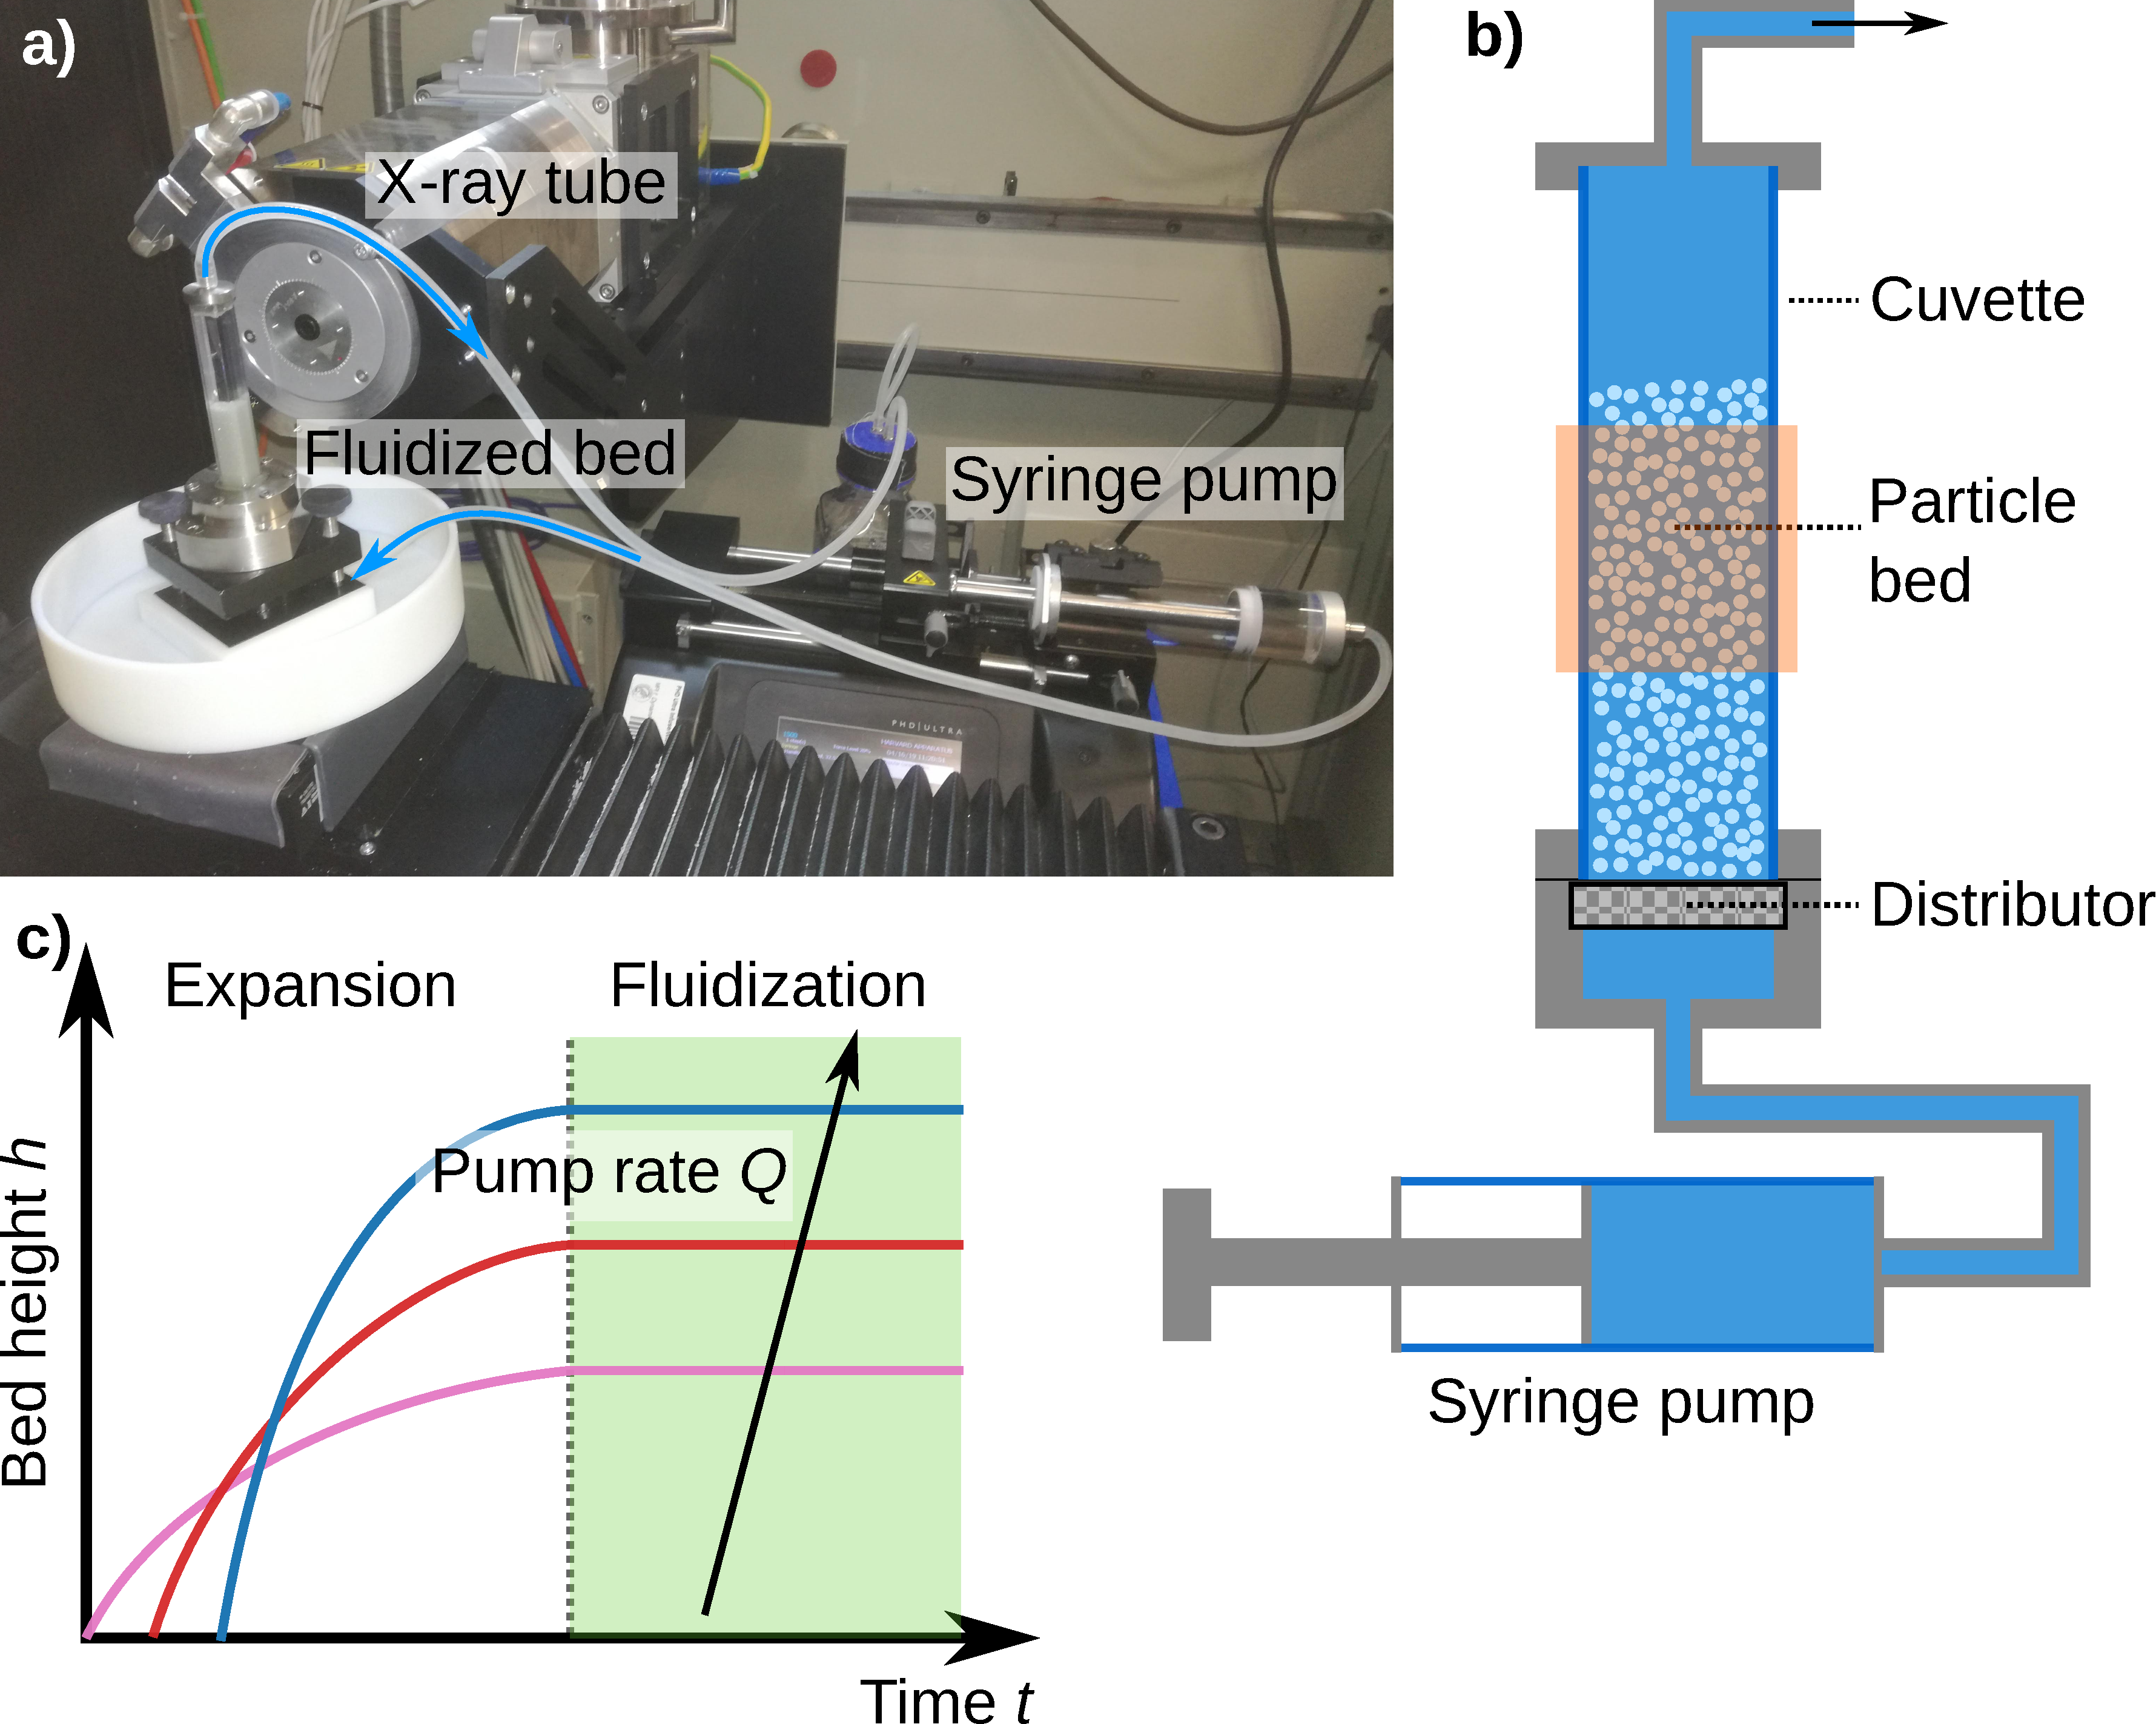
\includegraphics[width=\textwidth]{Sources/X-DFA/experiment-fluidized_bed_1.pdf}}
\end{textblock}

%\begin{textblock}{0.6}(0.4,0.9)
%	$0.45 < \Phi < 0.56$
%\end{textblock}


\begin{textblock}{0.3}(0.65,0.1)
	\centering
	\only<1>{
		Radiogram\\
		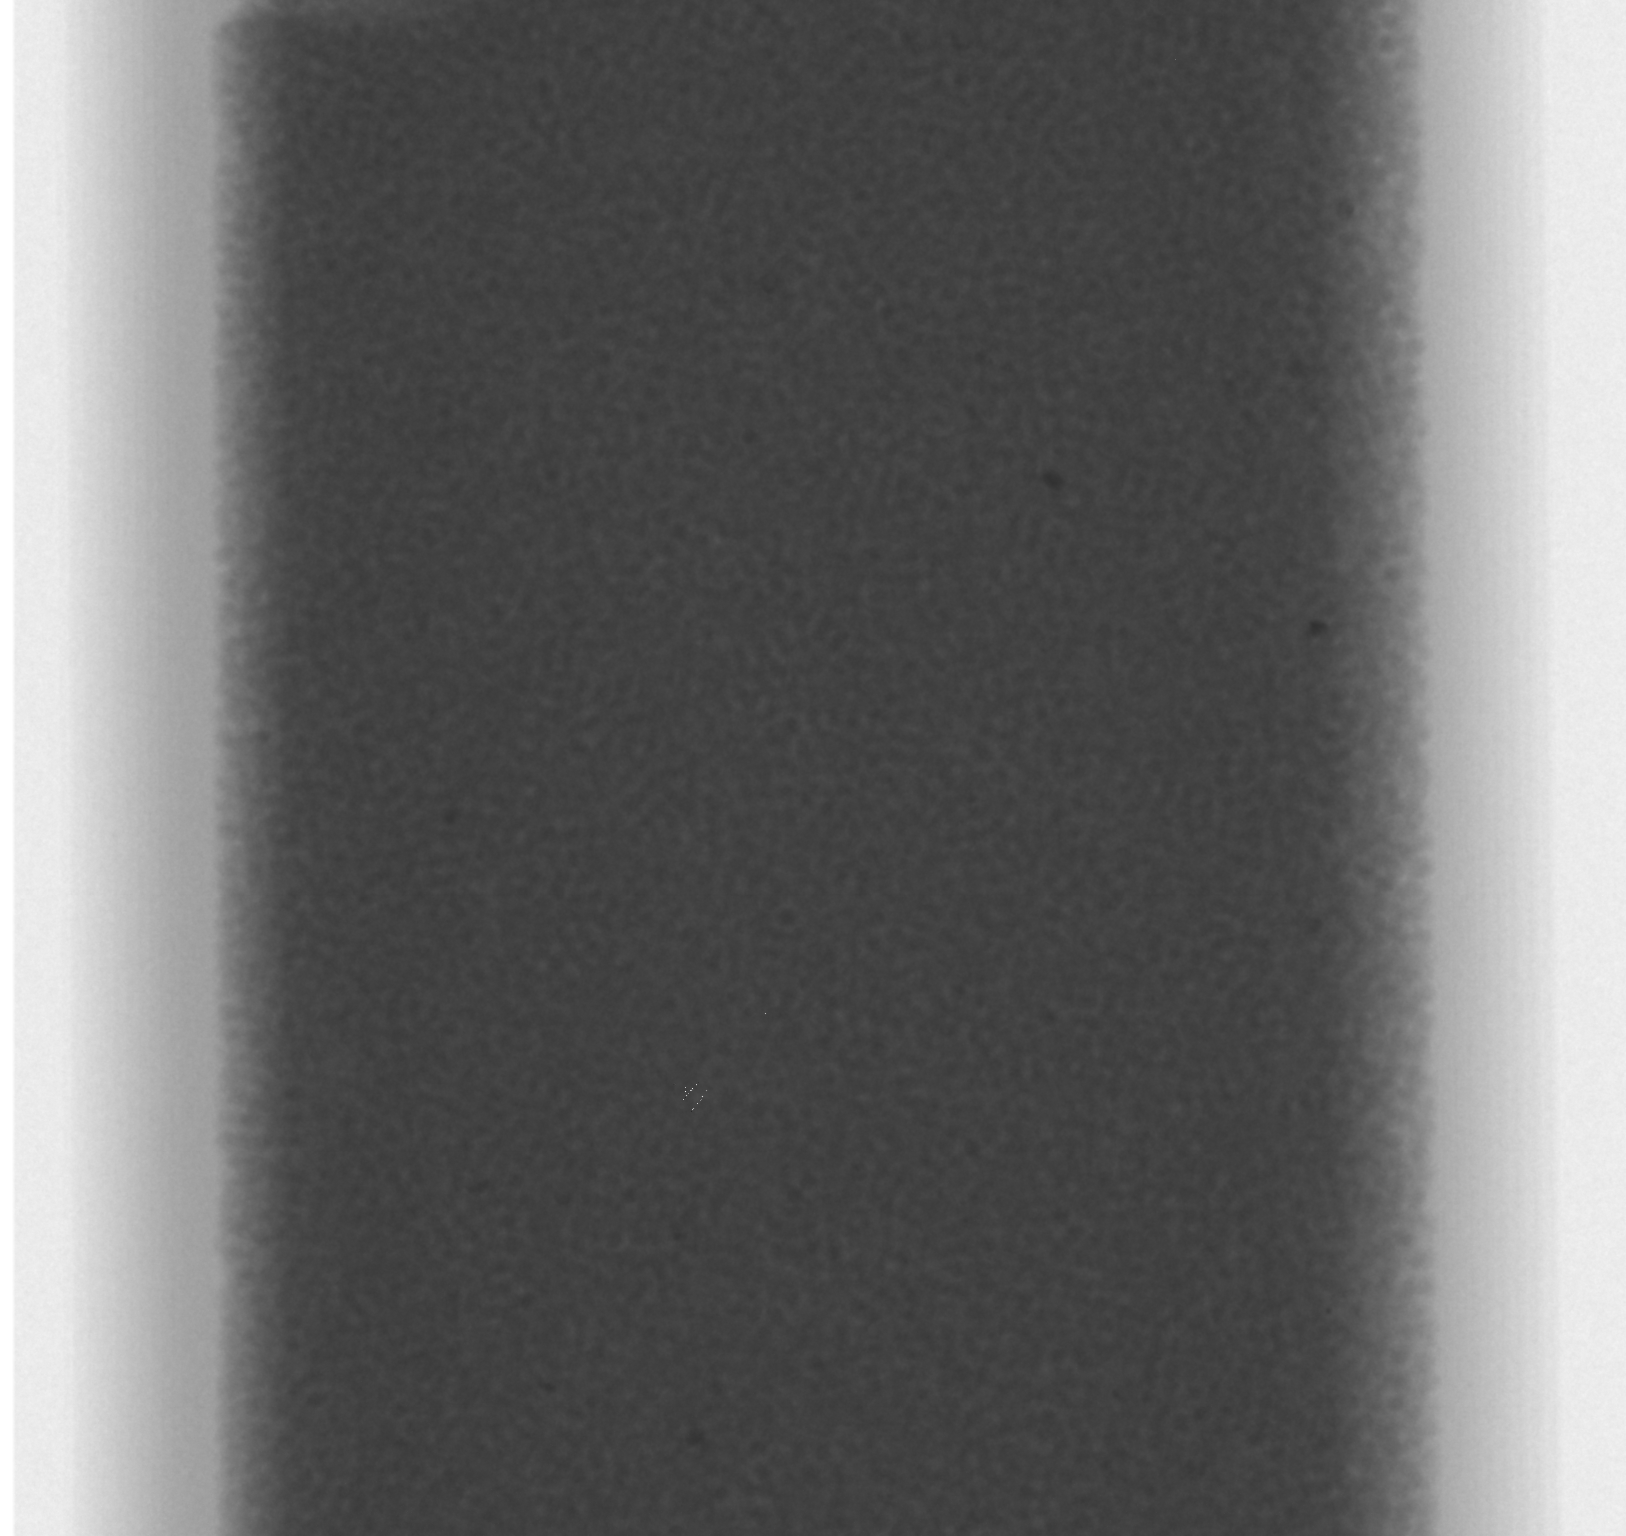
\includegraphics[width=\textwidth]{Sources/X-DFA/radiogram.png}}
\end{textblock}		

\begin{textblock}{0.3}(0.65,0.03)
	\visible<2->{
	\centering
	\textbf{Particle tracking}\\
	Contrast: $\rho_\text{tracer} > \rho_\text{bed}$}
\end{textblock}

\begin{textblock}{0.3}(0.65,0.08)
	\visible<2->{
	\vspace{0.5cm}
	\fbox{\parbox{\textwidth}{
	\movie[width = \textwidth]
	{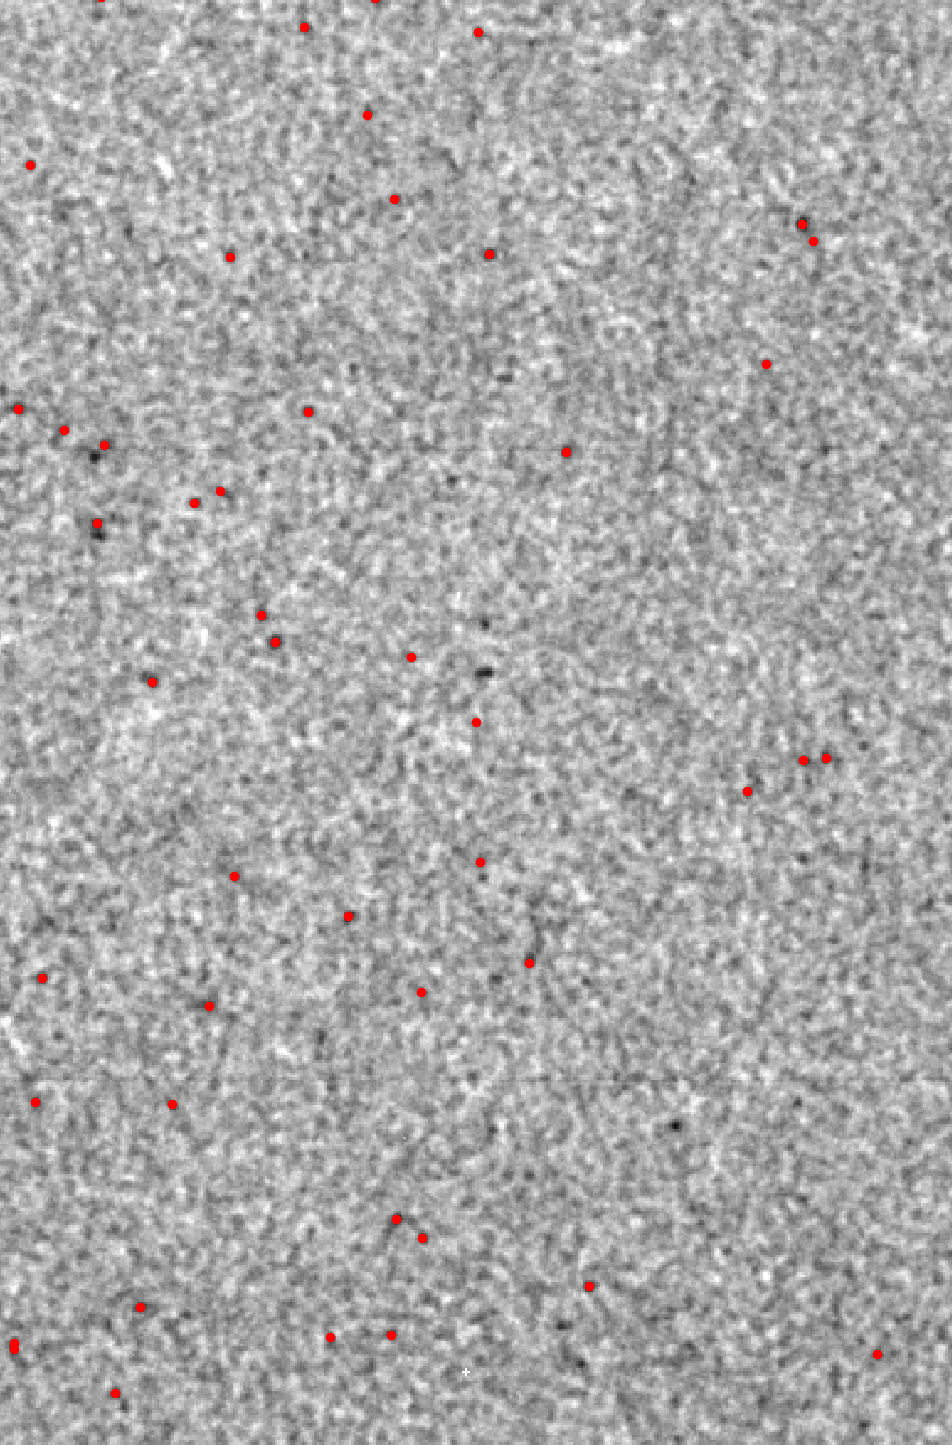
\includegraphics[width = \textwidth]{Sources/X-DFA/centroid_bronze_tracer_frame_nr_0000.png}}
	{Sources/X-DFA/centroid_bronze_tracer_4.mp4}}}}
\end{textblock}

\begin{textblock}{0.3}(0.66,0.1)
	\centering
	\visible<3->{
	\vspace{0.5cm}
	
\includegraphics[width=\textwidth]{Sources/X-DFA/cross.pdf}}
\end{textblock}
}


%% The system: A liquid fluidized bed (2)
\begin{frame}[noframenumbering]
\begin{tikzpicture}[remember picture,overlay]
\fill[blue1]
(current page.north west) rectangle ([xshift=0.5\paperwidth,yshift=0.33\paperheight]current page.west|-{pic cs:end});
\end{tikzpicture}

\begin{textblock}{0.6}(0.02,0.03)
	\textcolor{white}{
		\Large The system: A liquid fluidized bed}
\end{textblock}

\begin{textblock}{0.6}(0.03,0.12)
	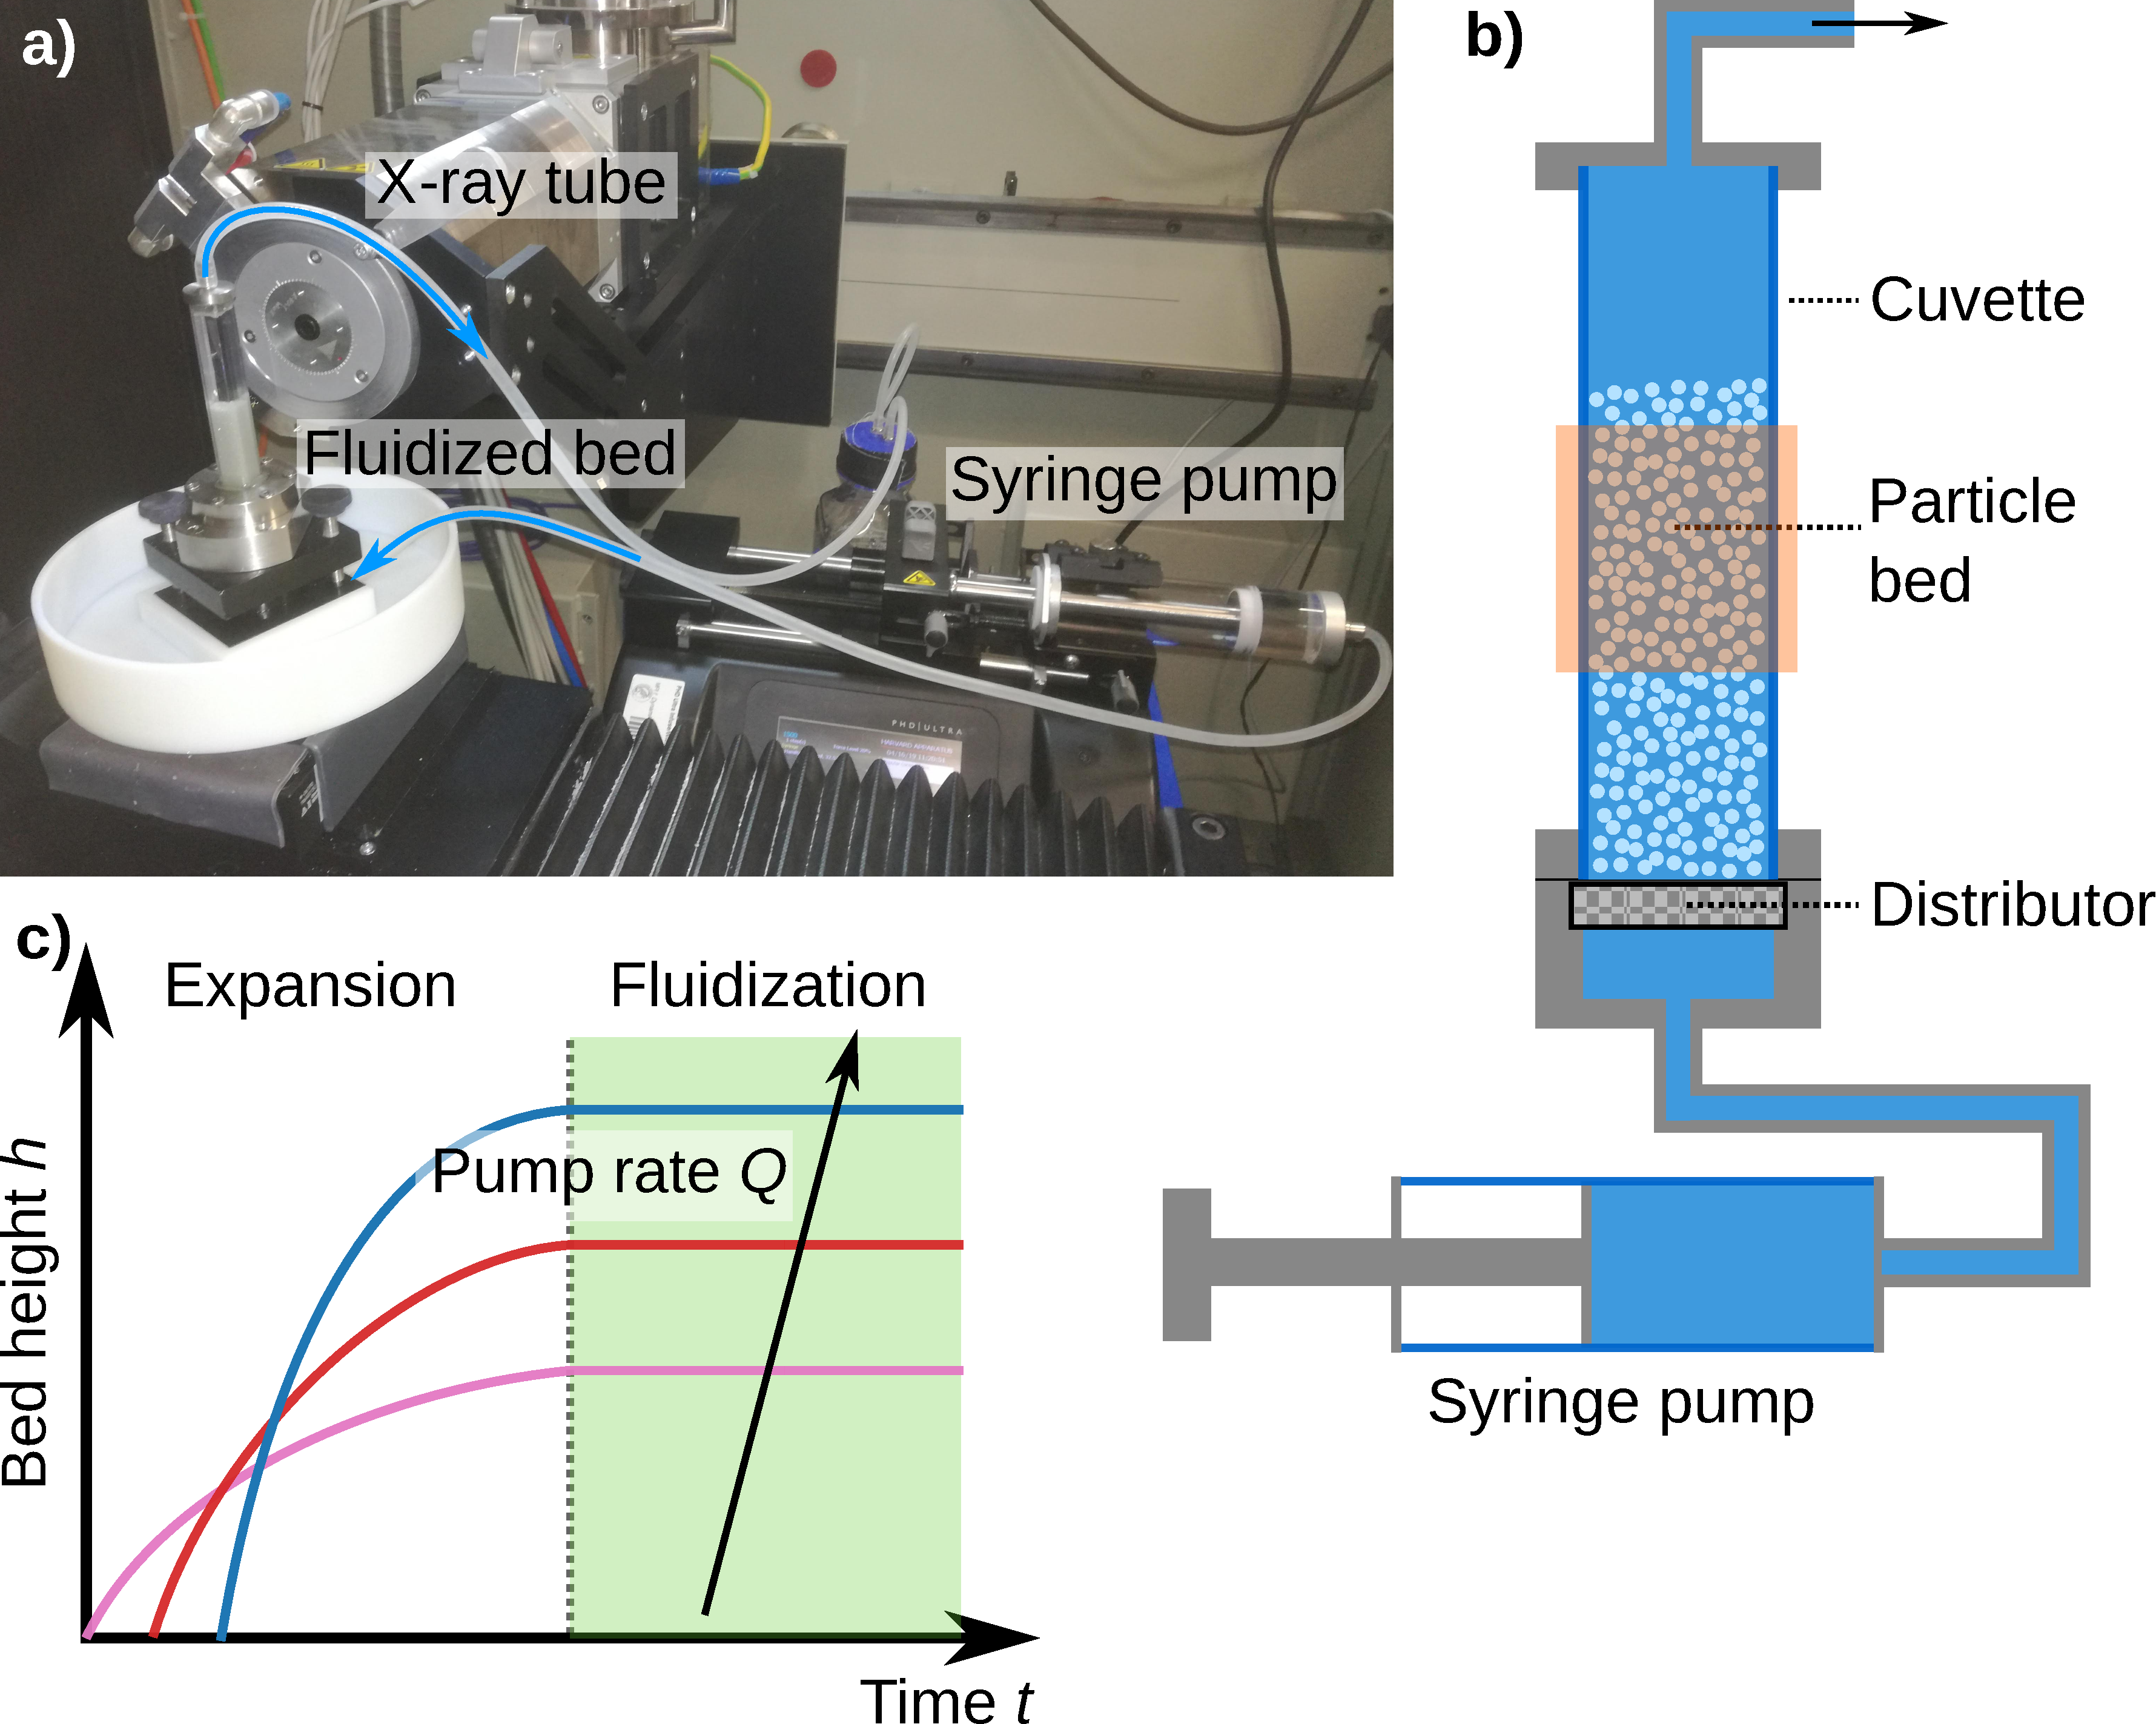
\includegraphics[width=\textwidth]{Sources/X-DFA/experiment-fluidized_bed_1.pdf}
\end{textblock}

%\begin{textblock}{0.6}(0.4,0.9)
%	$0.45 < \Phi < 0.56$
%\end{textblock}


\begin{textblock}{0.3}(0.65,0.03)
	\centering
	Radiogram\\
	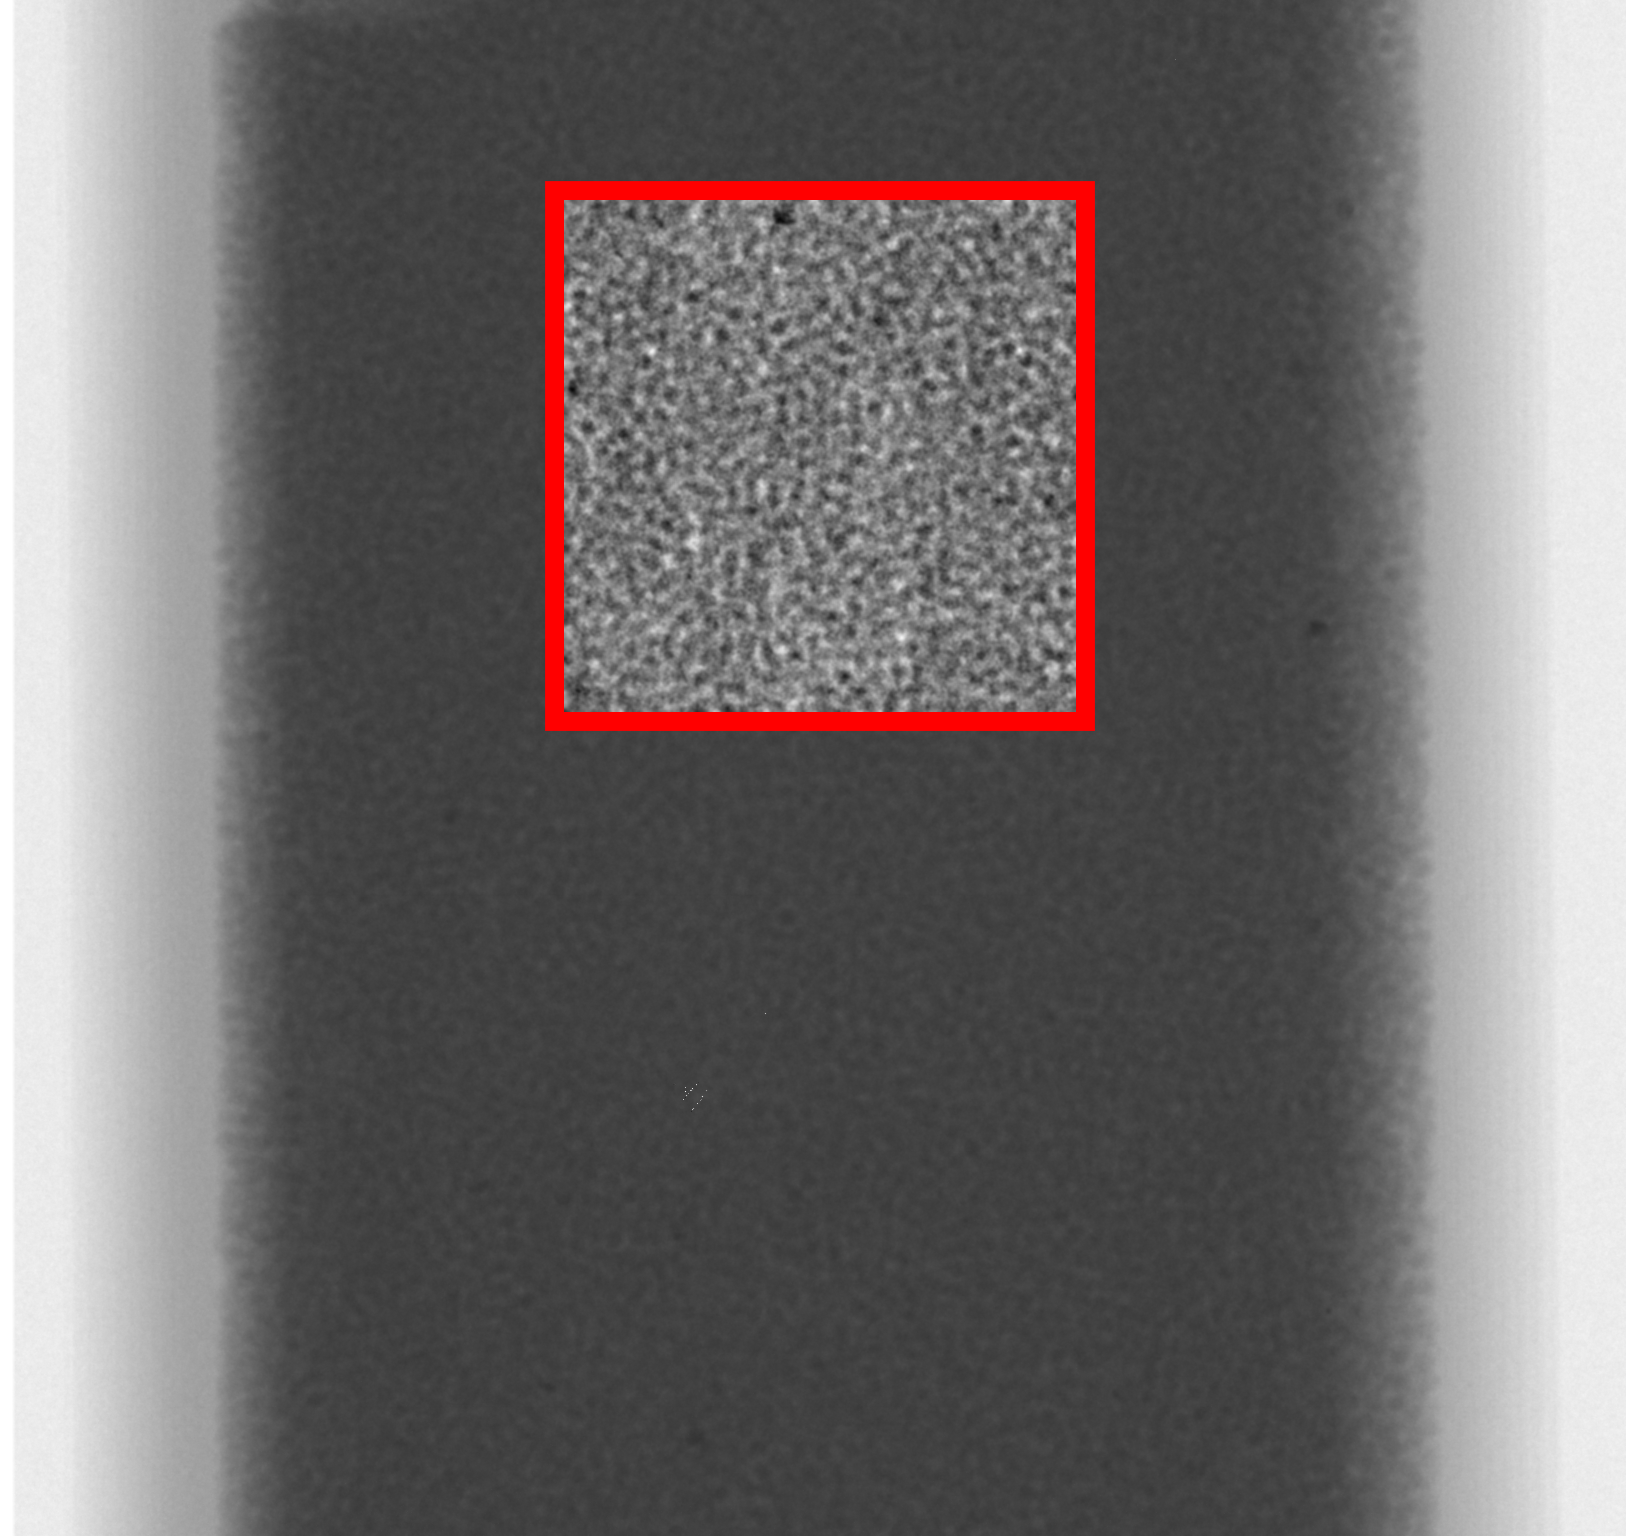
\includegraphics[width=\textwidth]{Sources/X-DFA/radiogram_ROI_marked.png}
\end{textblock}		

\begin{textblock}{0.3}(0.65,0.6)
	\centering
	\fbox{\parbox{0.64\textwidth}{
	\movie[height=0.65\textwidth, poster]
	{
\includegraphics[width=0.65\textwidth]{Sources/X-DFA/cropped_80kV_340uA_38ms_0000.png}}
	{Sources/X-DFA/3500mul_per_min_cropped_roi_512x512.avi}}
	}
\end{textblock}
\end{frame}

%%%% EXTENDING DDM to X-DFA
\frame{
	\begin{textblock}{0.9}(0.05,0.03)
		\centering
		\visible<2->{
			\Large{\textcolor{red}{
					Extending\\}}}
		\textcolor{blue1}{
			\Large{Differential Dynamic Microscopy (DDM)\\}}
		\visible<2->{
			\Large{\textcolor{red}{
					to X-ray imaging}}}
	\end{textblock}
	
	
	
	\begin{textblock}{0.9}(0.05,0.3)
		\centering
		\begin{tabular}{c|c|c}
			\toprule
			& \textbf{Up to now} & \textbf{This work}\\
			\hline
			\textbf{System} & Dispersion, gels & Fluidized bed\\
			\textbf{Particles} & Colloids $<1~\upmu\si{m}$ & 
			\only<1>{Granulates $(150-180)~\upmu\si{m}$}
			\only<2>{\textcolor{red}{Granulates $(150-180)~\upmu\si{m}$}}\\
			\textbf{Volume fraction } & $\Phi \leq 0.33$ &  $0.45 < \Phi < 0.56$\\
			\textbf{imaging} & Light microscopy & 
			\only<1>{X-ray radiography}
			\only<2>{\textcolor{red}{X-ray radiography}}\\
			\textbf{Dynamics} & 
			\multicolumn{2}{c}{Brownian motion, caging, glassy, collective motion}\\
			\bottomrule
		\end{tabular}
	\end{textblock}
	
	\begin{textblock}{0.9}(0.05,0.75)
		\centering
		\visible<2->{
			\Large{\textcolor{red}{
					Digital Fourier Analysis of X-Ray radiograms (X-DFA)}}}
	\end{textblock}
	
	\begin{textblock}{0.7}(0.02,0.95)
		{\footnotesize Giavazzi \textit{et al}, PRE \textbf{80}, 031403 (2009)}
	\end{textblock}
}



%%%%%%%%%% Introduction to DDM
\frame{
\begin{tikzpicture}[remember picture,overlay]
\fill[blue1]
(current page.north west) rectangle ([xshift=12.cm,yshift=-10.cm]current page.east|-{pic cs:end});
\end{tikzpicture}
\begin{textblock}{0.9}(0.05,0.05)
	\centering
	\textcolor{white}{\huge Introduction to \\[0.1cm]
	Differential Dynamic Microscopy (DDM)}
\end{textblock}
	
\begin{textblock}{0.4}(0.05,0.25)
	\centering
		\textcolor{white}{Synthetic radiograms}\\[0.2cm]
	\movie[height = 0.6\textheight, poster, loop]
	{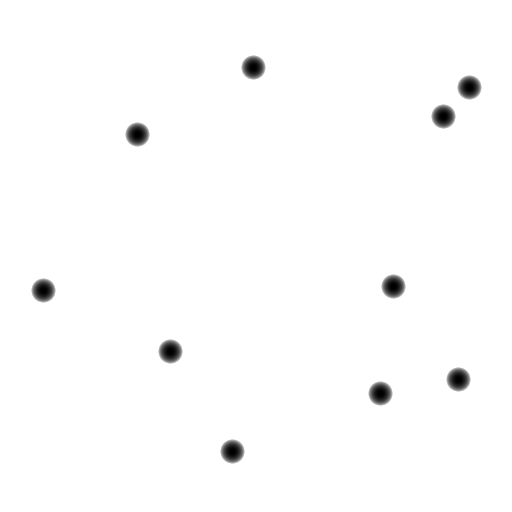
\includegraphics[height = 0.6\textheight]{Sources/X-DFA/10_particles_fake_img.png}}
	{Sources/X-DFA/10_part_1900-2100.avi}
\end{textblock}


\begin{textblock}{0.45}(0.55,0.25)
\centering
	\textcolor{white}{Particle trajectory}\\[0.2cm]
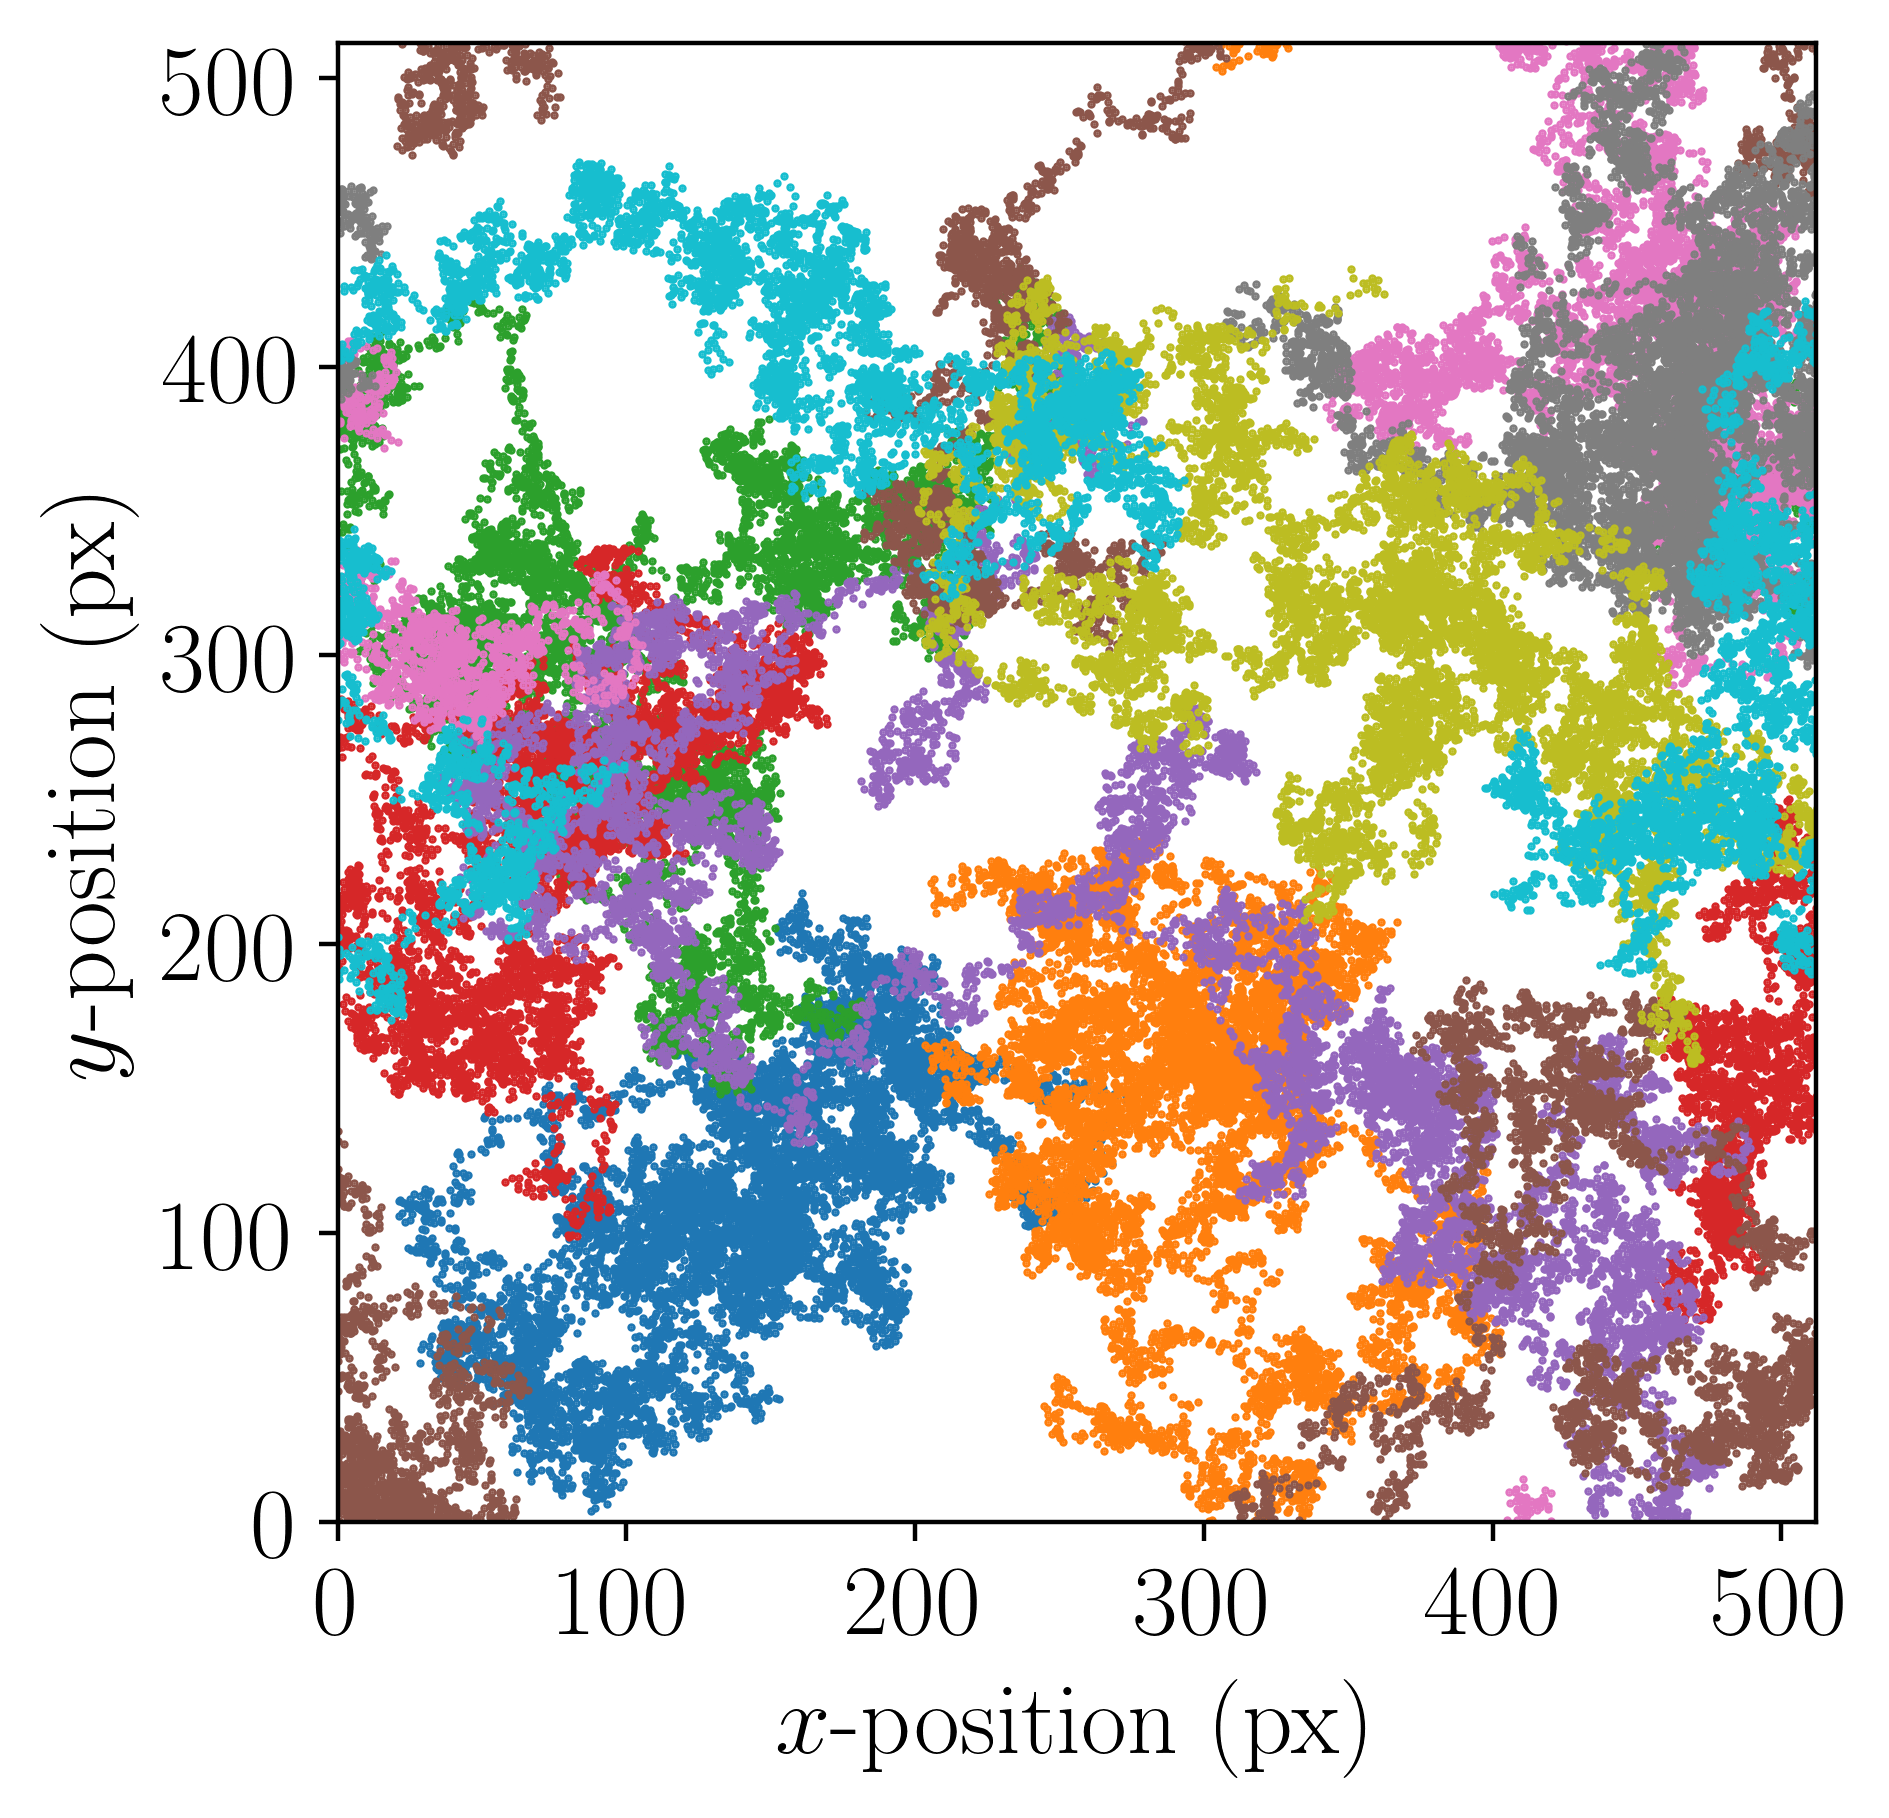
\includegraphics[height = 0.6\textheight]{Sources/X-DFA/trajectory_plot_nPart10.png}
\end{textblock}
}








\frame{
\begin{tikzpicture}[remember picture,overlay]
\fill[blue1]
(current page.north west) rectangle ([xshift=0.52\paperwidth,yshift=0.33\paperheight]current page.west|-{pic cs:end});
\end{tikzpicture}
	
\begin{textblock}{0.6}(0.02,0.03)
	\textcolor{white}{
		\Large The image structure function $D(\mathbf{q}, \tau)$}
\end{textblock}

\begin{textblock}{0.7}(0.15,0.11)
	\only<1>{
	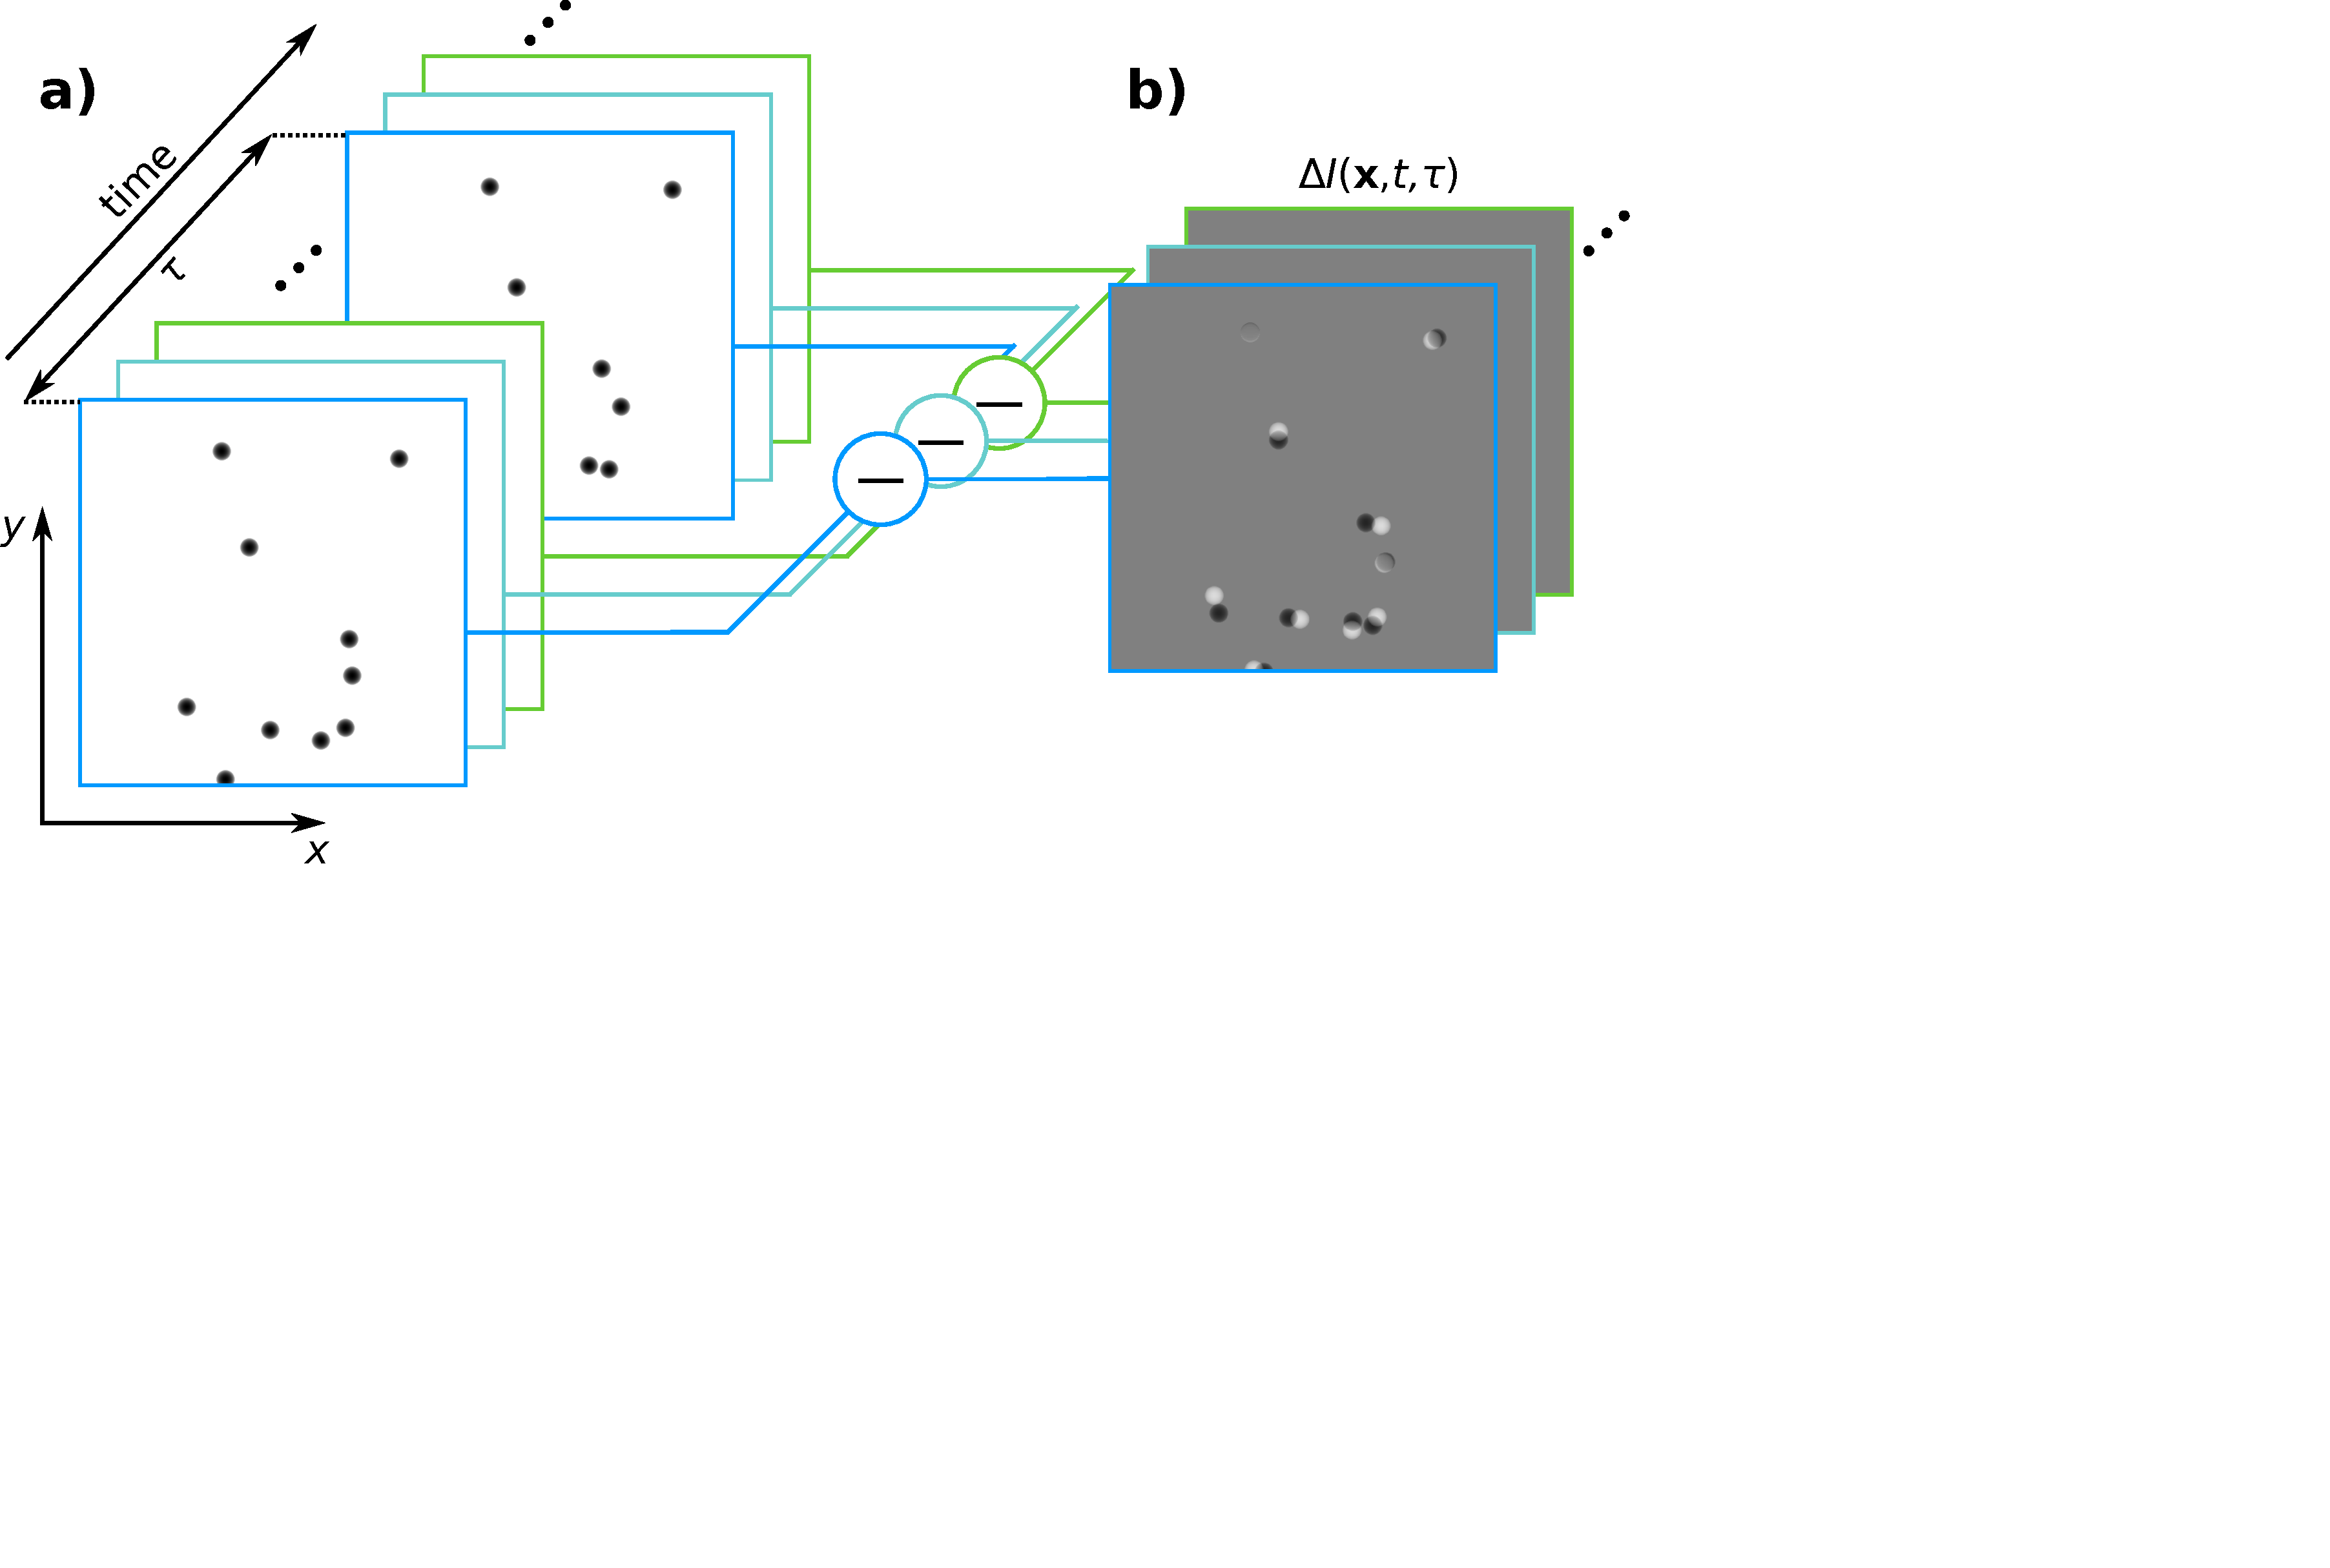
\includegraphics[width=\textwidth]{Sources/X-DFA/image_structure_function_ab.pdf}}
	\only<2>{
	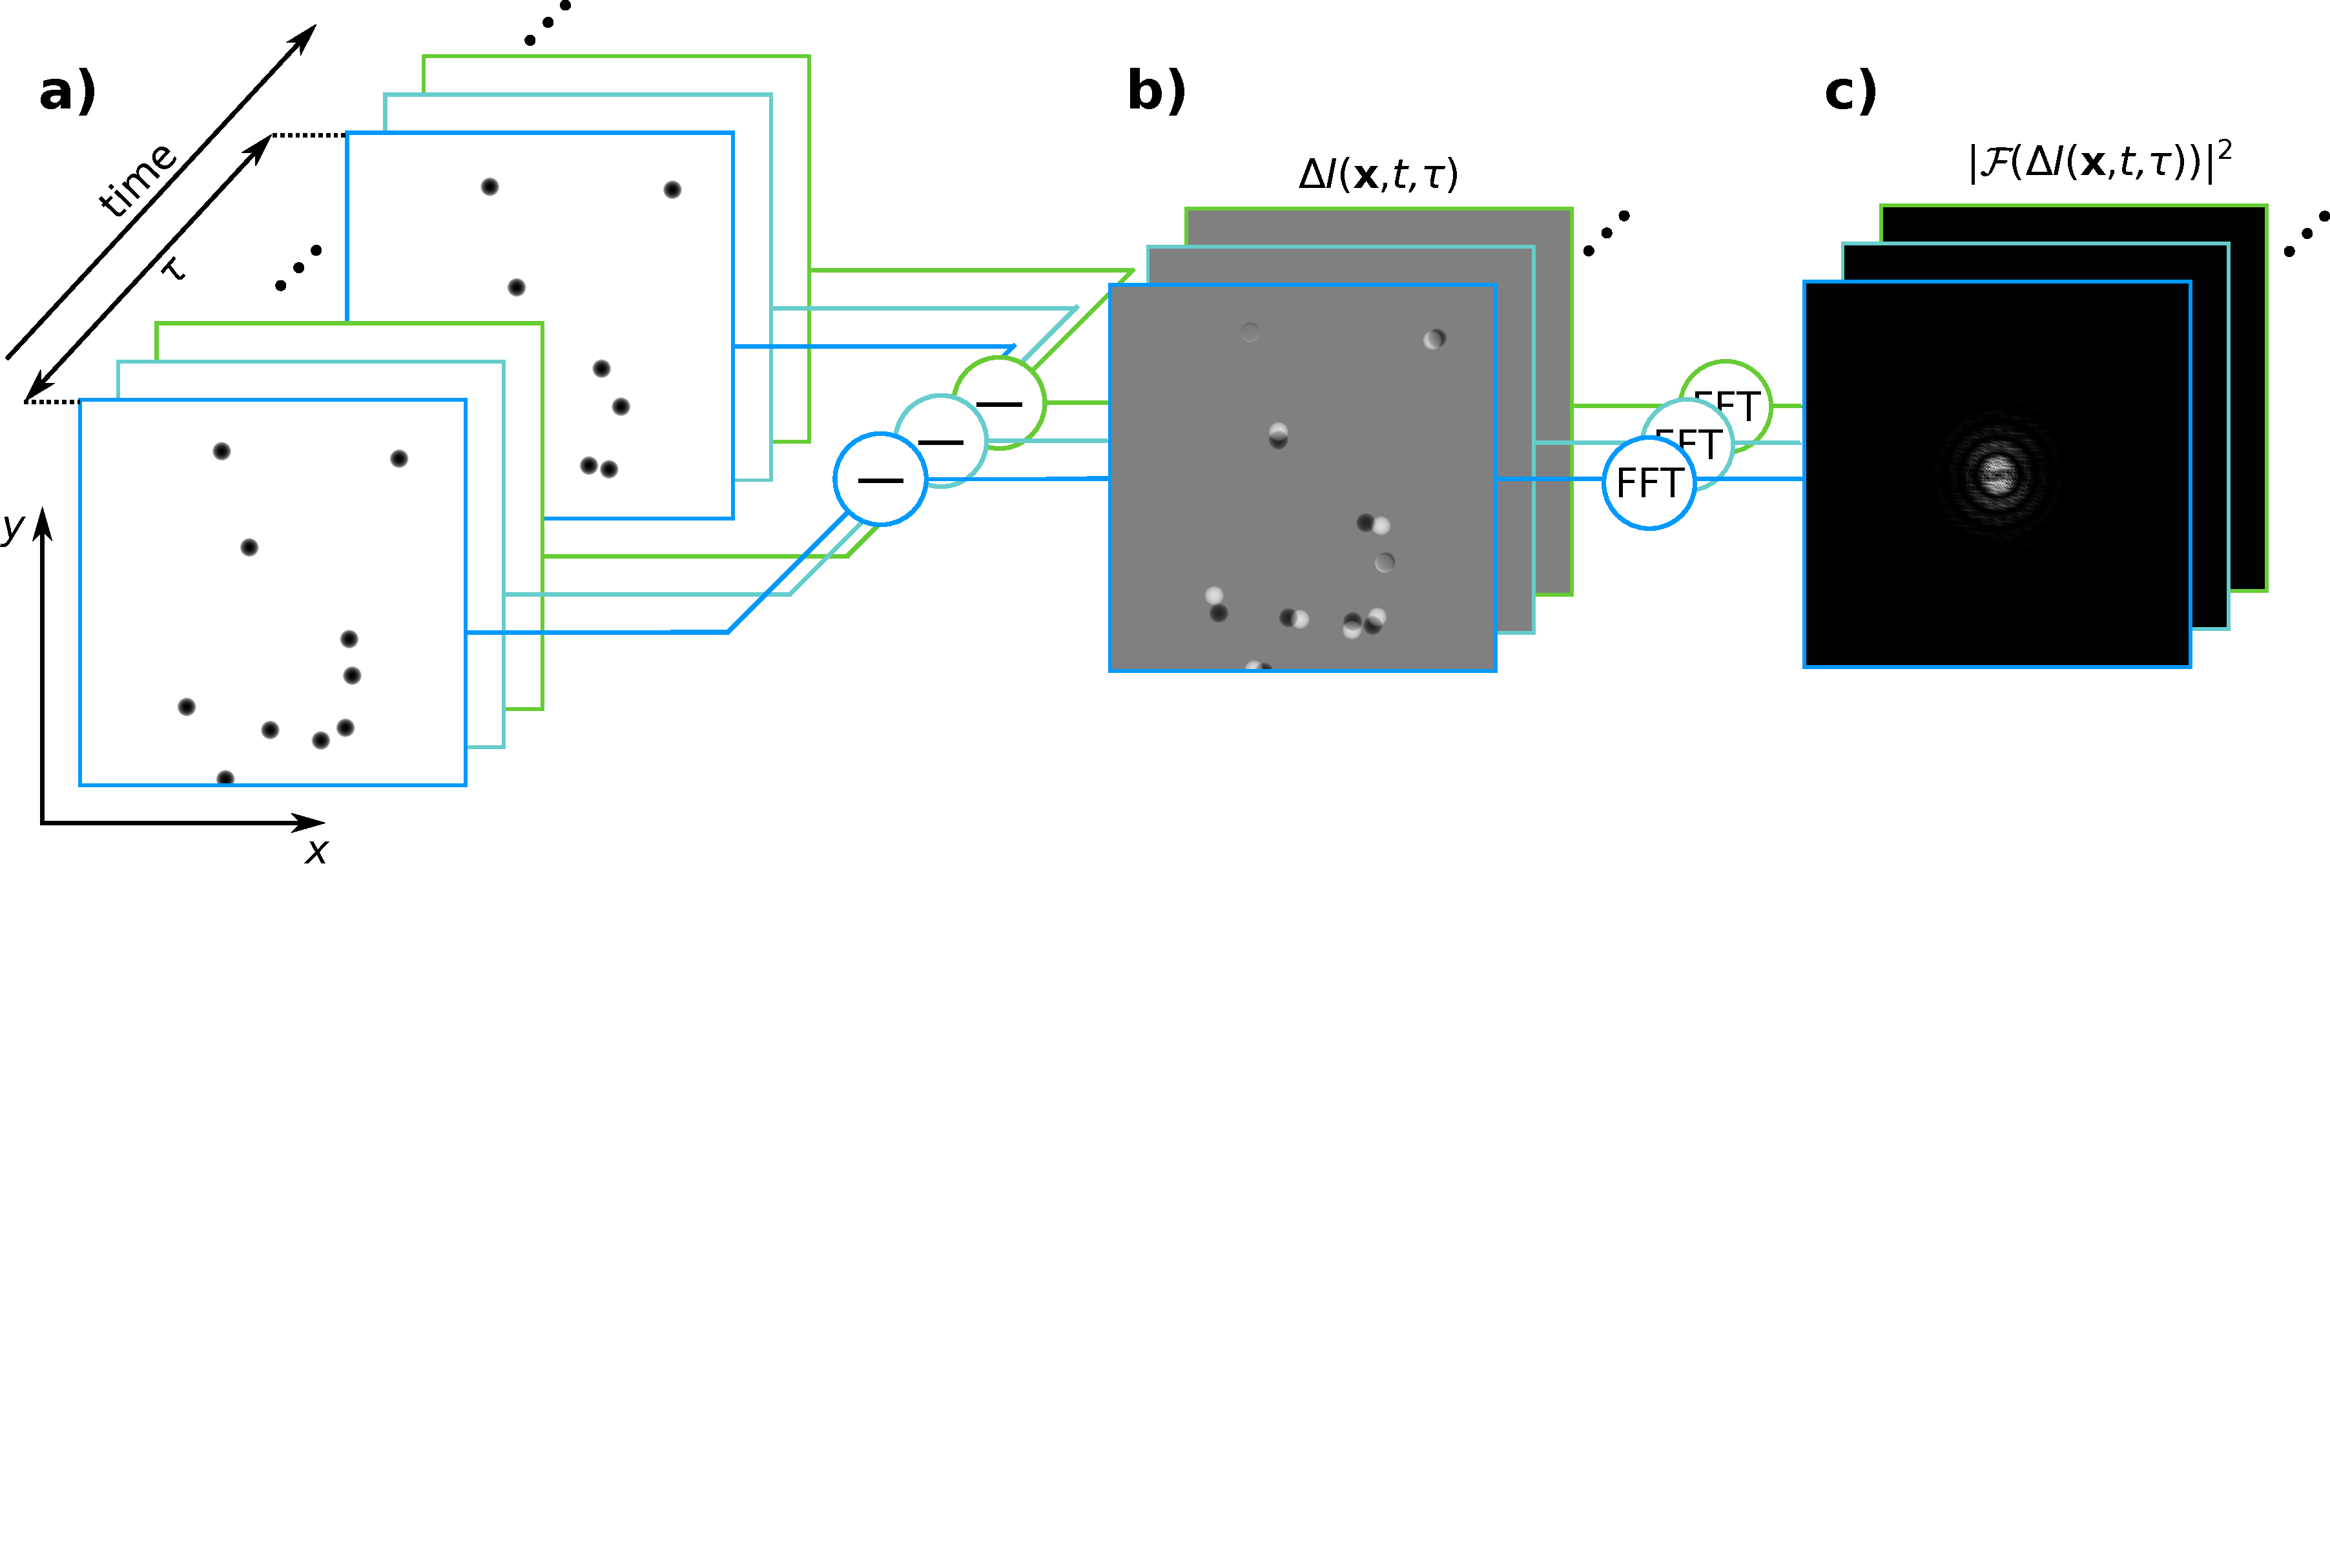
\includegraphics[width=\textwidth]{Sources/X-DFA/image_structure_function_abc.pdf}}
	\only<3>{
	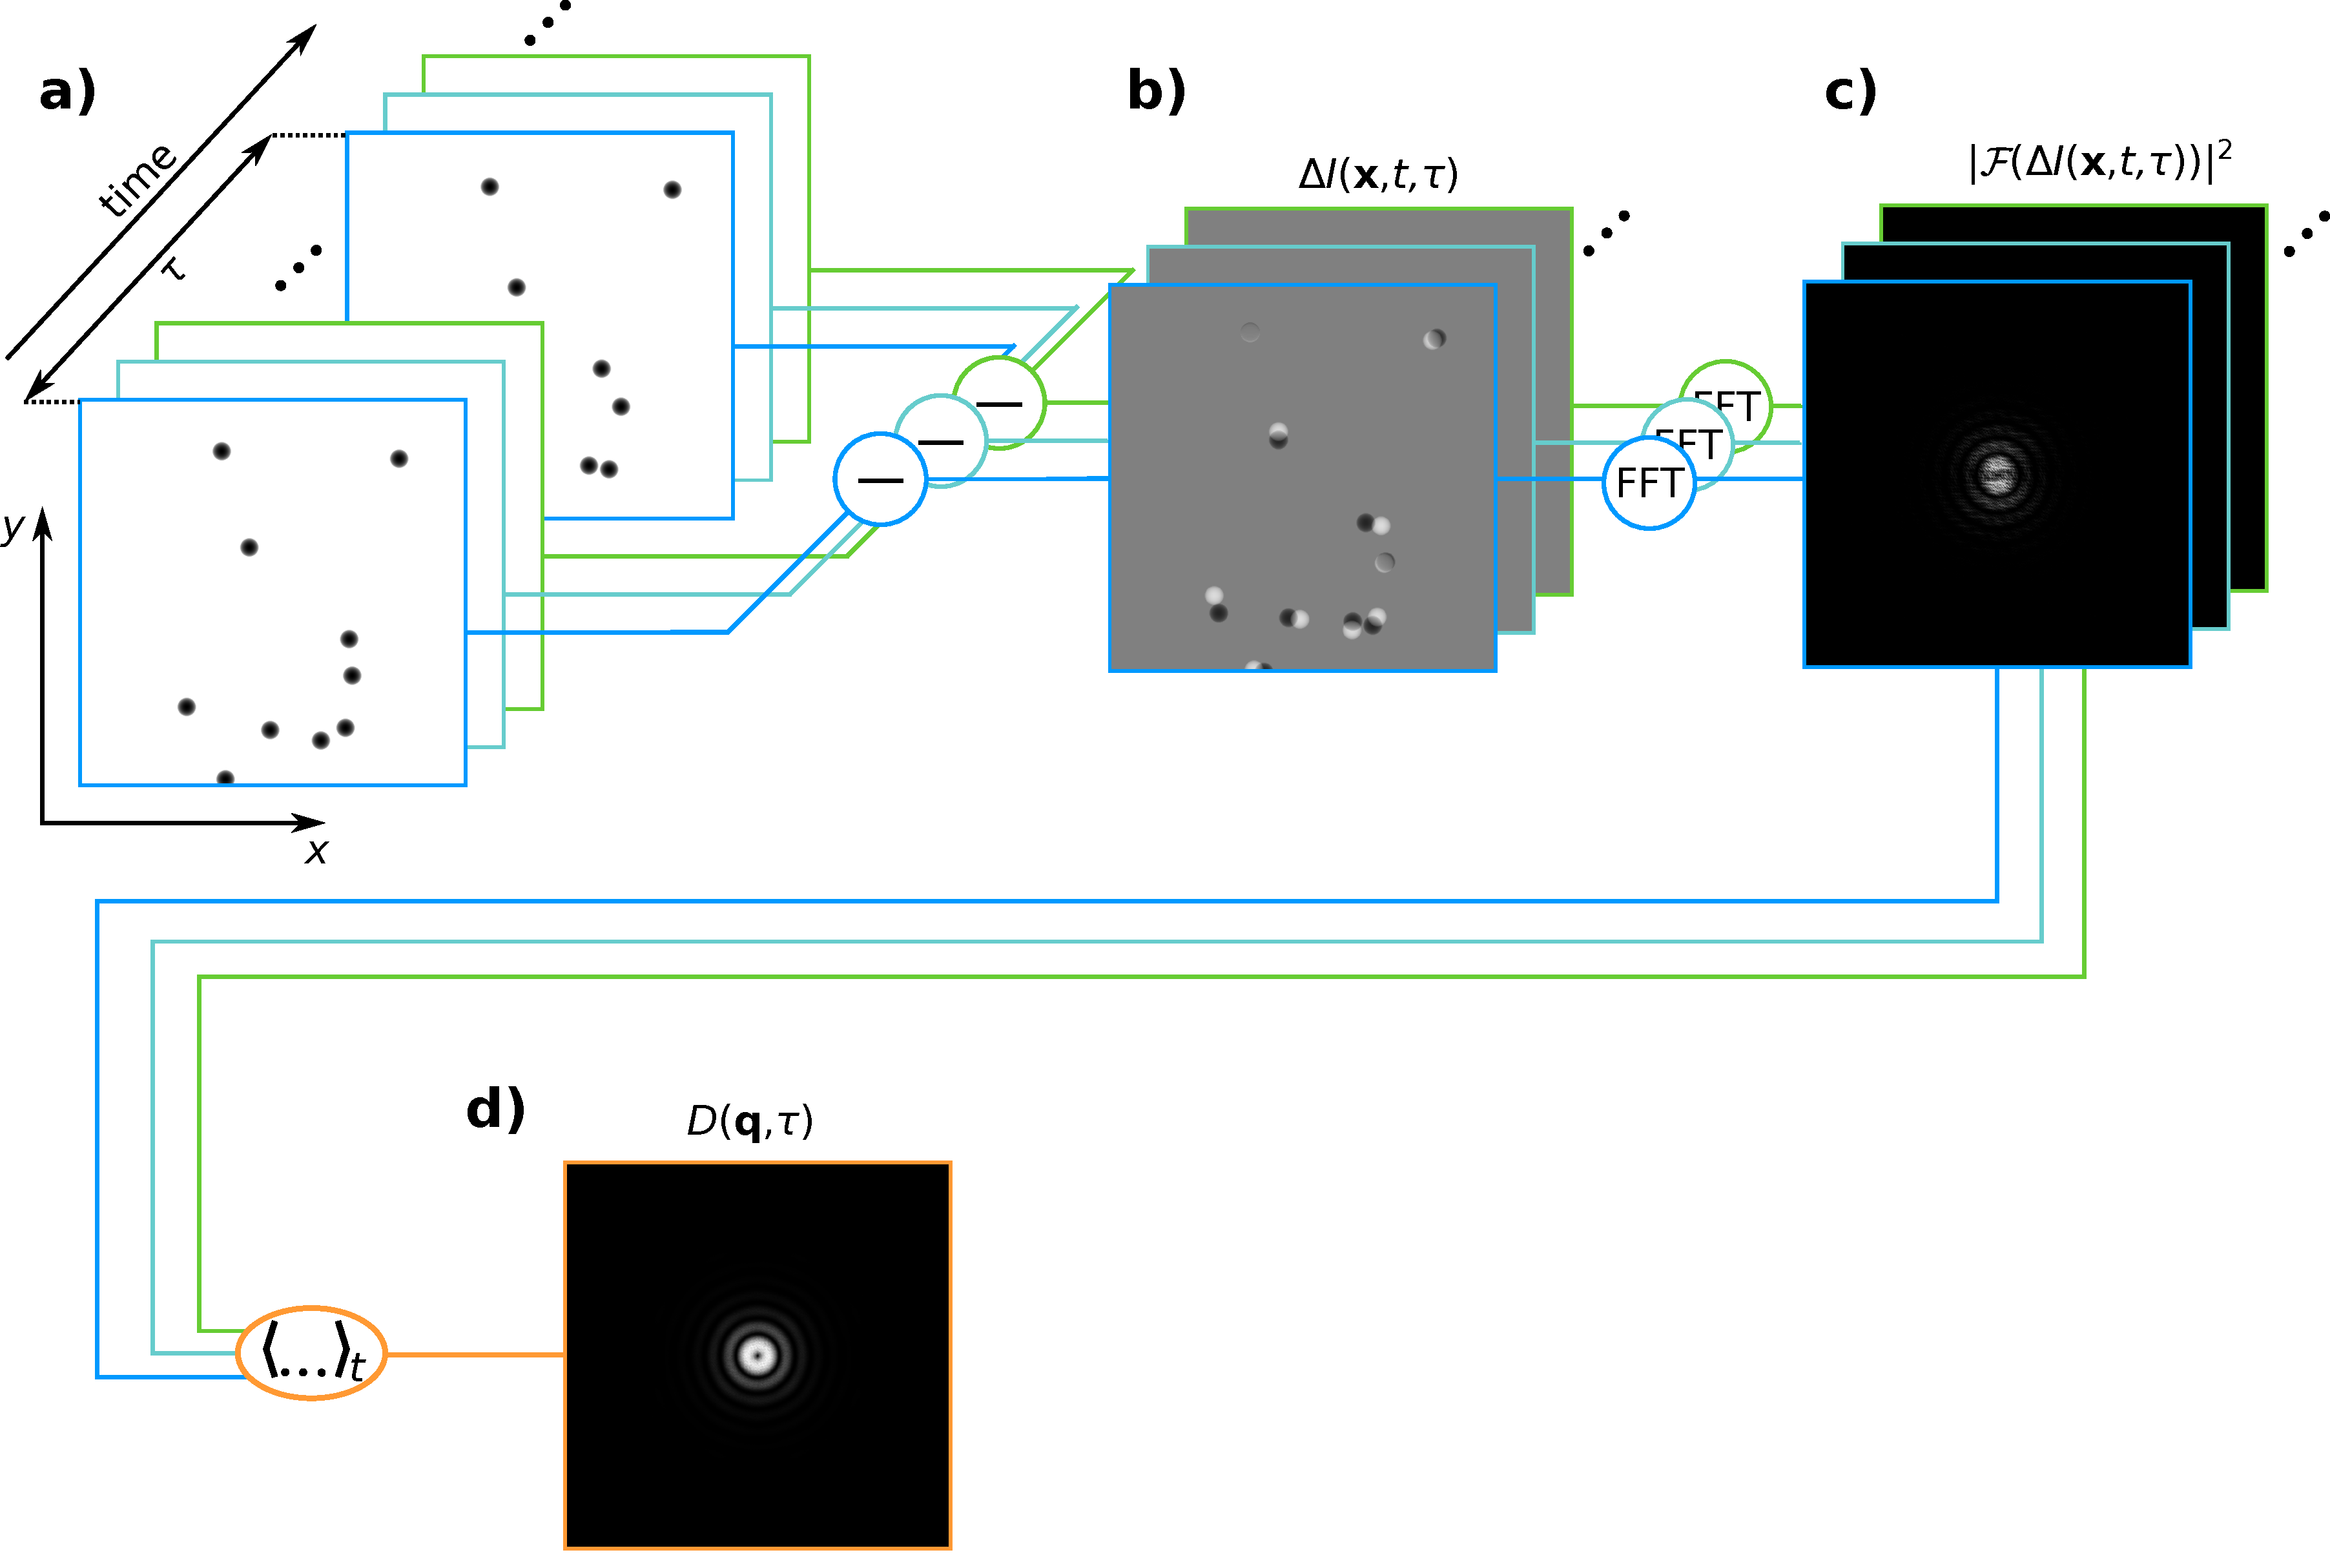
\includegraphics[width=\textwidth]{Sources/X-DFA/image_structure_function_abcd.pdf}}
	\only<4>{
	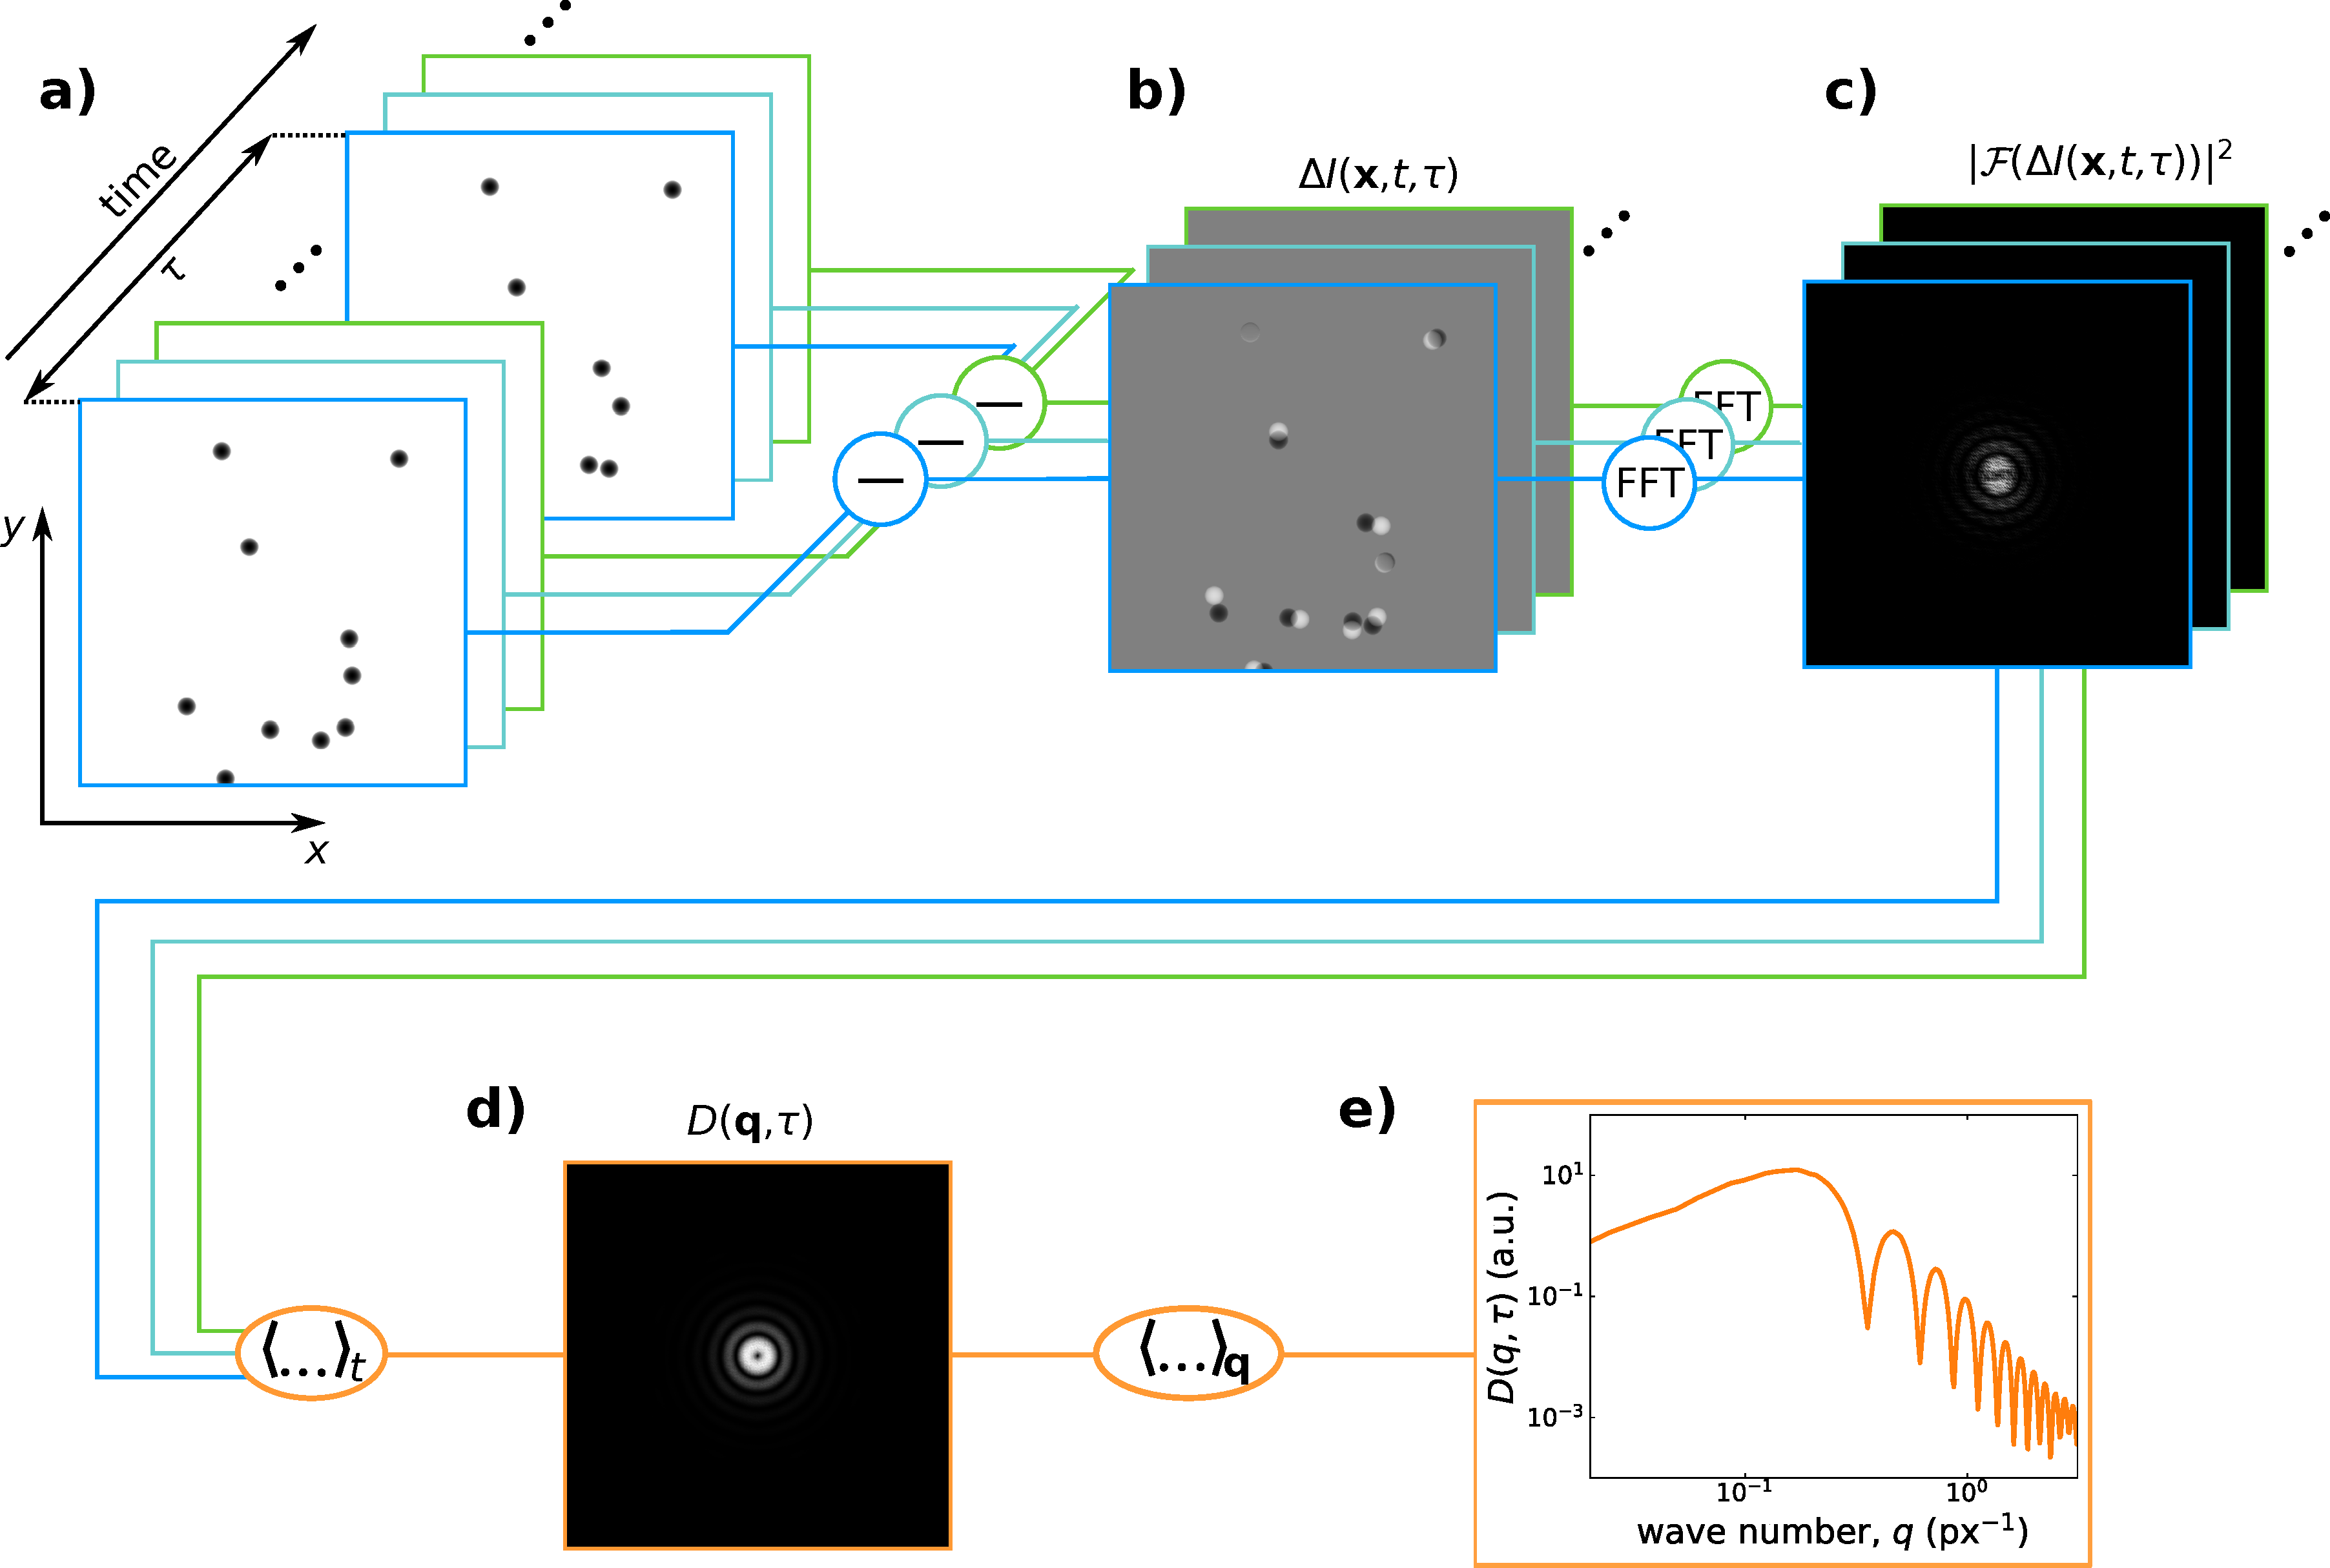
\includegraphics[width=\textwidth]{Sources/X-DFA/image_structure_function.pdf}}
\end{textblock}

\begin{textblock}{0.7}(0.02,0.95)
	\scriptsize{Giavazzi \textit{et al}, PRE \textbf{80}, 031403 (2009)}
\end{textblock}
}



%%%%%%%%%%%%%%%%%%%%%%%%%%%%%%%%%%%%%%%%%%%%%%%%%%%%%%%%%%%%%%%%%%%%%%%%%%%%%%%%%%%%%%%%%%%%%%%
%%%%%%% Build the image structure function for every time step
\frame{
\begin{tikzpicture}[remember picture,overlay]
\fill[blue1]
(current page.north west) rectangle ([xshift=0.52\paperwidth,yshift=0.33\paperheight]current page.west|-{pic cs:end});
\end{tikzpicture}

\begin{textblock}{0.6}(0.02,0.03)
	\textcolor{white}{
		\Large The image structure function $D(q, \tau)$}
\end{textblock}

	\begin{textblock}{0.3}(0.05,0.1)
	\only<1>{
	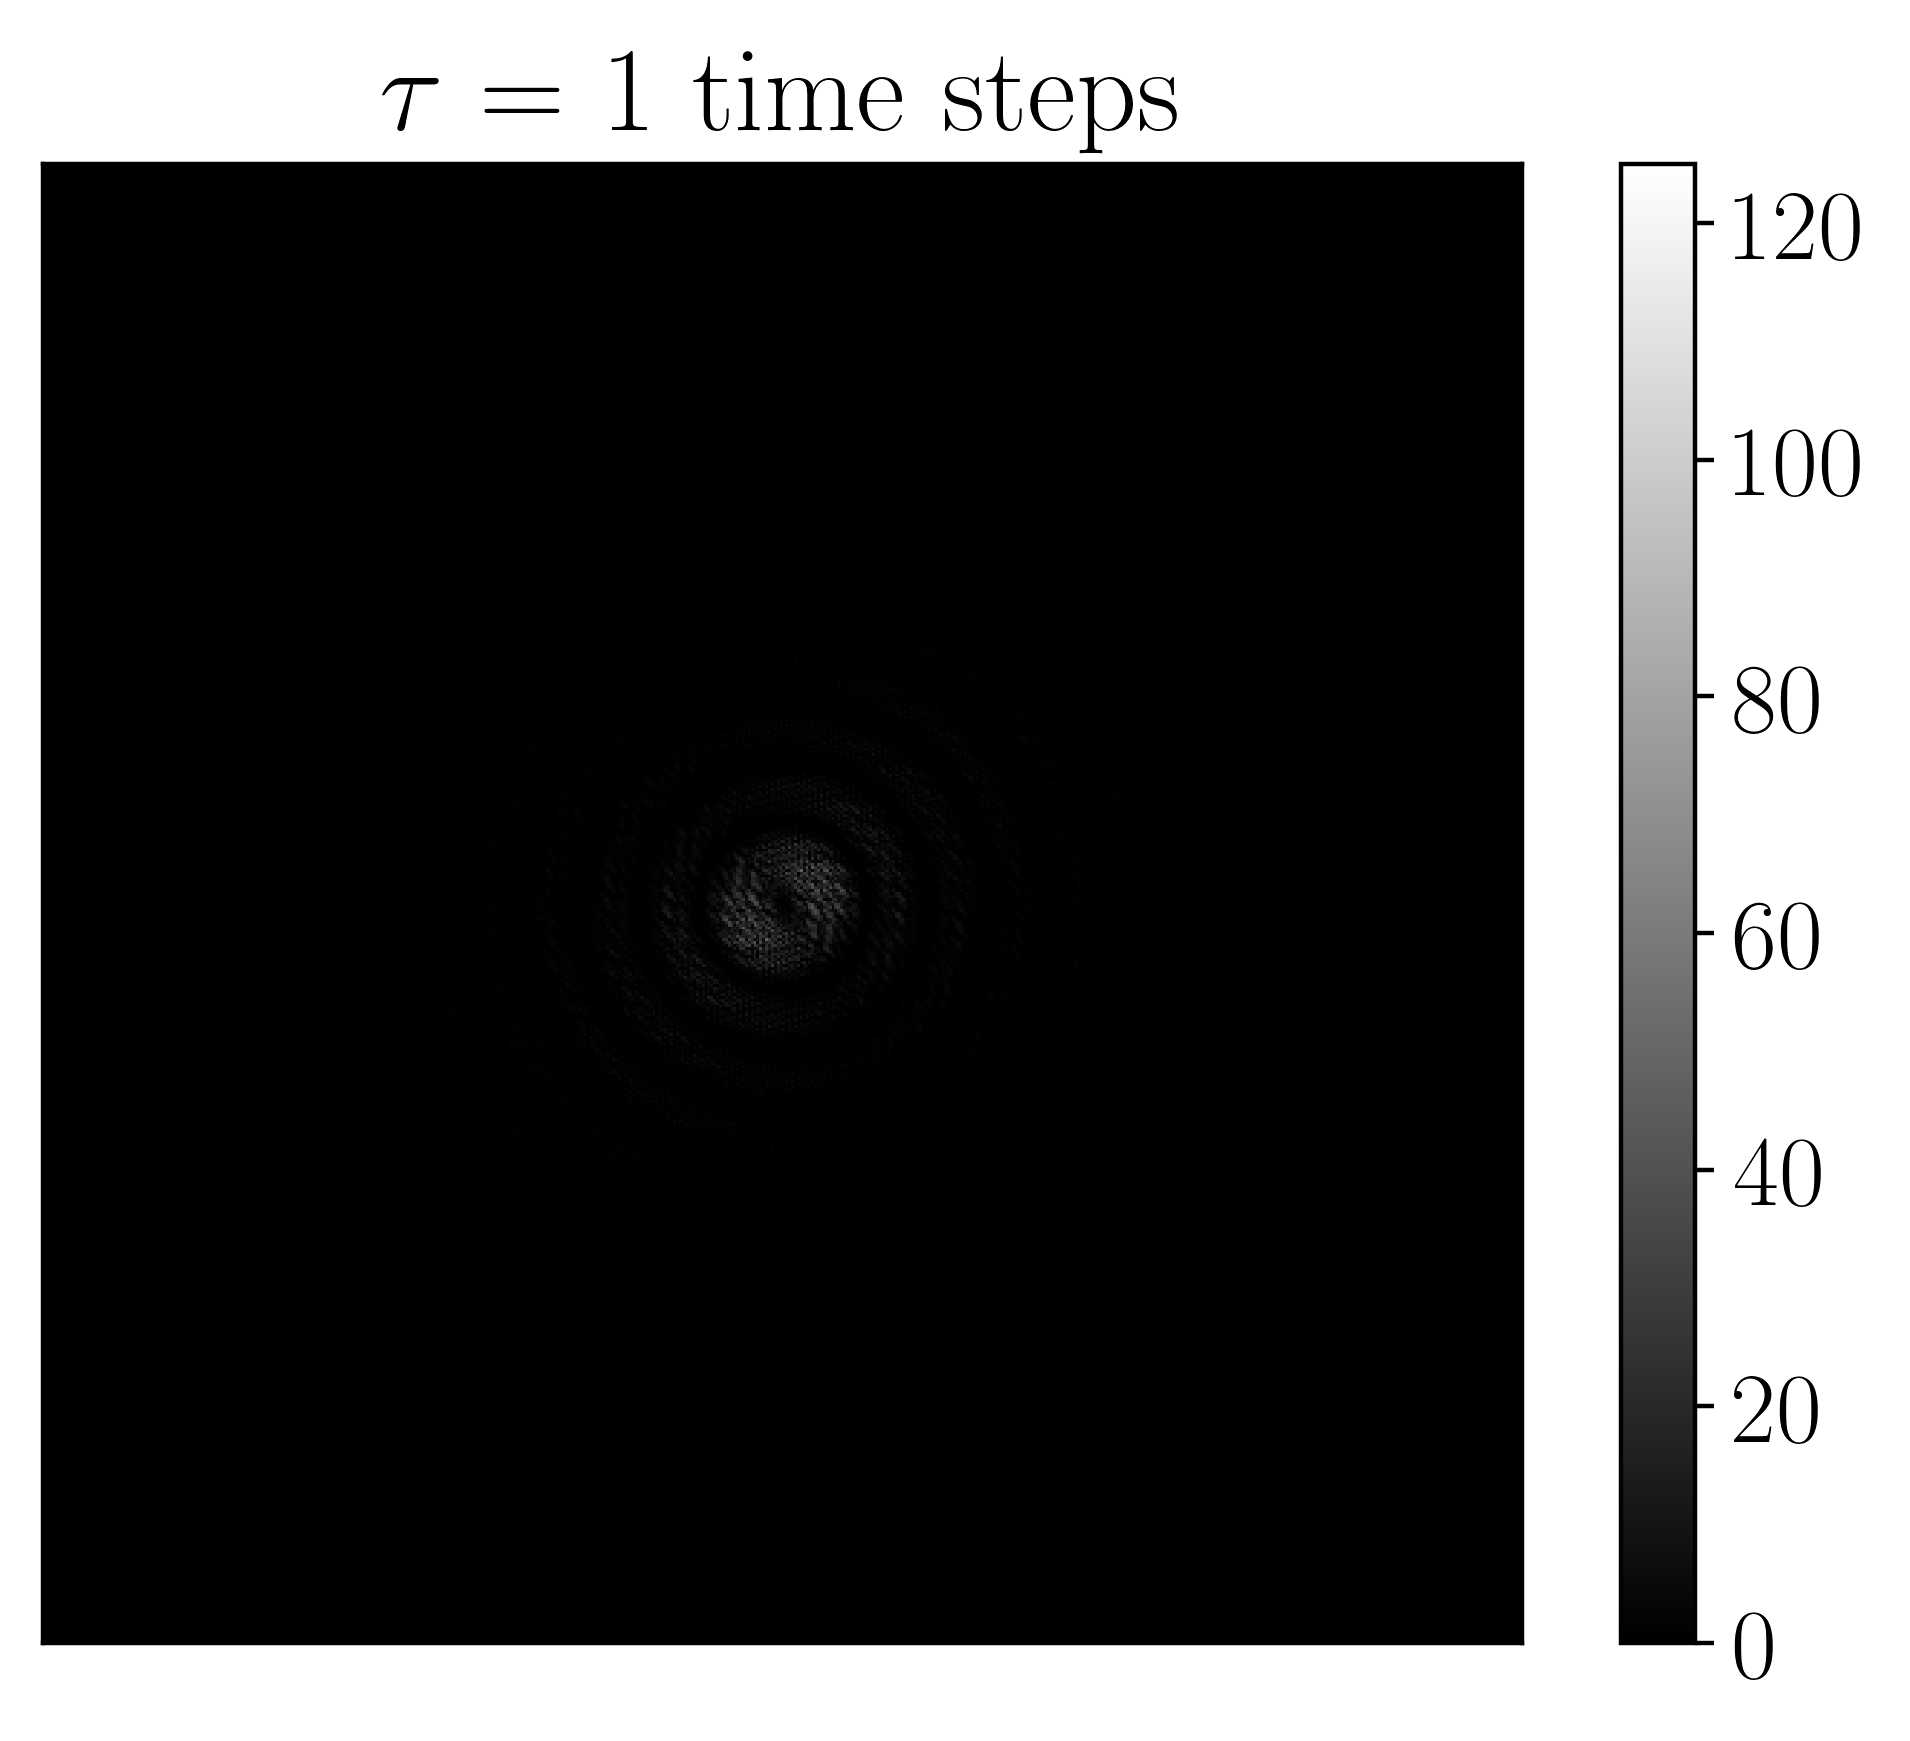
\includegraphics[width=\textwidth]
	{Sources/X-DFA/Mag_Spectrum_d_img_00000.png}}

	\only<2>{
	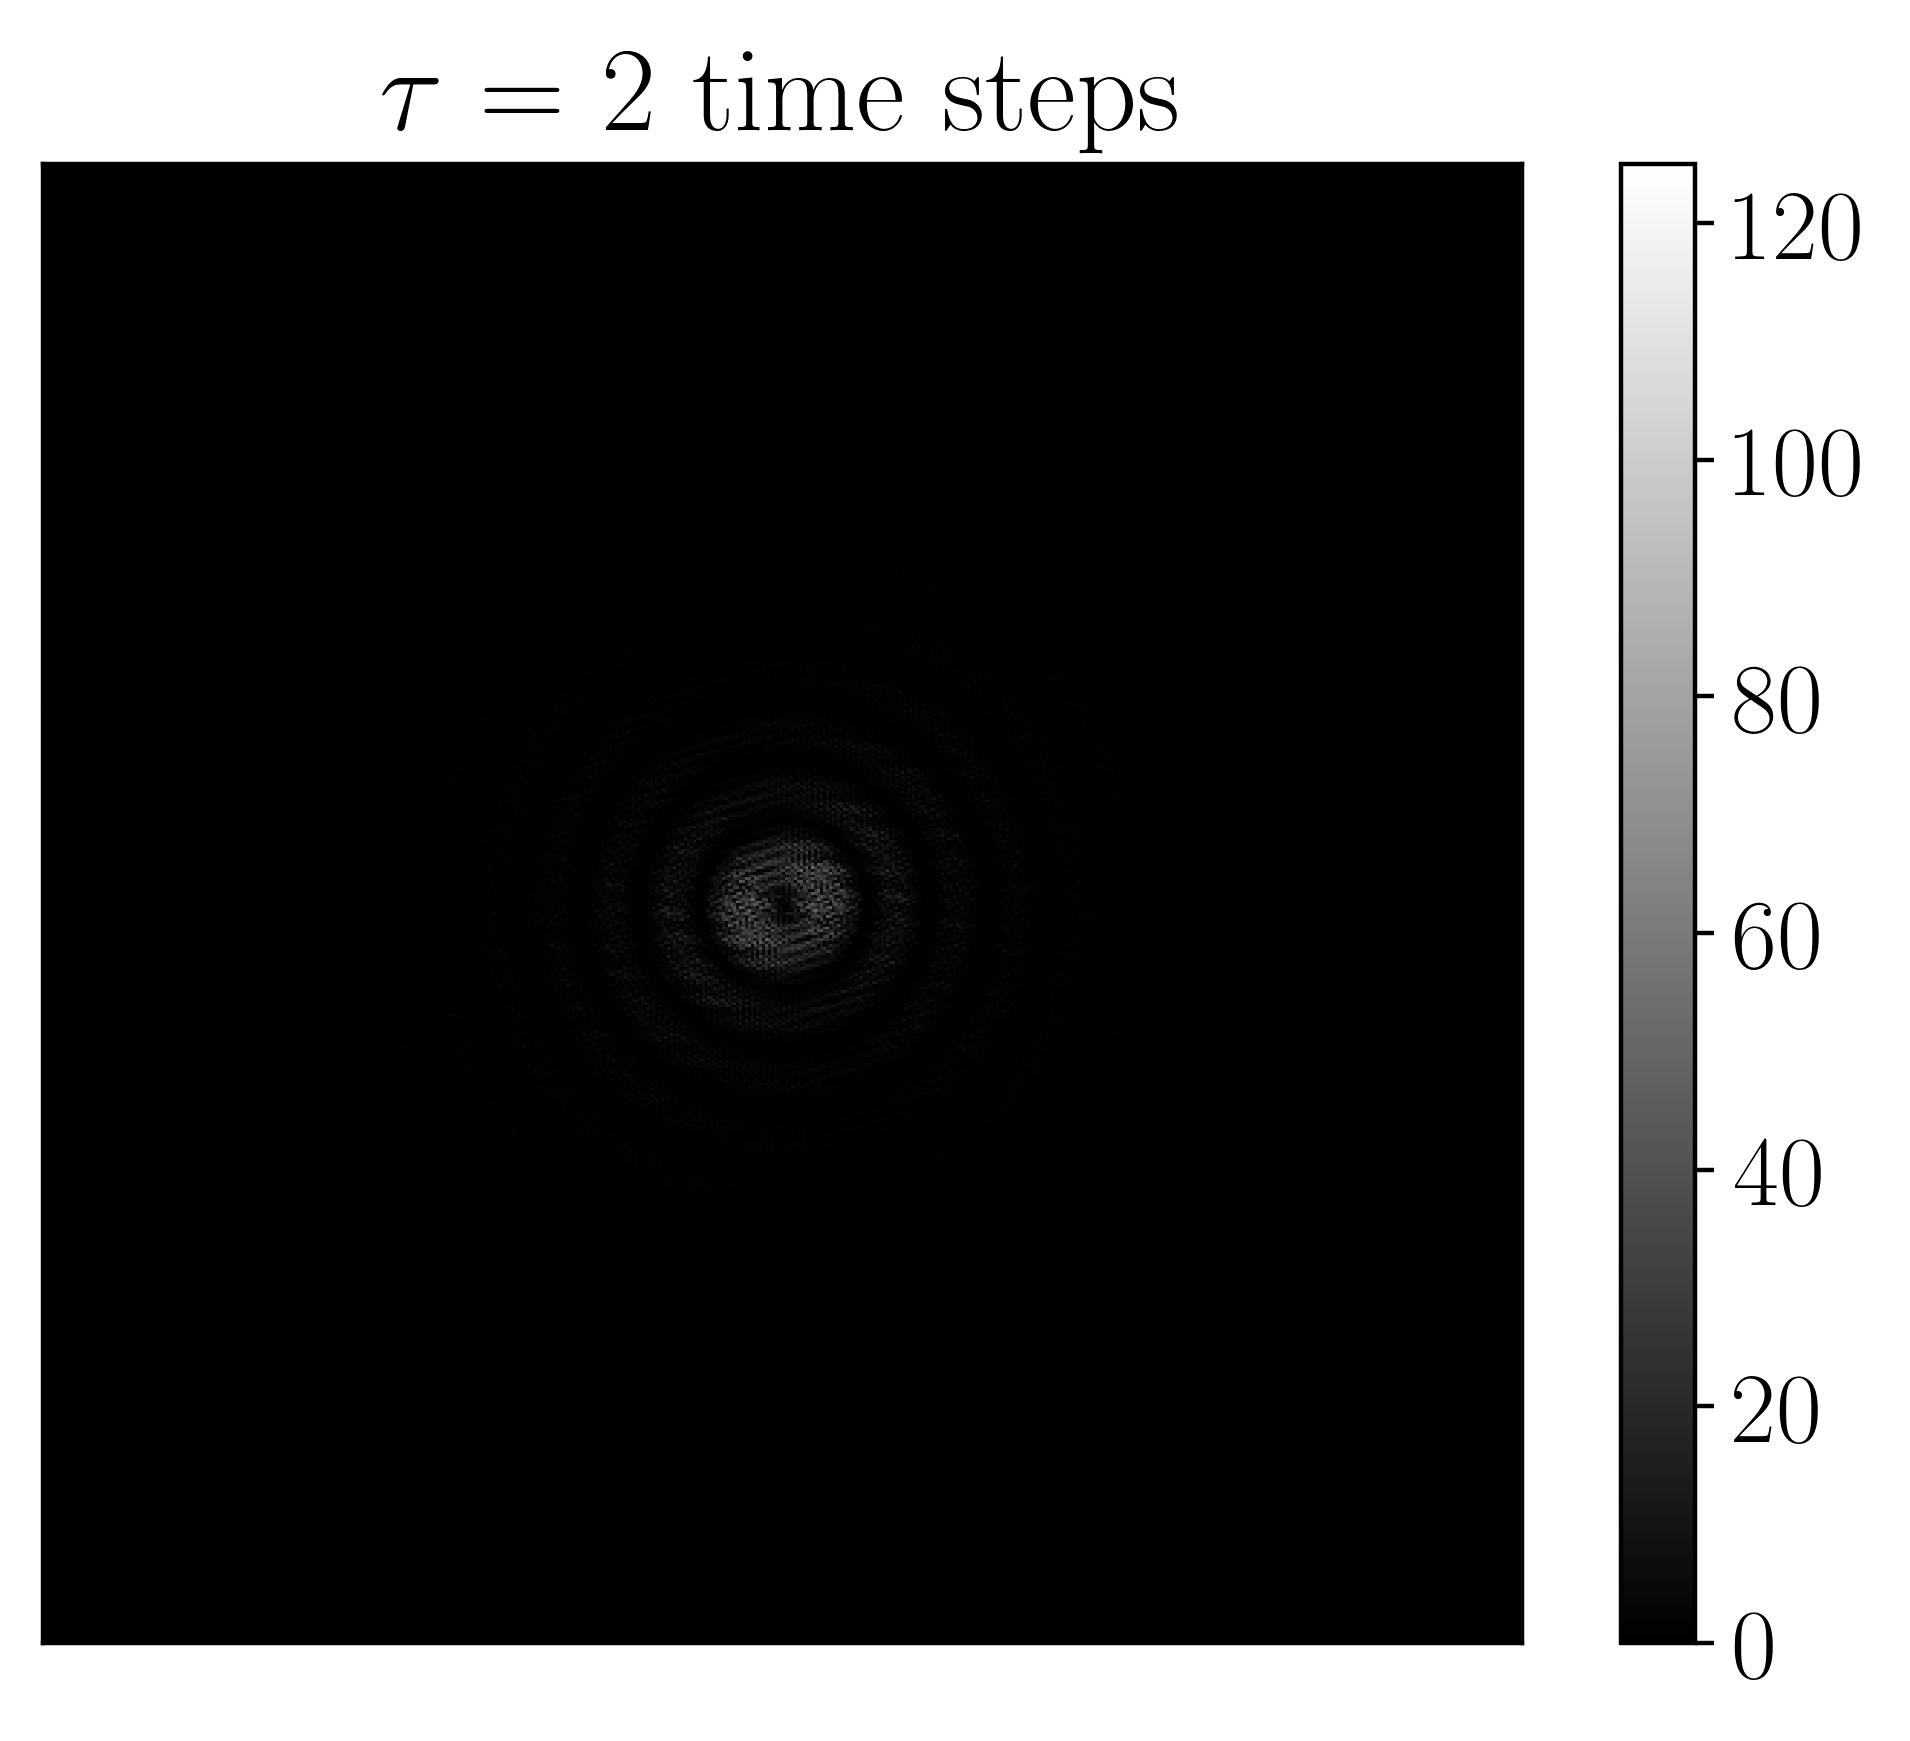
\includegraphics[width=\textwidth]
	{Sources/X-DFA/Mag_Spectrum_d_img_00001.png}}

	\only<3>{
	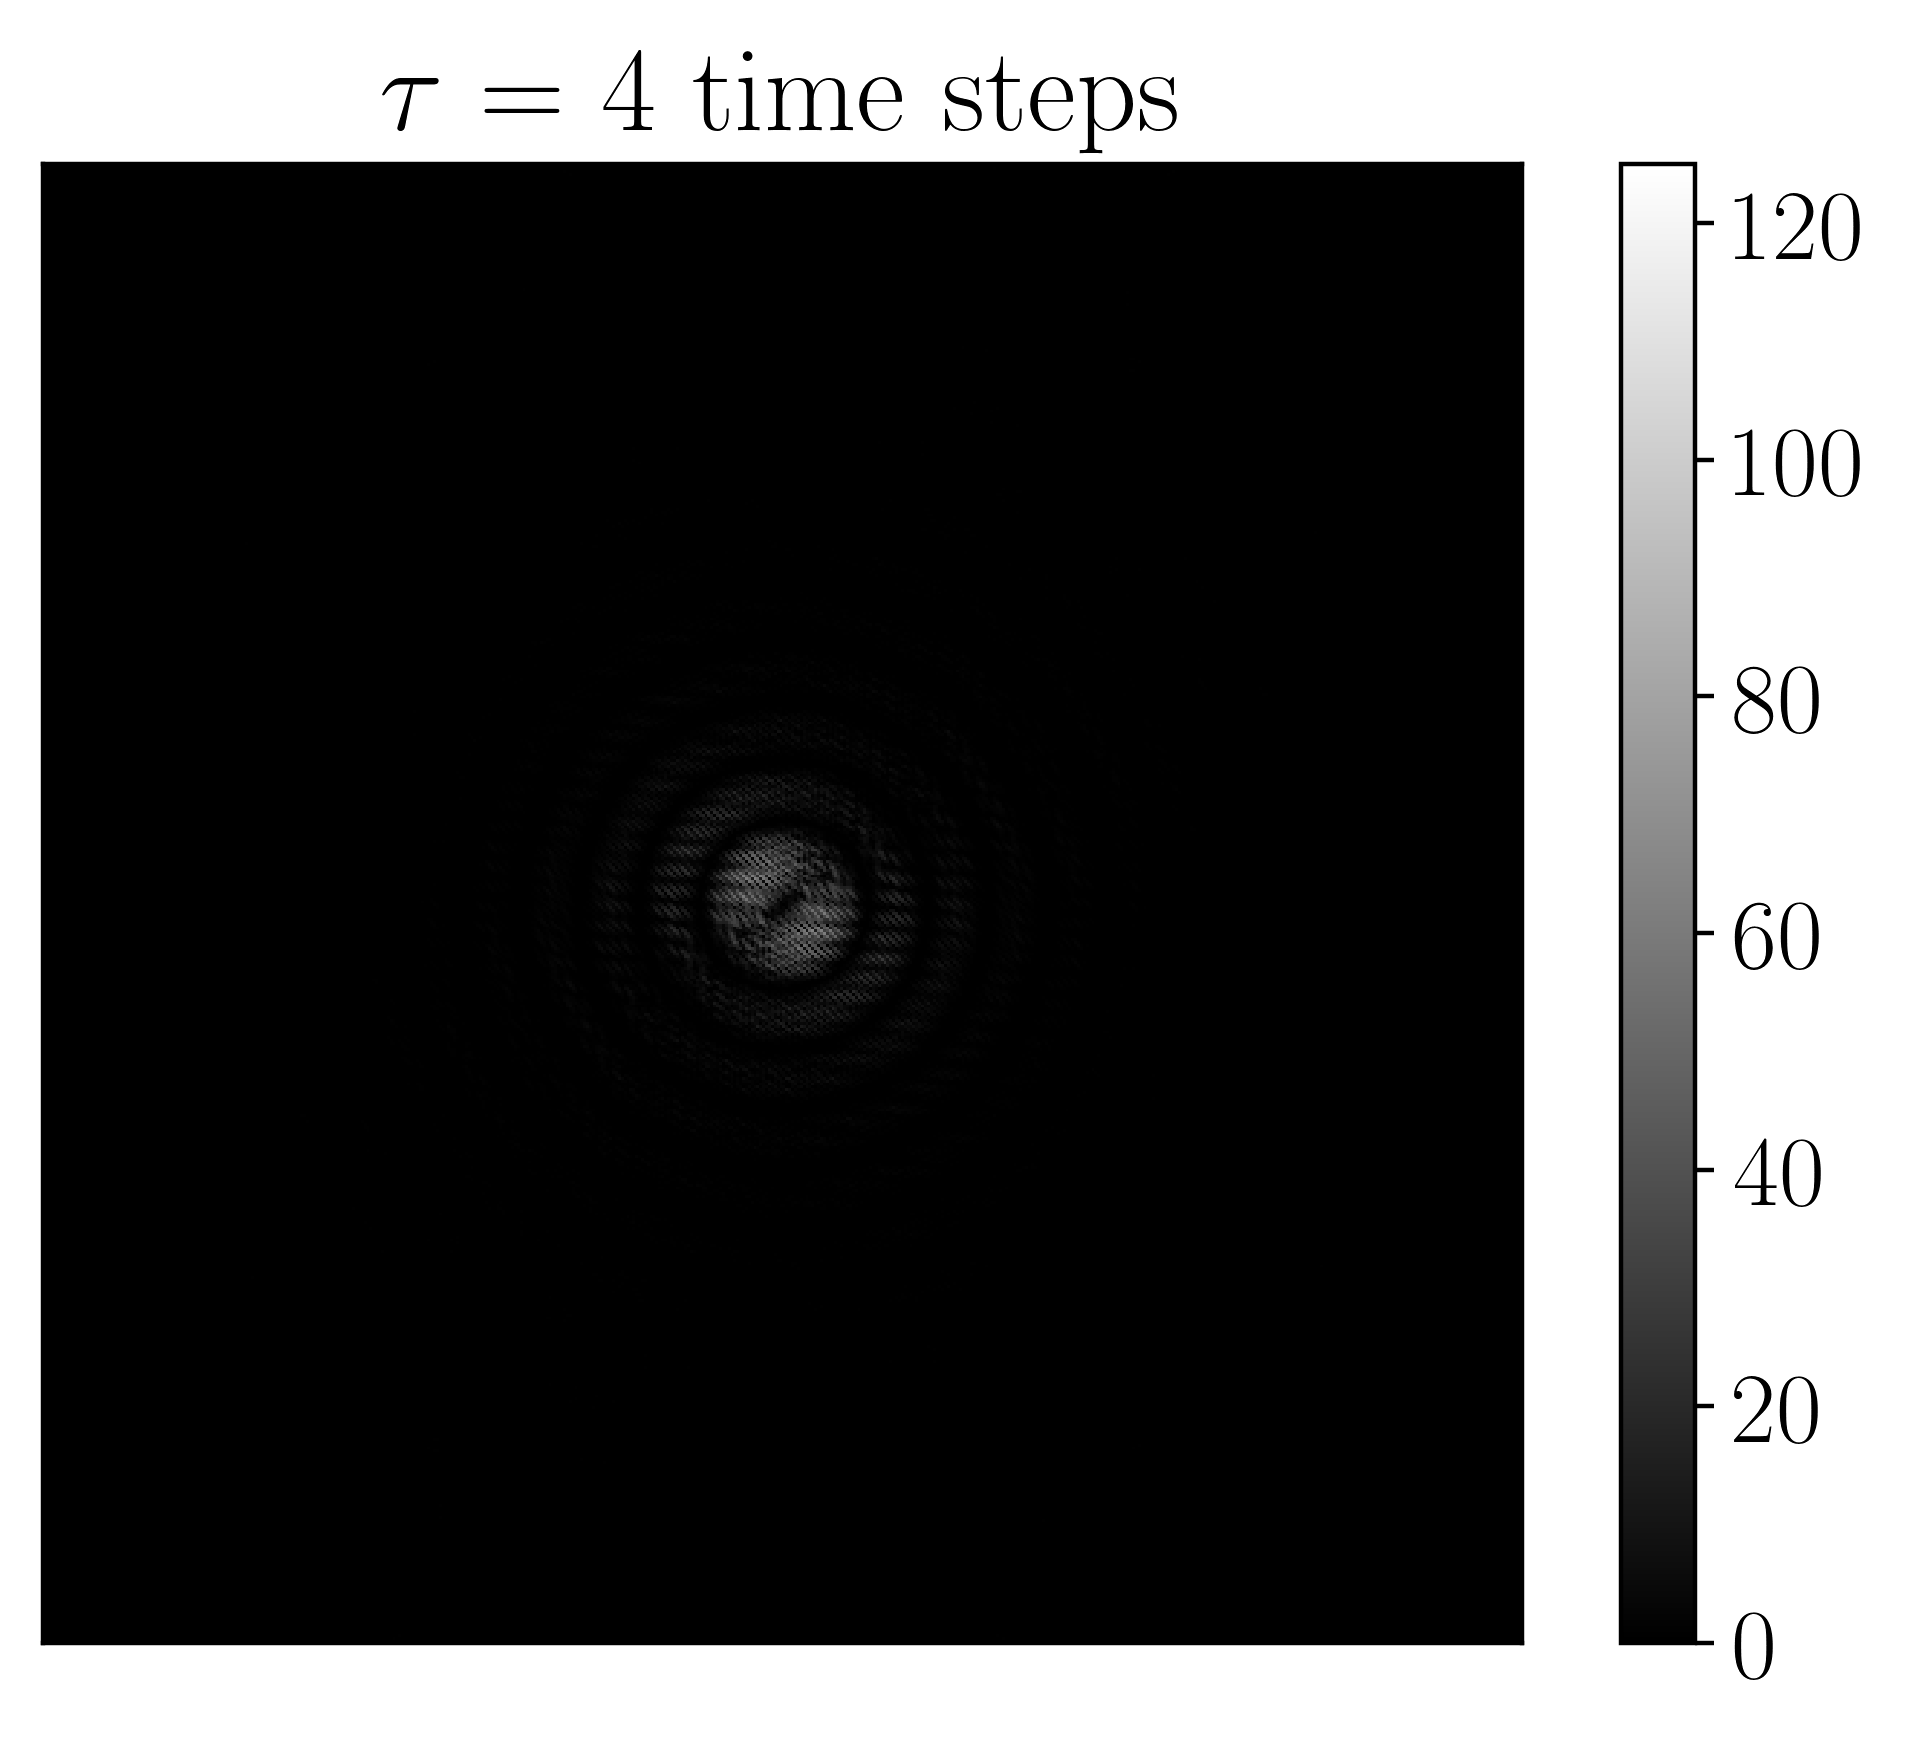
\includegraphics[width=\textwidth]
	{Sources/X-DFA/Mag_Spectrum_d_img_00003.png}}

	\only<4>{
	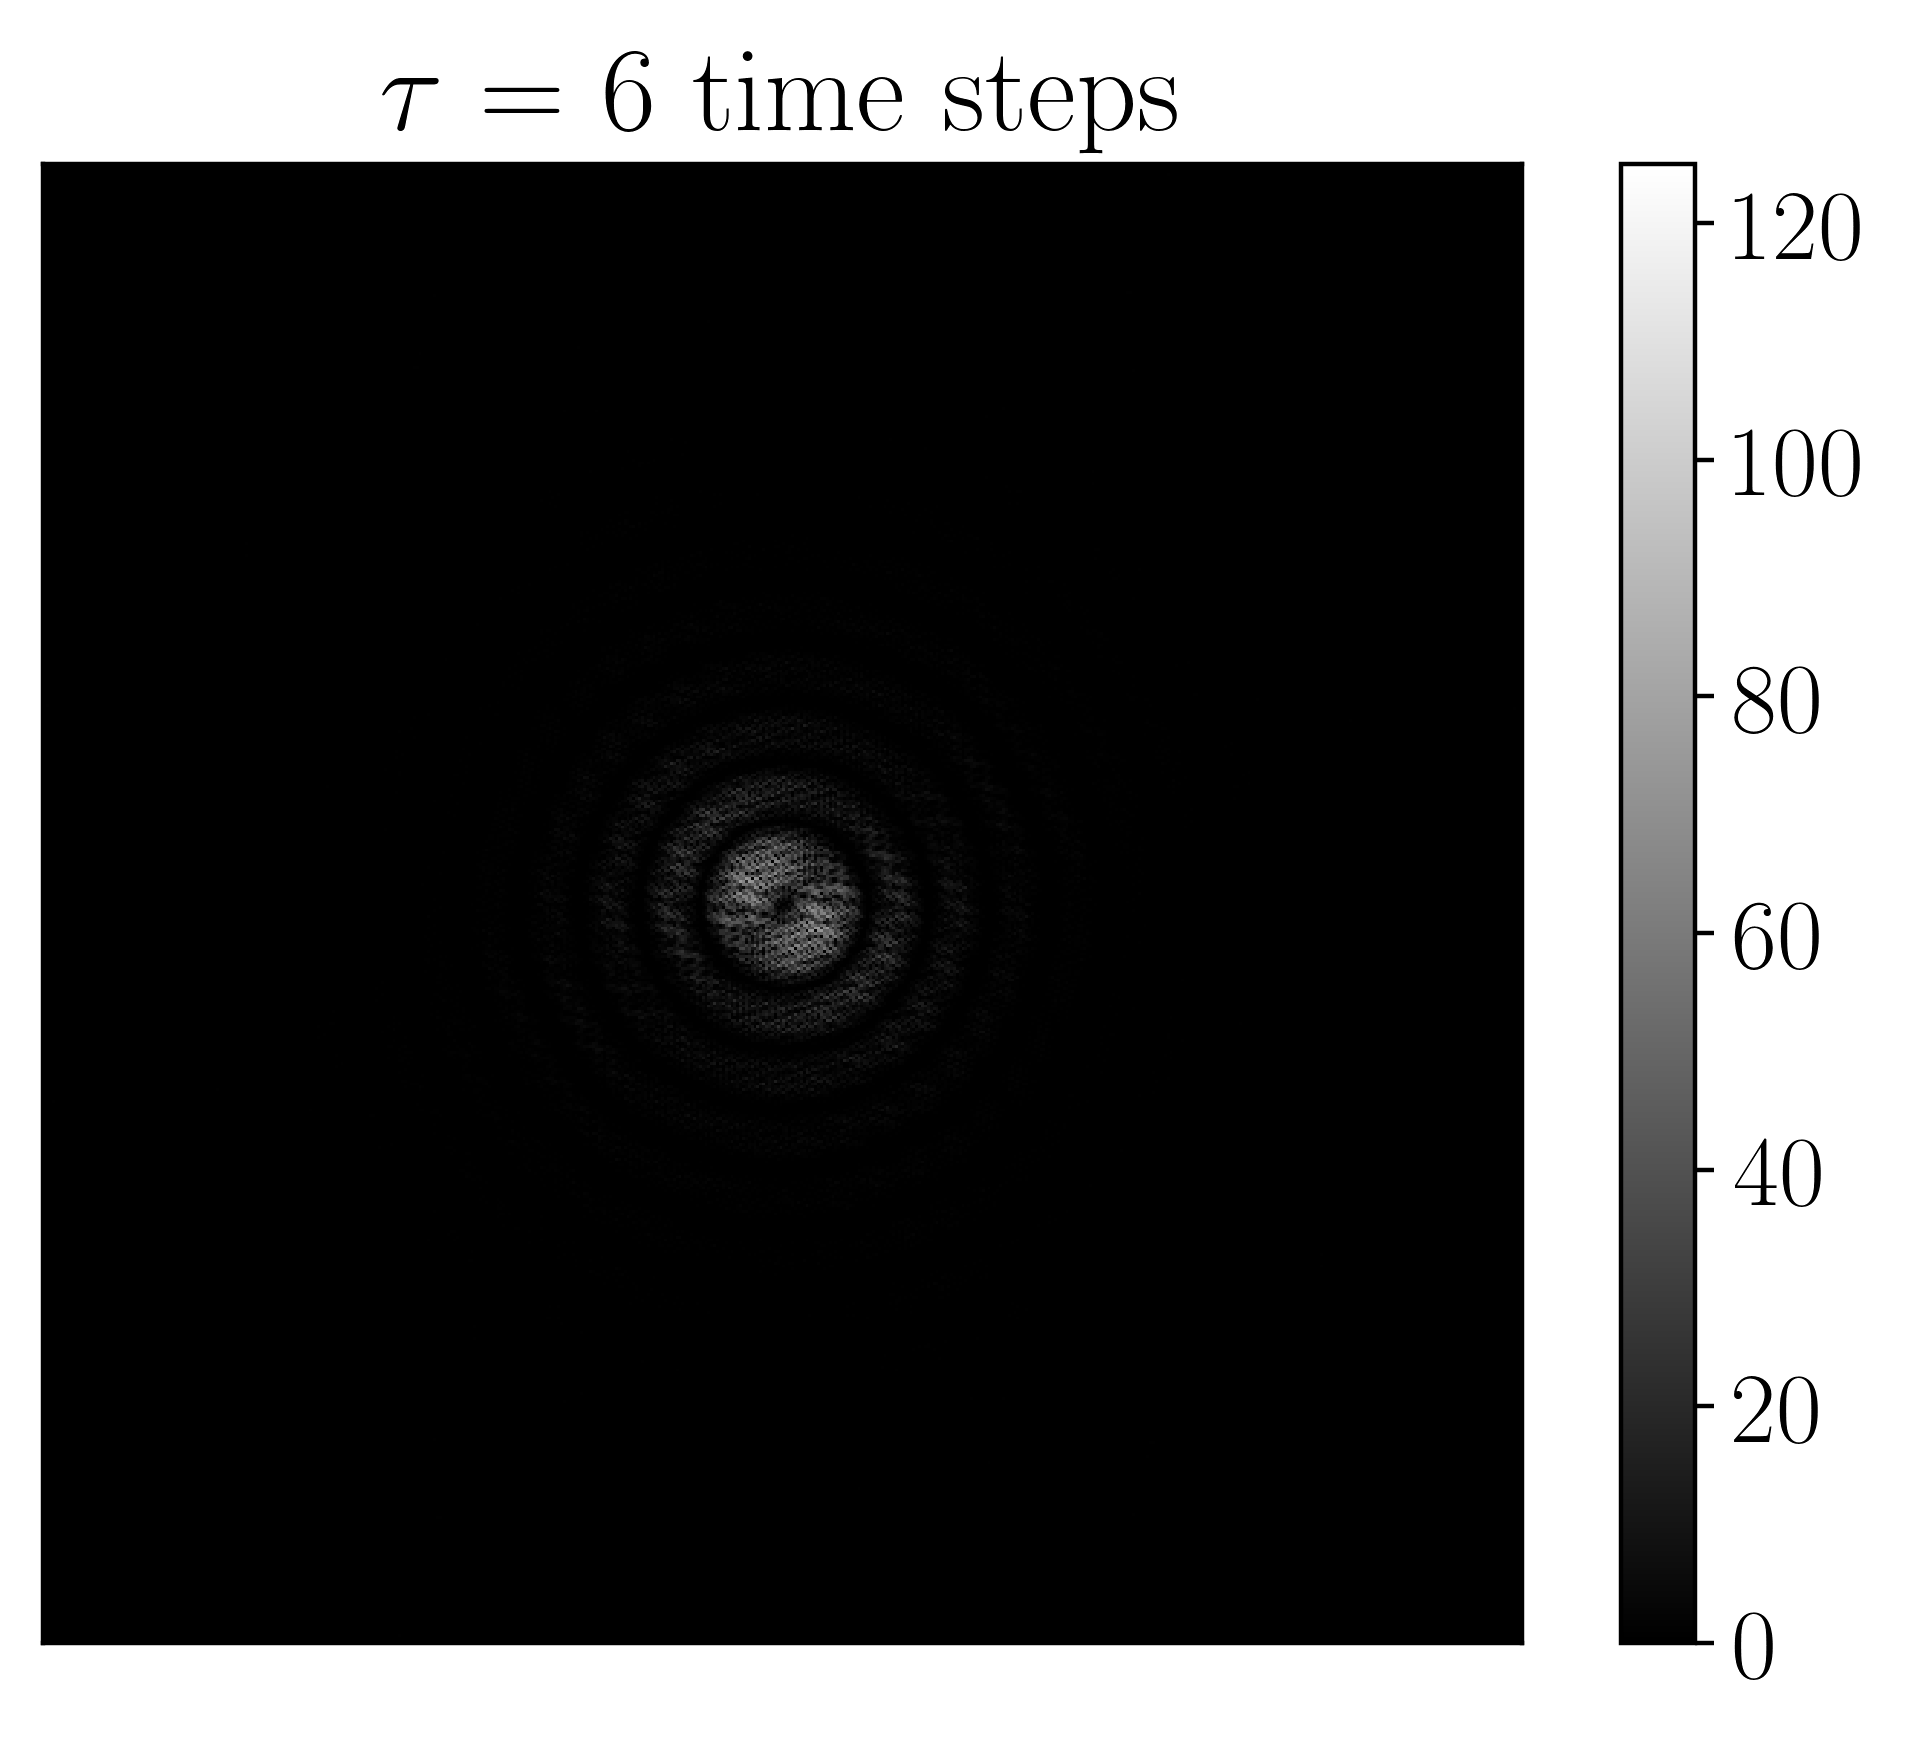
\includegraphics[width=\textwidth]
	{Sources/X-DFA/Mag_Spectrum_d_img_00005.png}}

	\only<5>{
	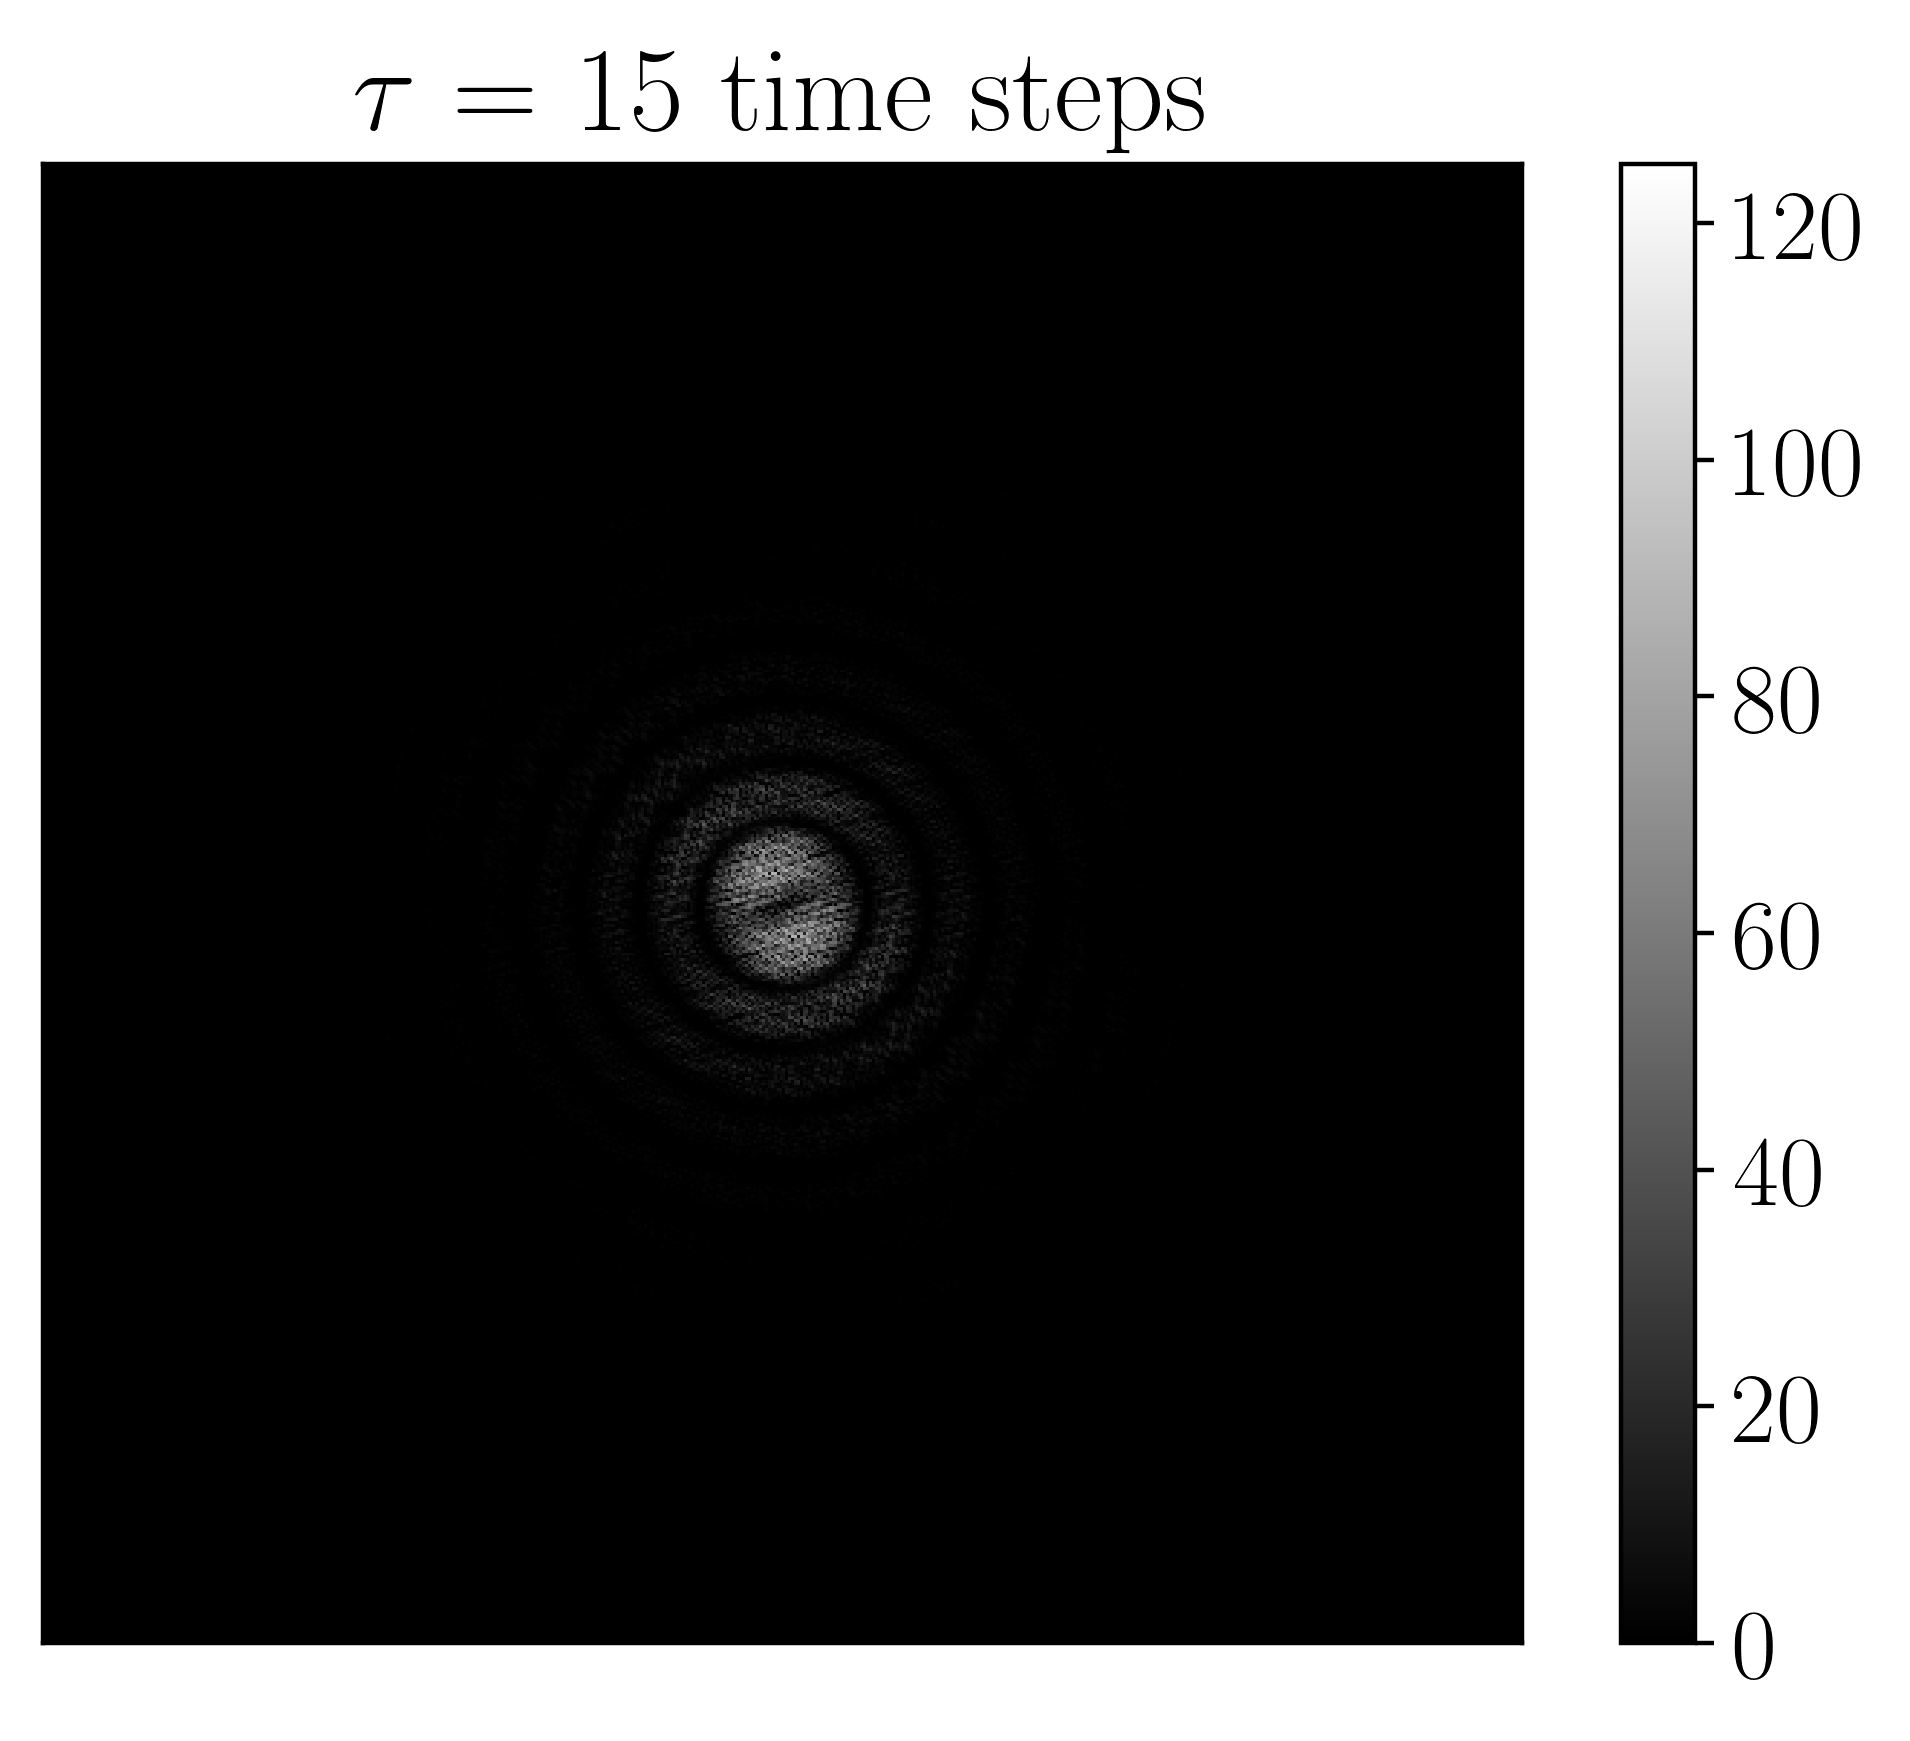
\includegraphics[width=\textwidth]
	{Sources/X-DFA/Mag_Spectrum_d_img_00014.png}}

	\only<6>{
	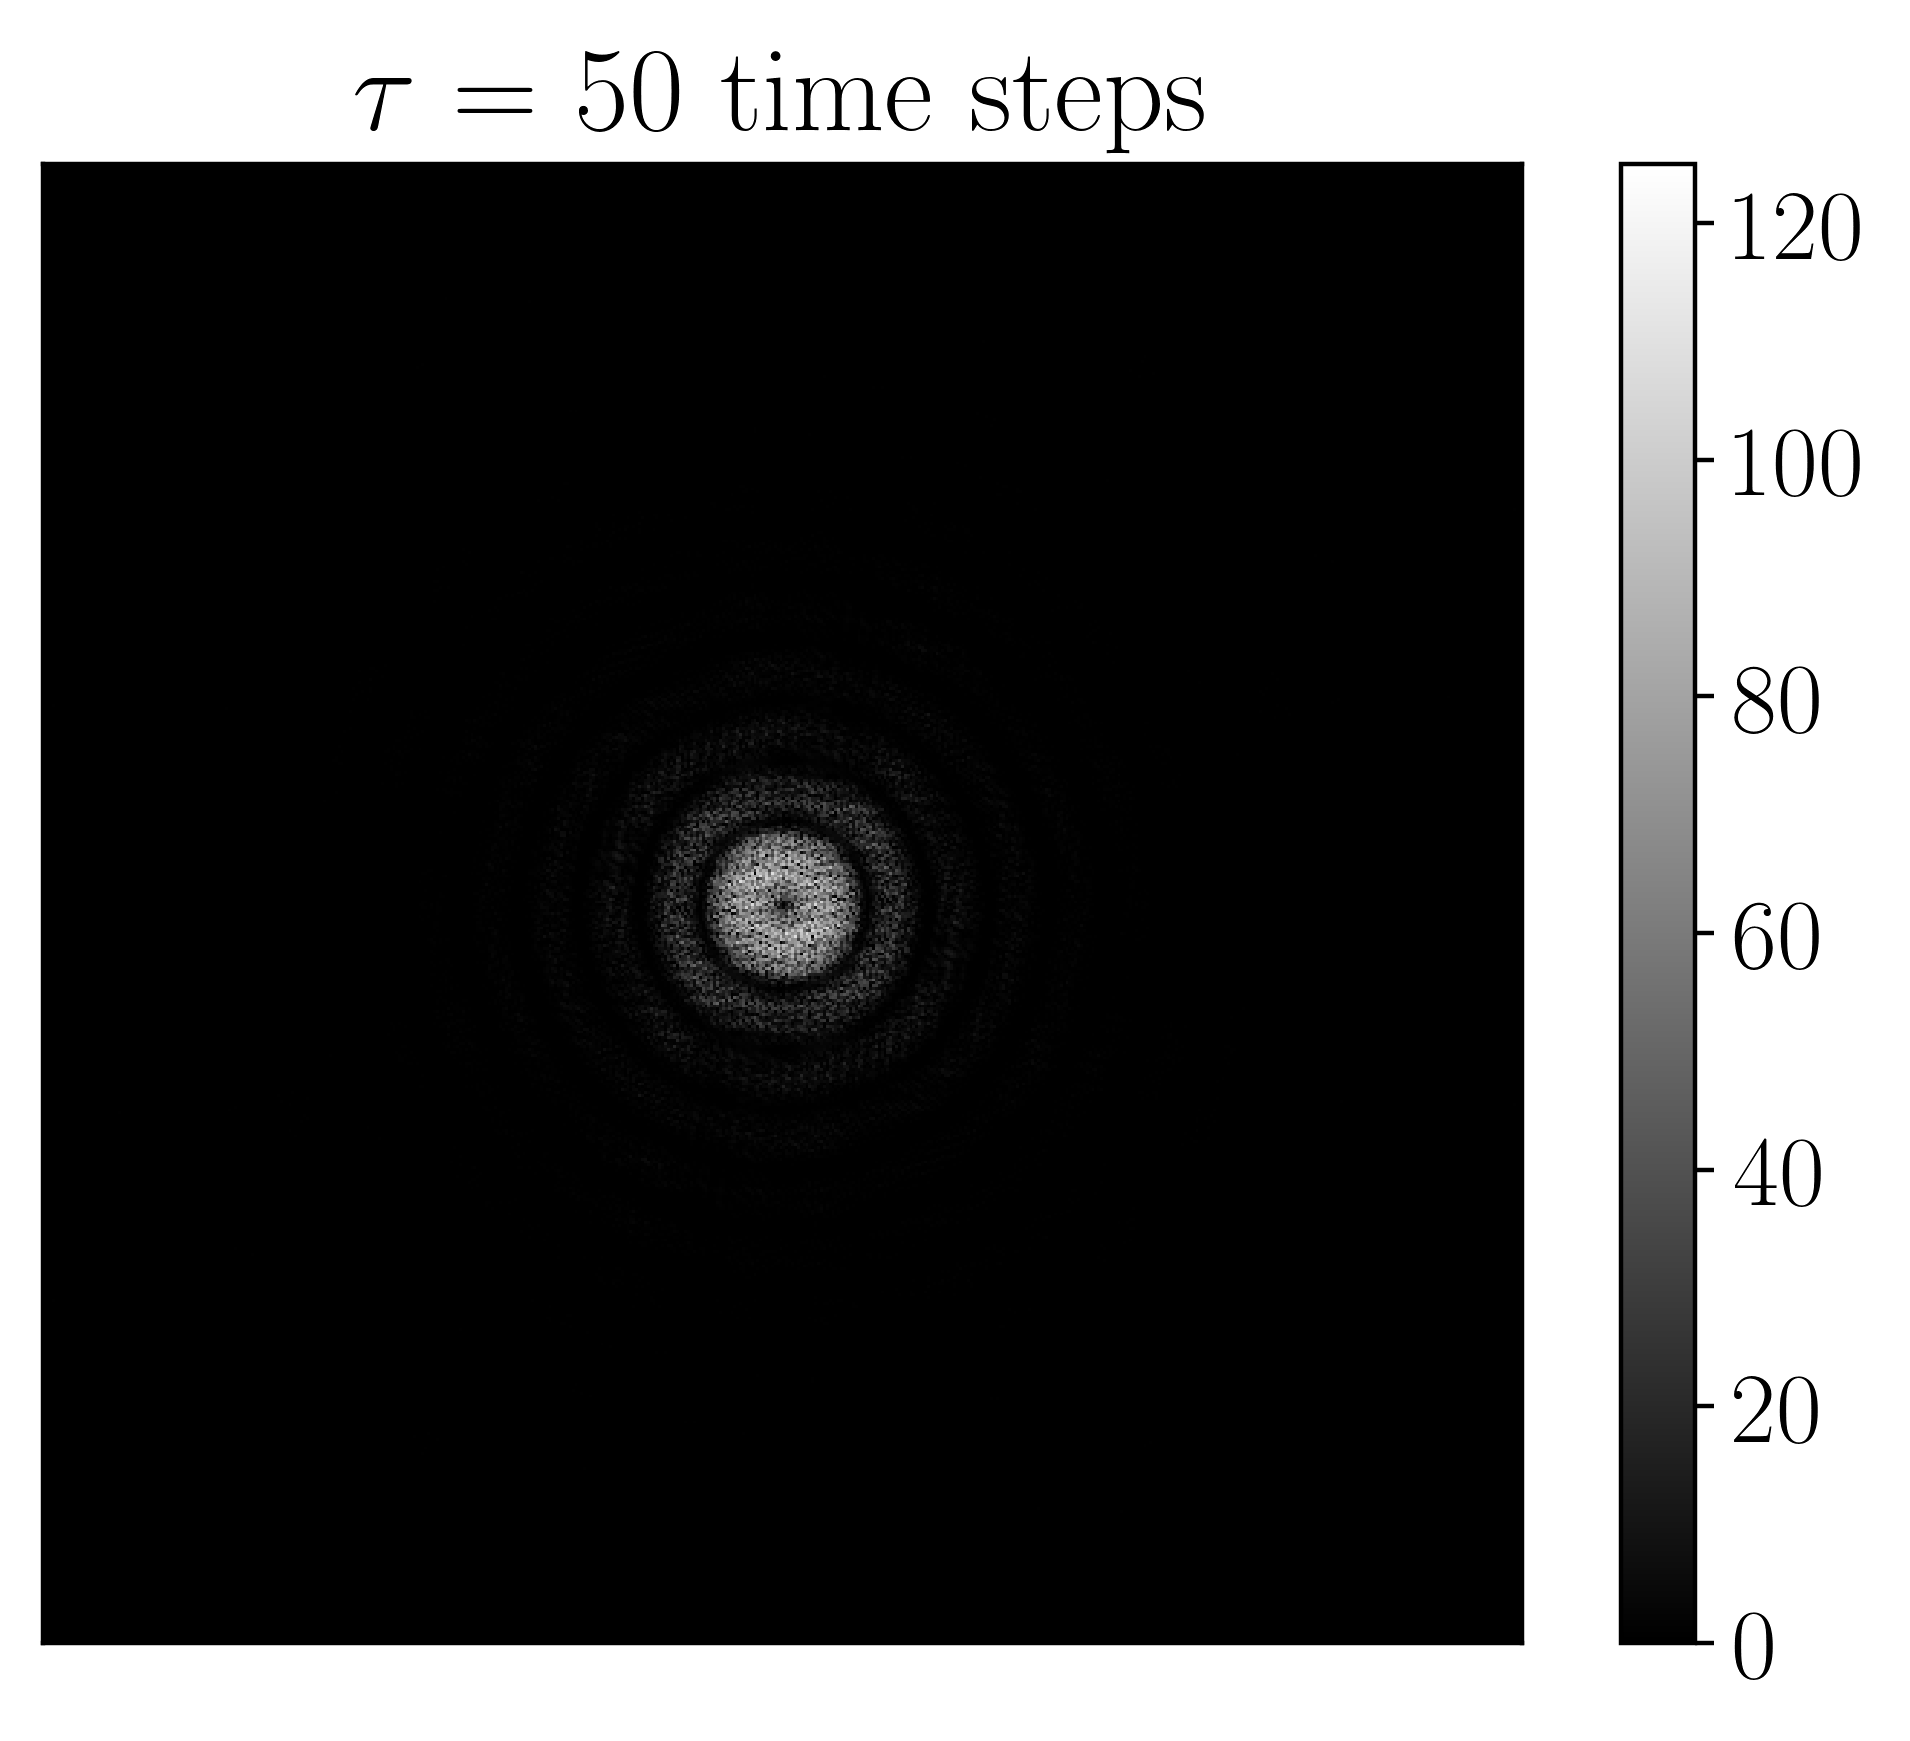
\includegraphics[width=\textwidth]
	{Sources/X-DFA/Mag_Spectrum_d_img_00049.png}}

	\only<7>{
	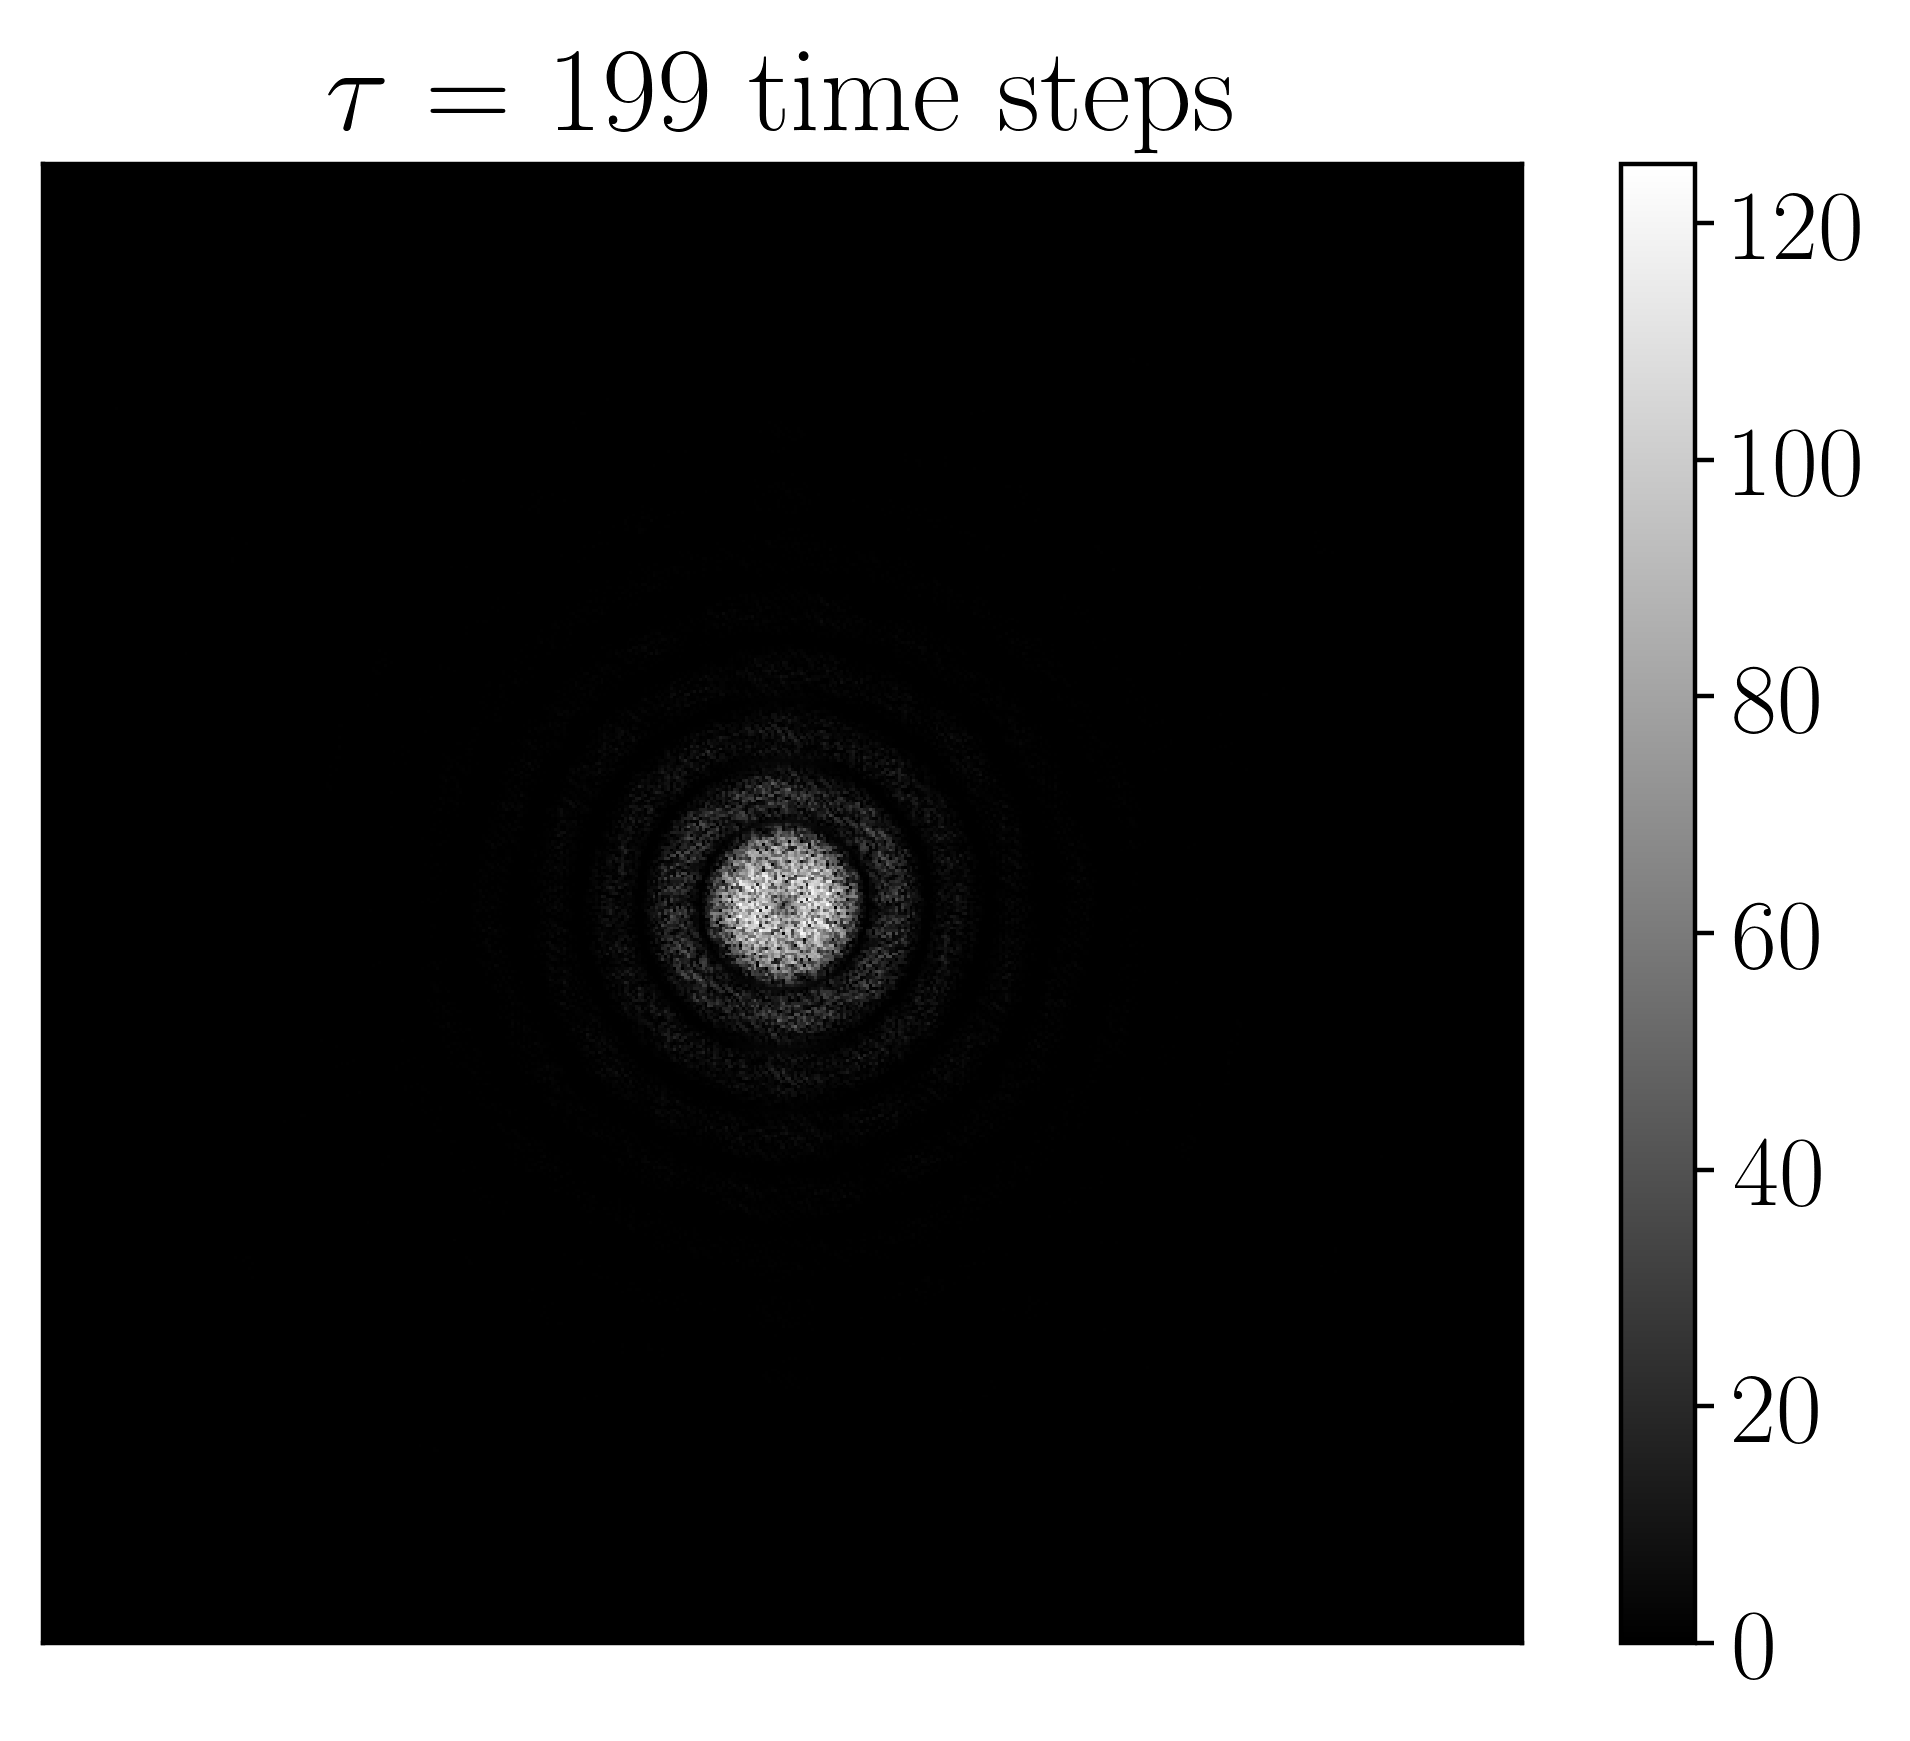
\includegraphics[width=\textwidth]
	{Sources/X-DFA/Mag_Spectrum_d_img_00198.png}}

	\only<8>{
	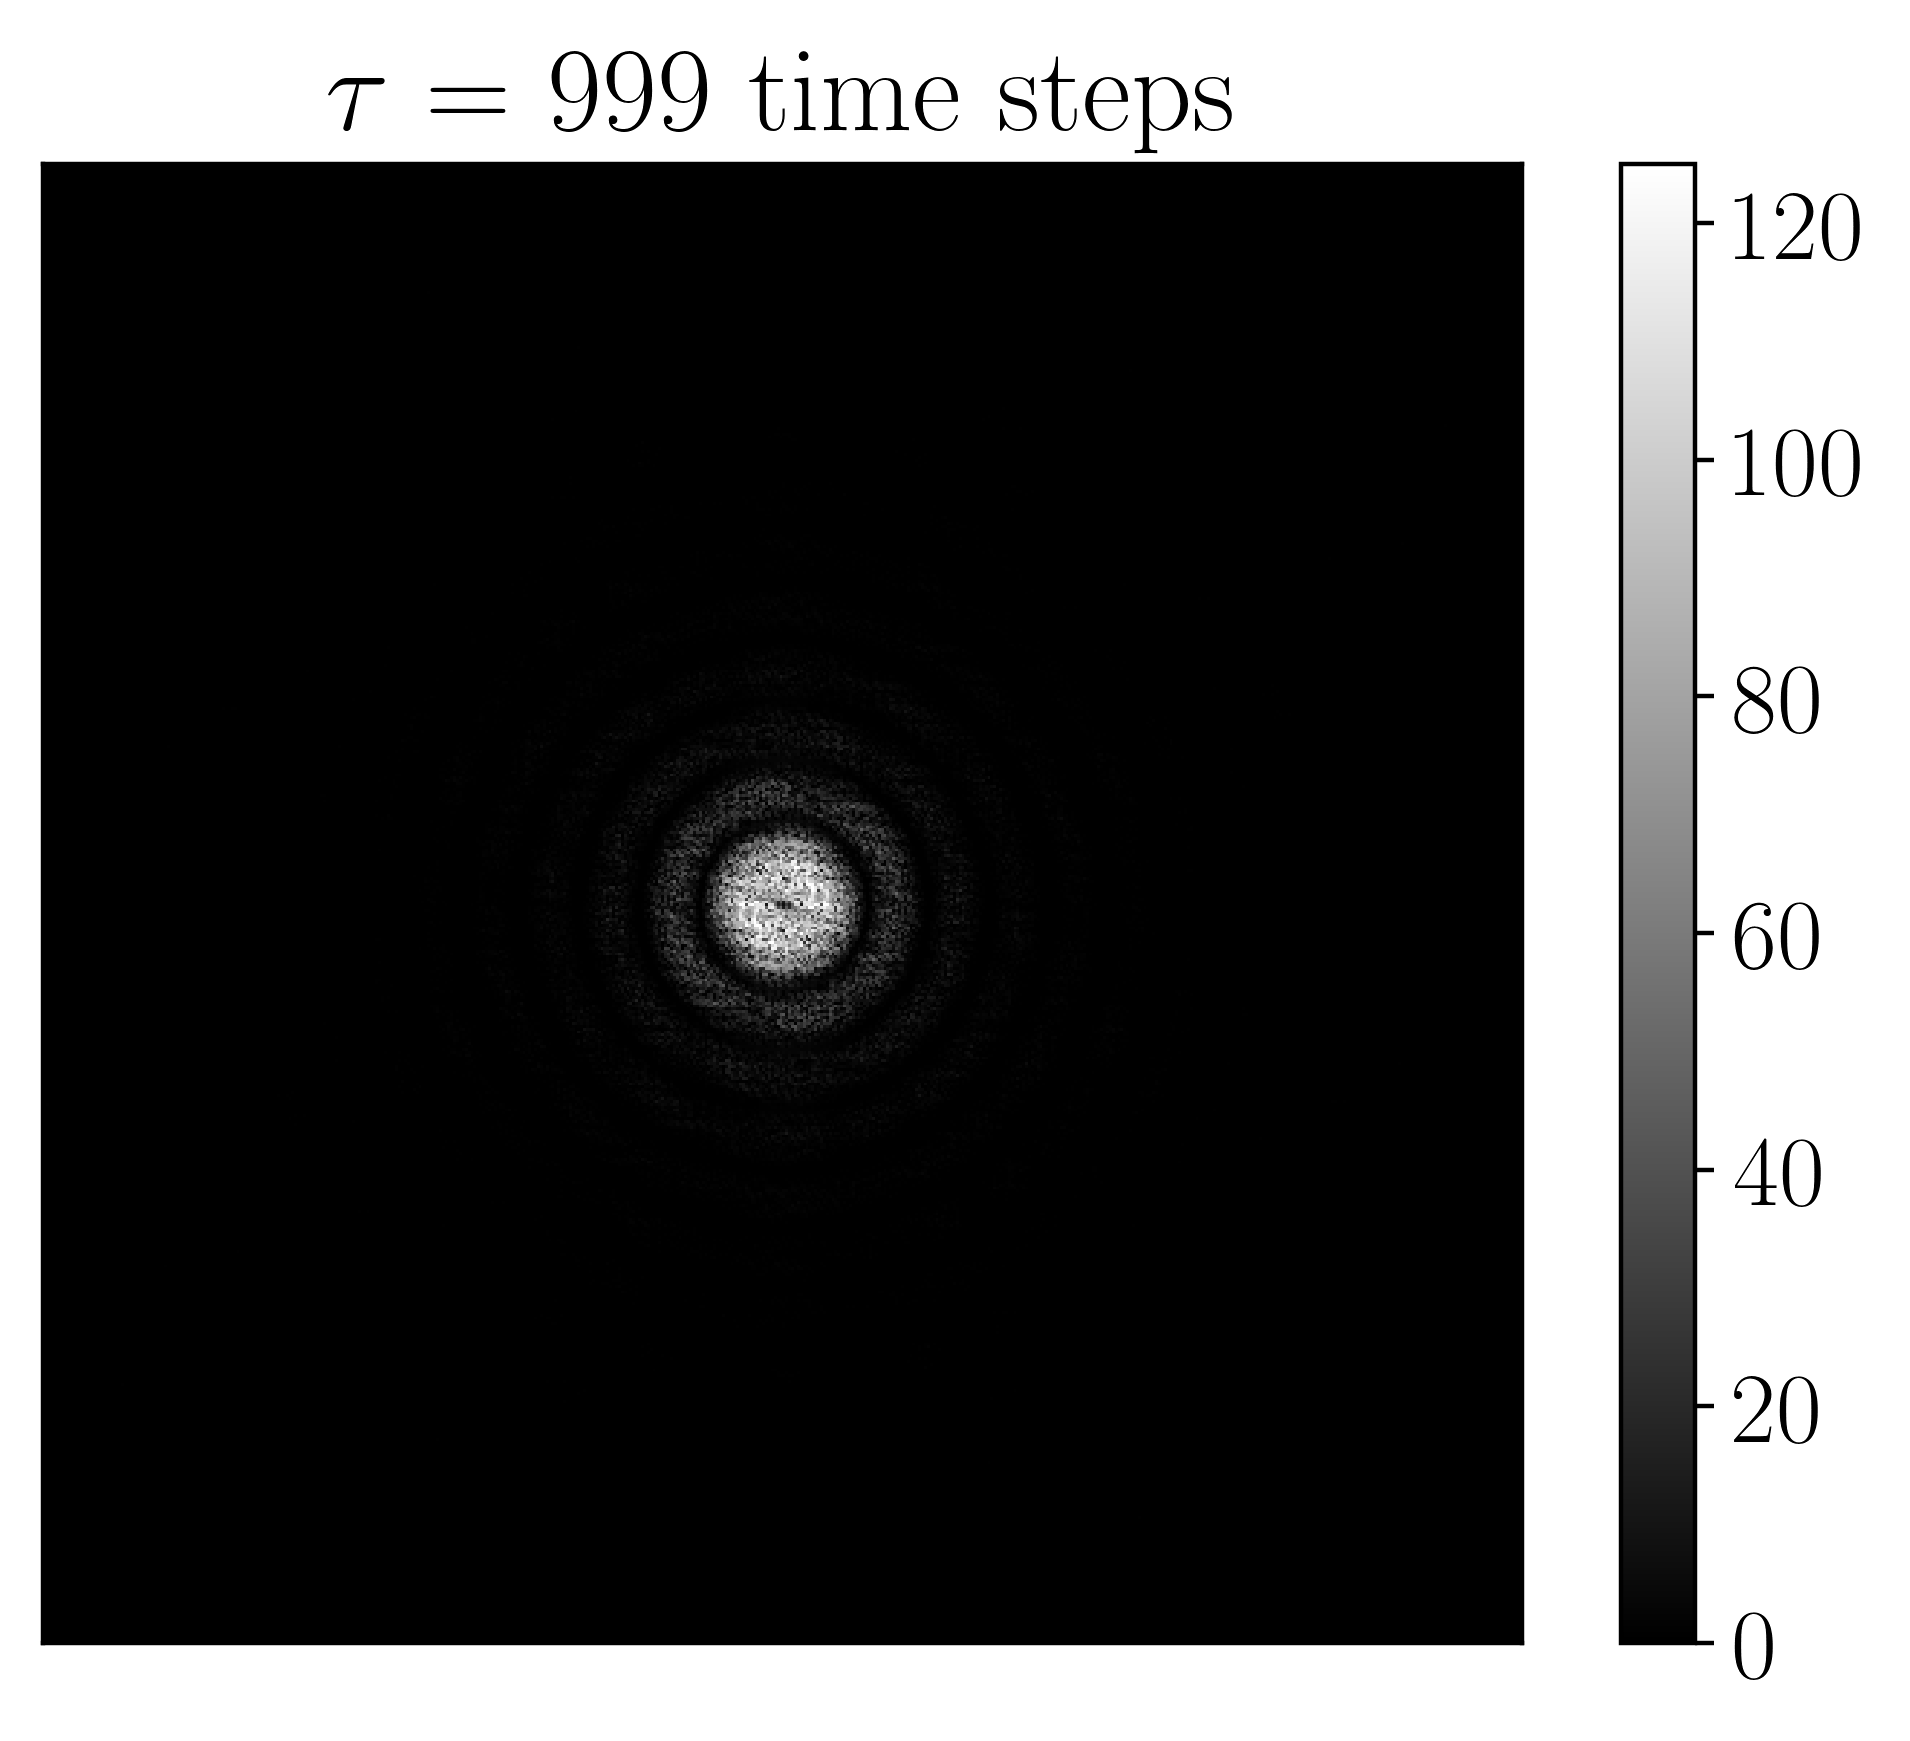
\includegraphics[width=\textwidth]
	{Sources/X-DFA/Mag_Spectrum_d_img_00998.png}}
	\end{textblock}
	
	\begin{textblock}{0.45}(0.5,0.15)
		\centering	
		Time averaging: 
		$D(\mathbf{q},\tau) =  \textcolor{red}{\langle}
		|\mathscr{F}(\Delta I)|^2
		\textcolor{red}{\rangle_t} $\\[0.3cm]
		
		Azimuthal averaging: $D(\mathbf{\textcolor{red}{q}},\tau) \rightarrow D(\textcolor{red}{q},\tau)$ ...
	\end{textblock}

	
	\begin{textblock}{0.5}(0.45,0.35)
	\only<1>{
	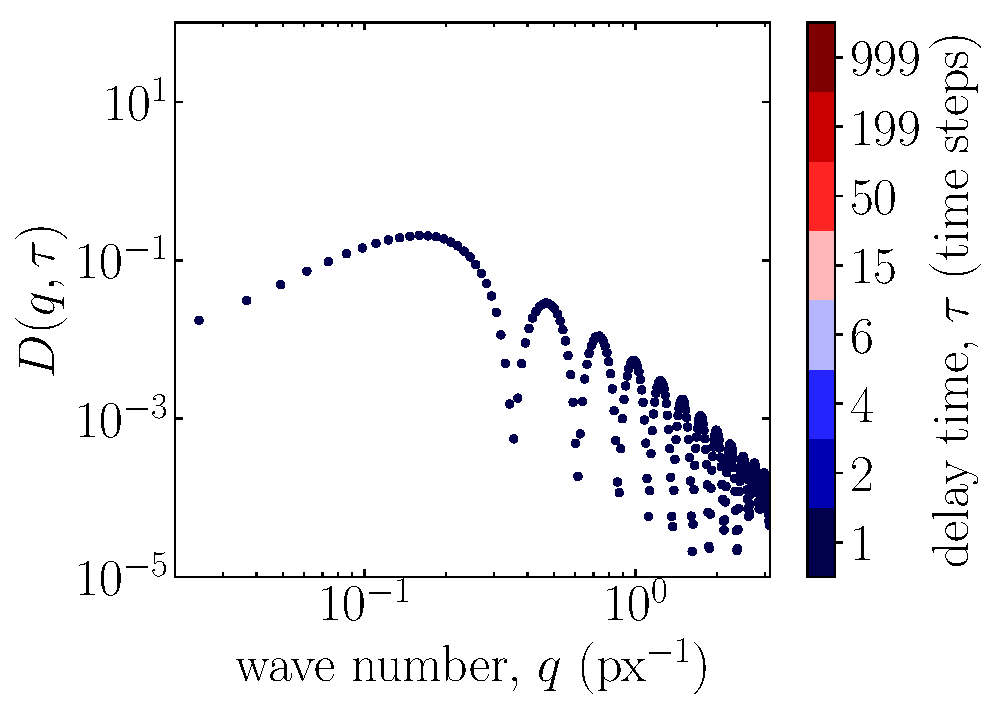
\includegraphics[width=\textwidth]
	{Sources/X-DFA/img_struc_func_vs_q_Ntau1_nPart10.pdf}}
	
	\only<2>{
	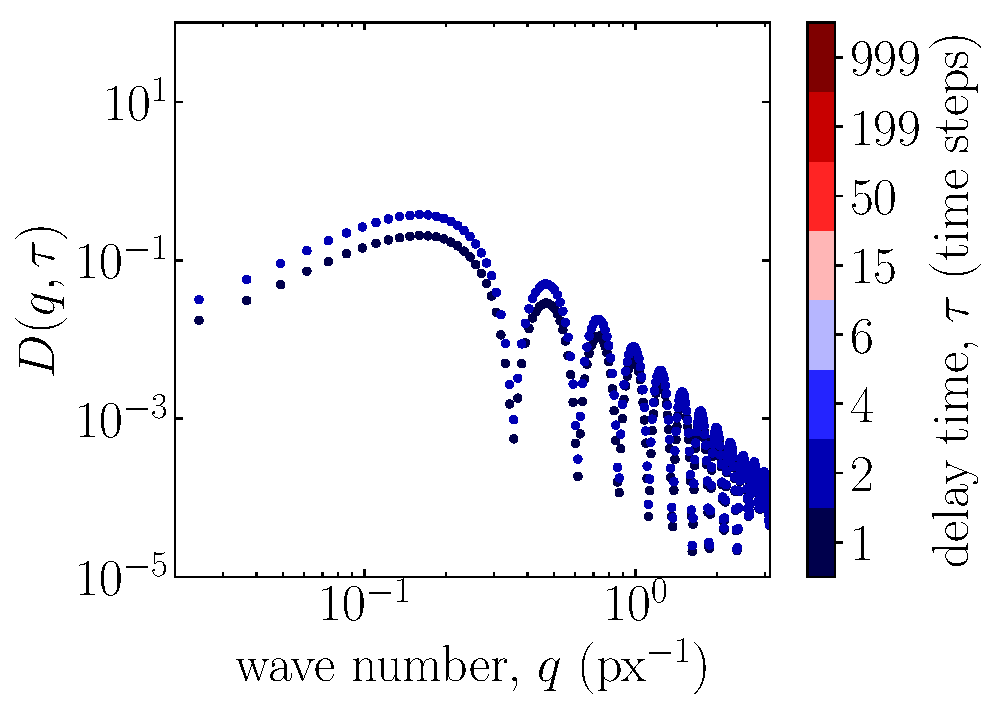
\includegraphics[width=\textwidth]
	{Sources/X-DFA/img_struc_func_vs_q_Ntau2_nPart10.pdf}}

	\only<3>{
	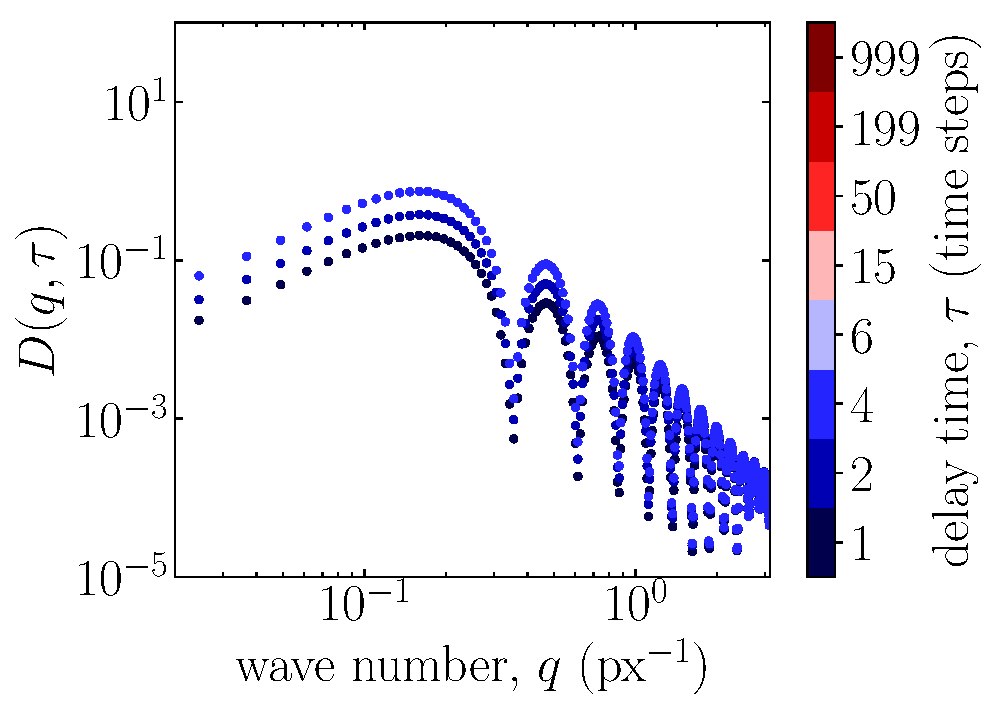
\includegraphics[width=\textwidth]
	{Sources/X-DFA/img_struc_func_vs_q_Ntau4_nPart10.pdf}}

	\only<4>{
	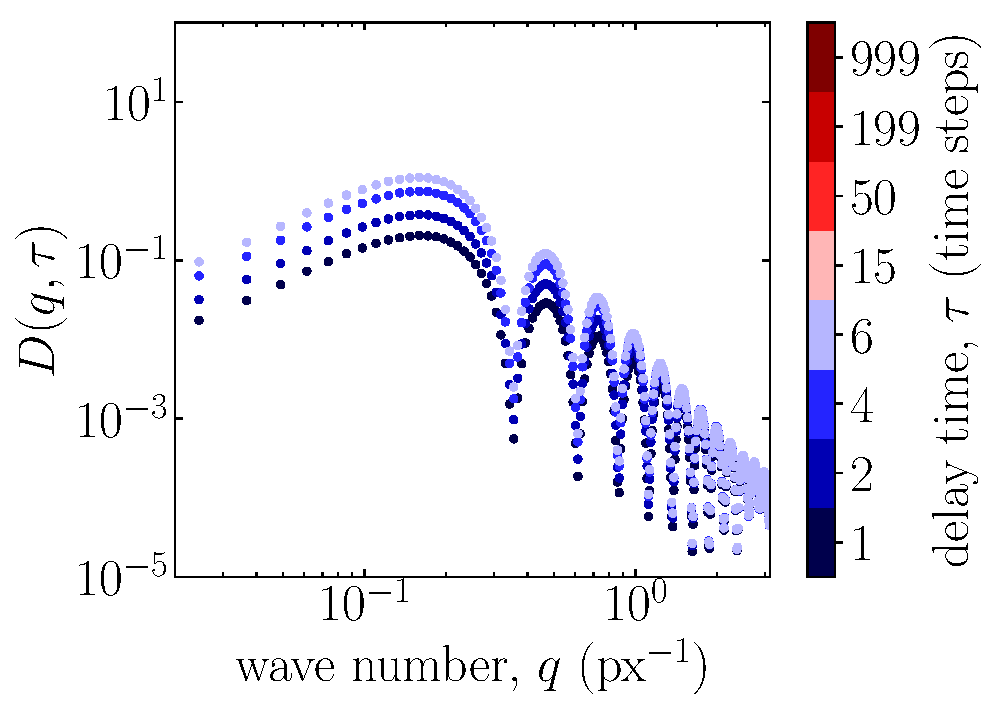
\includegraphics[width=\textwidth]
	{Sources/X-DFA/img_struc_func_vs_q_Ntau6_nPart10.pdf}}

	\only<5>{
	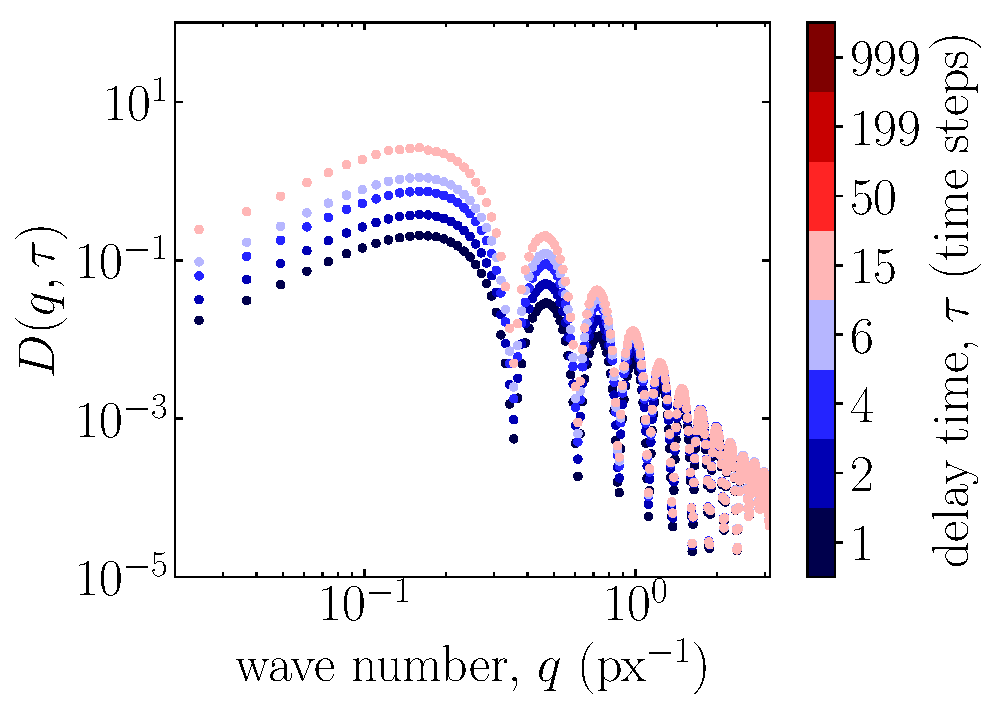
\includegraphics[width=\textwidth]
	{Sources/X-DFA/img_struc_func_vs_q_Ntau15_nPart10.pdf}}

	\only<6>{
	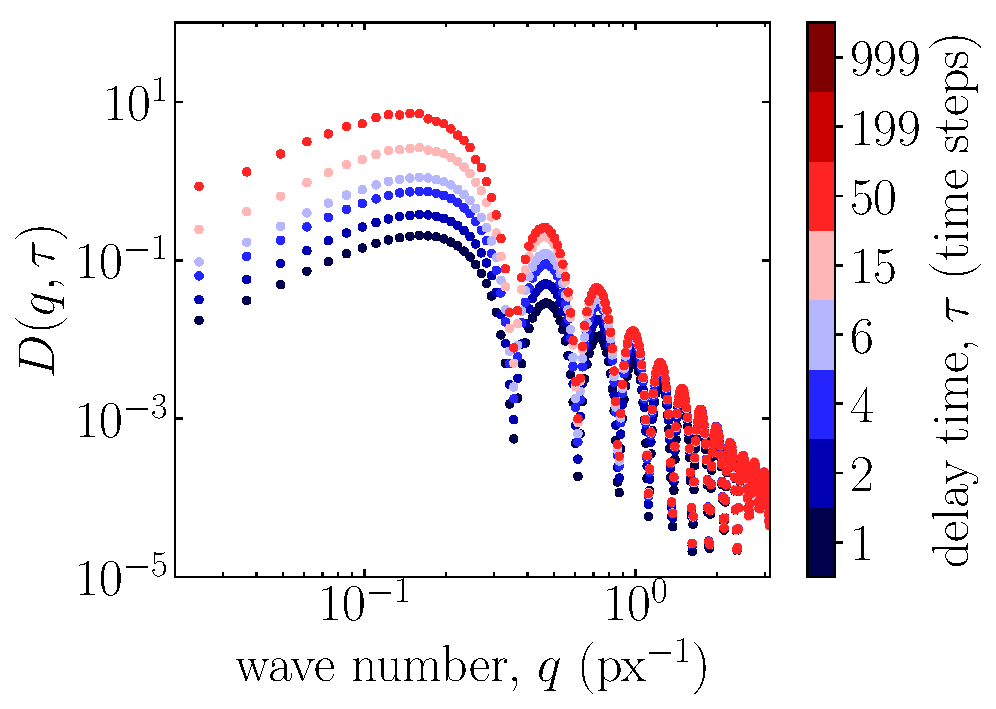
\includegraphics[width=\textwidth]
	{Sources/X-DFA/img_struc_func_vs_q_Ntau50_nPart10.pdf}}

	\only<7>{
	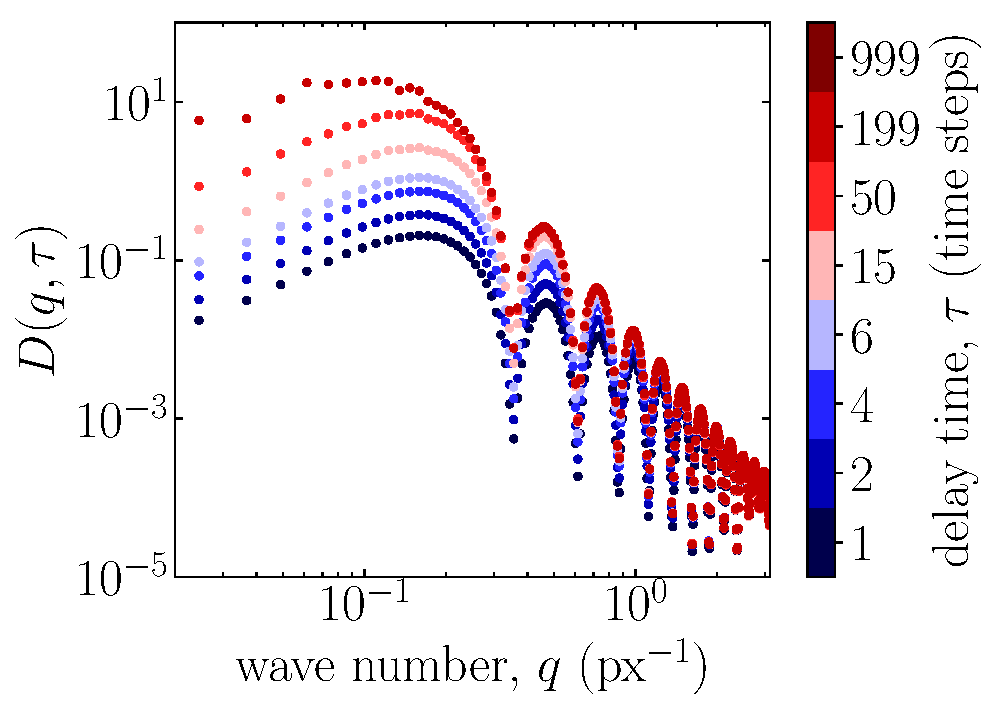
\includegraphics[width=\textwidth]
	{Sources/X-DFA/img_struc_func_vs_q_Ntau199_nPart10.pdf}}

	\only<8>{
	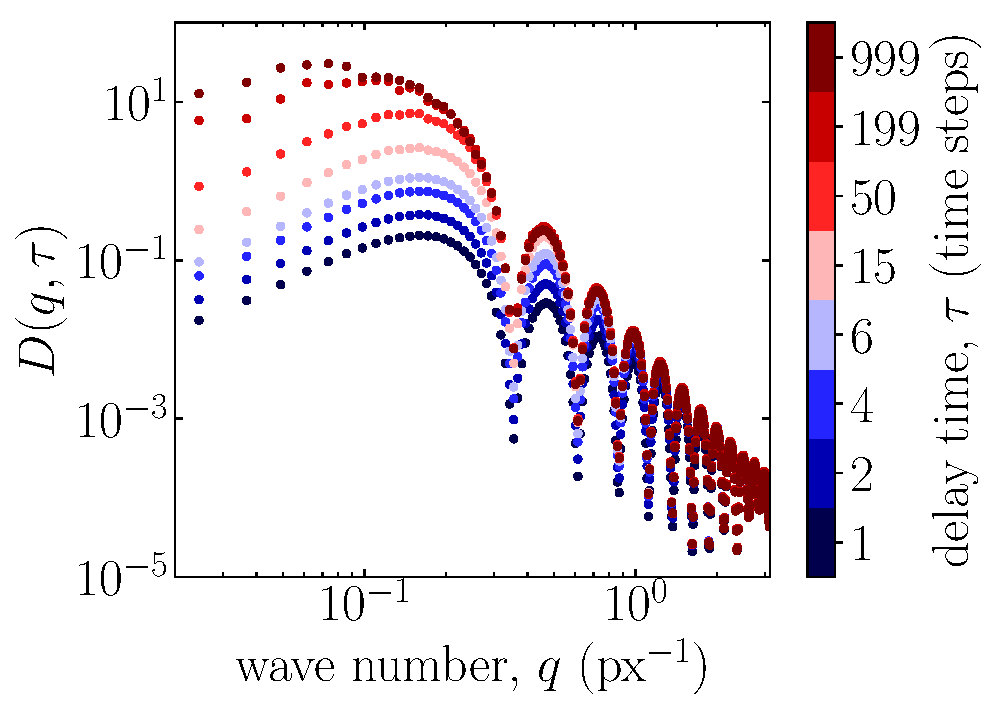
\includegraphics[width=\textwidth]
	{Sources/X-DFA/img_struc_func_vs_q_Ntau999_nPart10.pdf}}
	\end{textblock}

	\begin{textblock}{0.25}(0.05,0.6)
	\centering	
	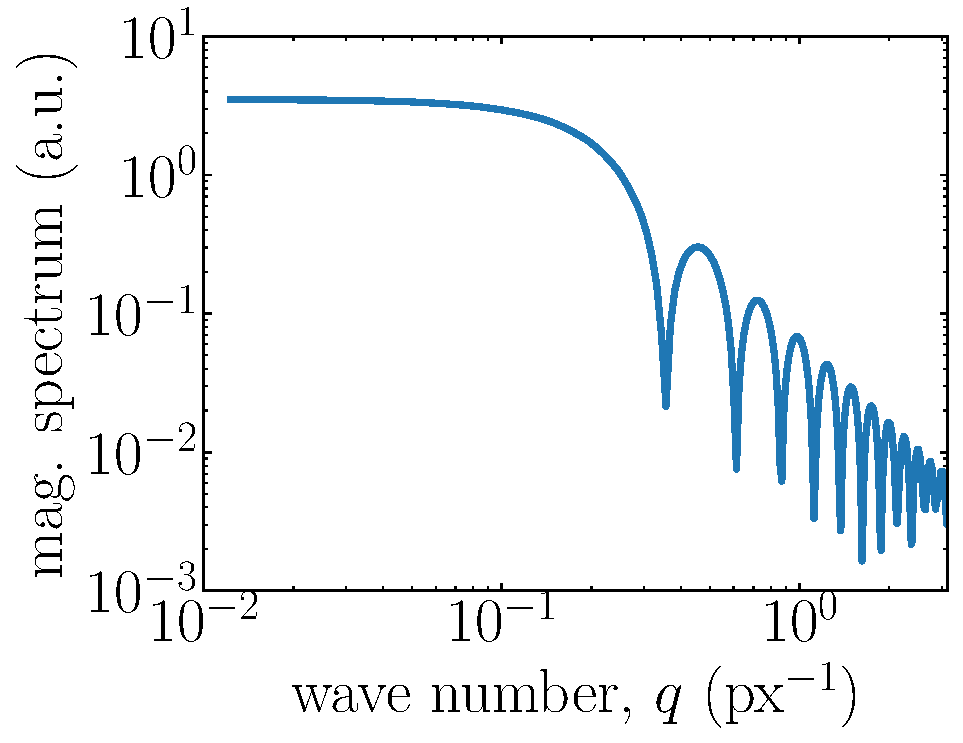
\includegraphics[width=\textwidth]
	{Sources/X-DFA/form_factor.pdf}
	\end{textblock}

	\begin{textblock}{0.06}(0.12,0.7)
	\centering	
	\fbox{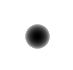
\includegraphics[width=\textwidth]
	{Sources/X-DFA/1Particle_crop_adjust.png}}
	\end{textblock}
}






%%%%%%%%%%%%%%%%%%%%%%%%%%%%%%%%%
%%%%%%%% d(q,tau) vs tau
\begin{frame}
	\begin{tikzpicture}[remember picture,overlay]
	\fill[blue1]
	(current page.north west) rectangle ([xshift=0.52\paperwidth,yshift=0.33\paperheight]current page.west|-{pic cs:end});
	\end{tikzpicture}
	
	\begin{textblock}{0.6}(0.02,0.03)
		\textcolor{white}{
			\Large The image structure function $D(q, \tau)$}
	\end{textblock}

	\begin{textblock}{0.44}(0.02,0.1)
	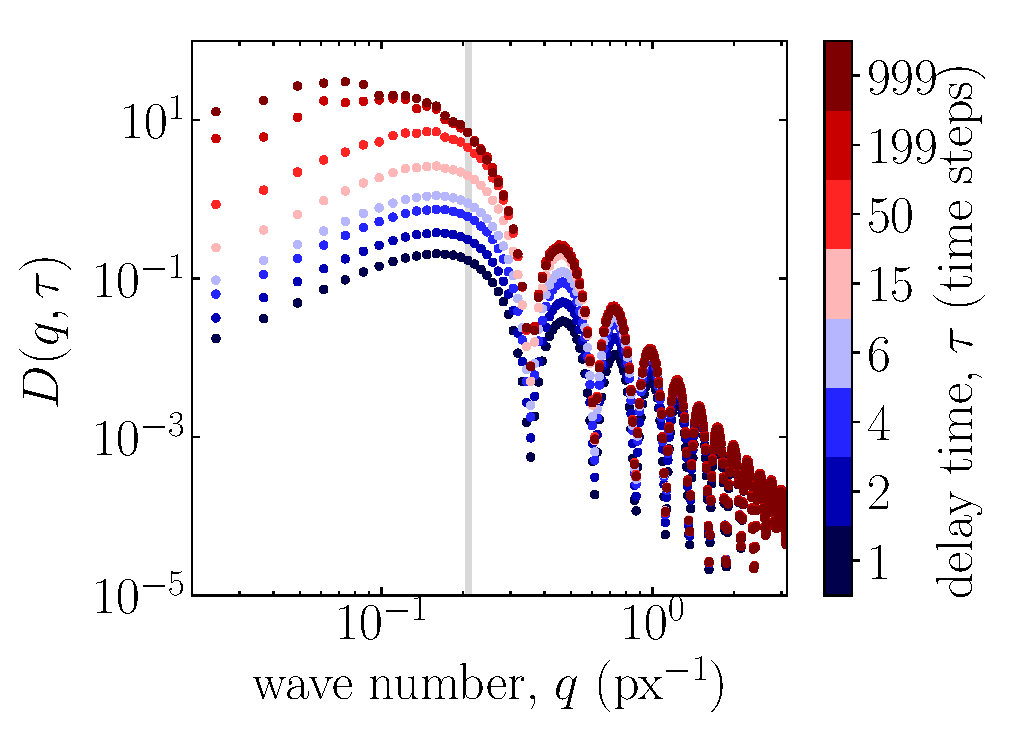
\includegraphics[width=\textwidth]
	{Sources/X-DFA/img_struc_func_vs_q_multiple_tau_simulations_nPart10Marker.eps}
	\end{textblock}

	\begin{textblock}{0.44}(0.52,0.1)
	\only<1>{
	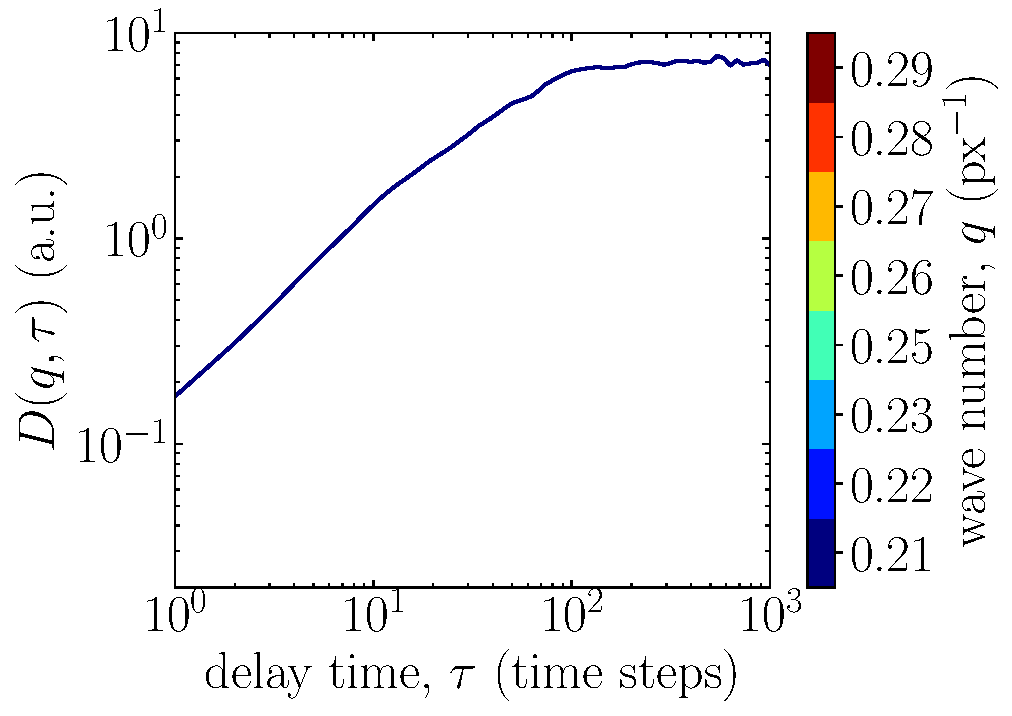
\includegraphics[width=\textwidth]
	{Sources/X-DFA/img_struc_func_vs_tau_q_range_000simulations10.pdf}}

	\only<2>{
	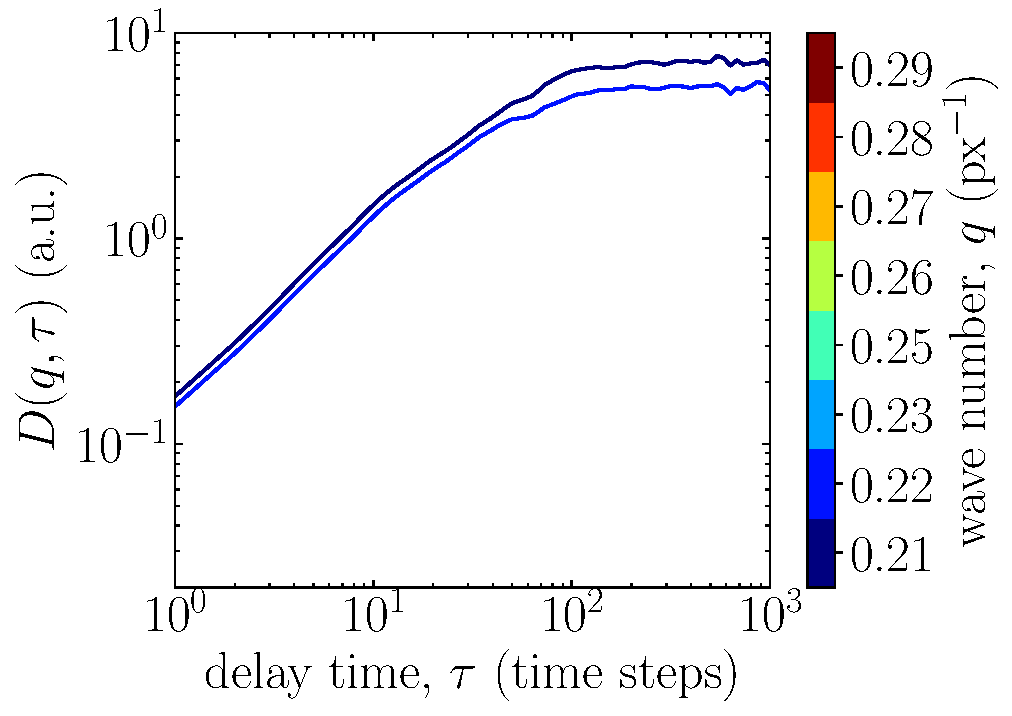
\includegraphics[width=\textwidth]
	{Sources/X-DFA/img_struc_func_vs_tau_q_range_001simulations10.pdf}}

	\only<3>{
	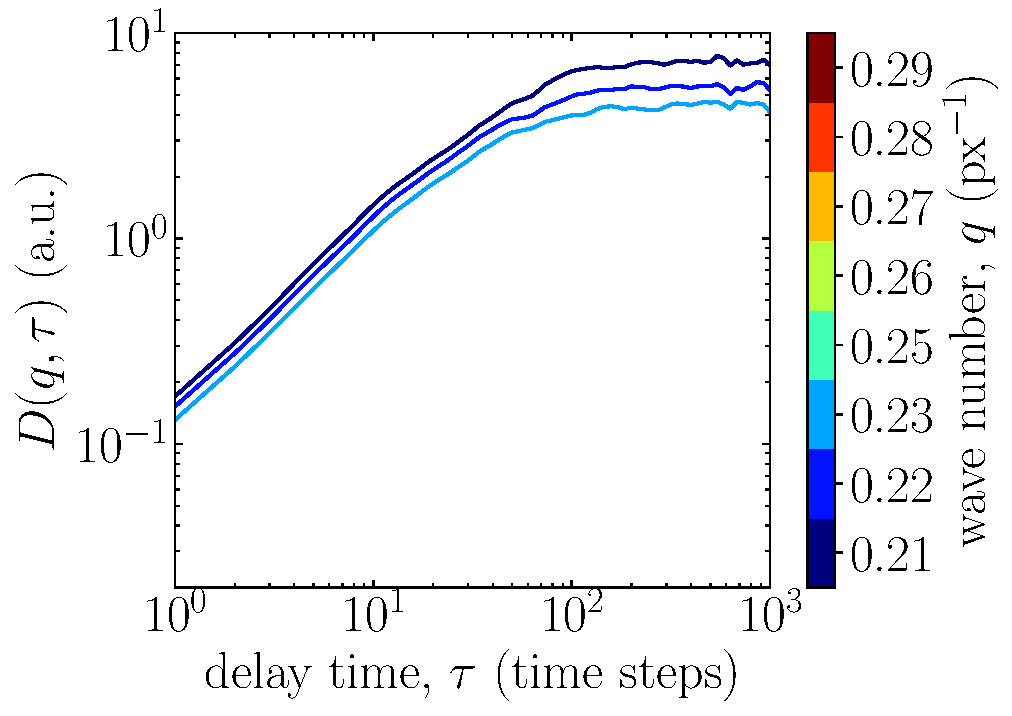
\includegraphics[width=\textwidth]
	{Sources/X-DFA/img_struc_func_vs_tau_q_range_002simulations10.pdf}}

	\visible<4->{
	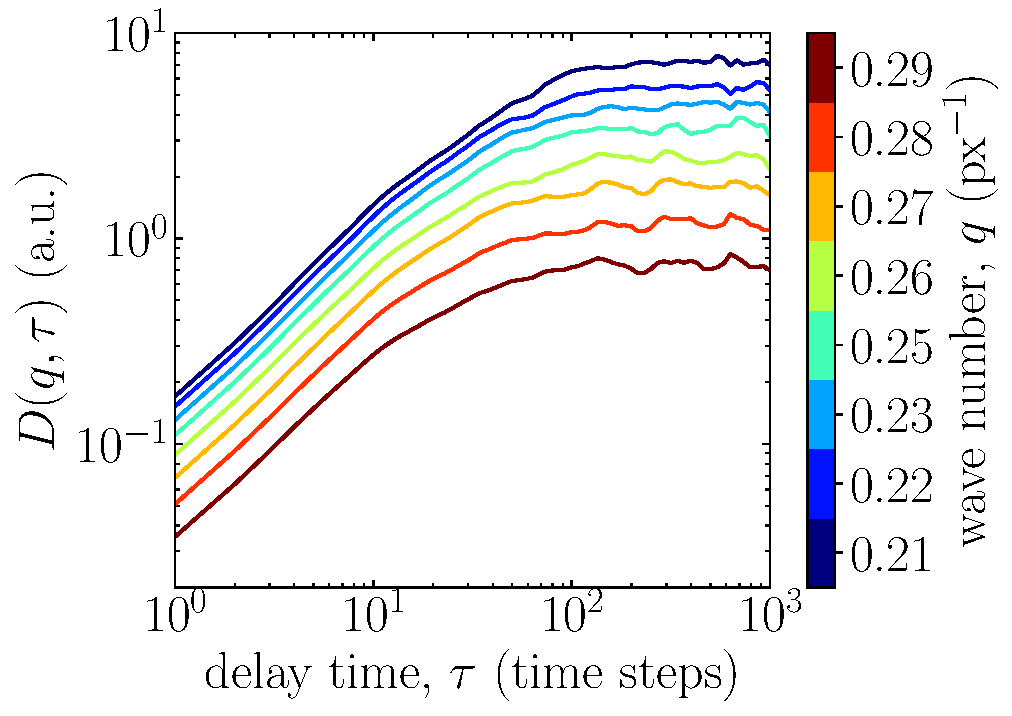
\includegraphics[width=\textwidth]
	{Sources/X-DFA/img_struc_func_vs_tau_q_range_007simulations10.pdf}}
	\end{textblock}


	\begin{textblock}{0.5}(0.02,0.63)
	\only<4>{\small
	\begin{align}
	D(q,\tau)
	&= \Big\langle |I(q, t+\tau) - I(q,t)|^2  \Big\rangle_t \nonumber \\
	&= A(q) 
	\left[1-\frac{\big\langle I^*(q,t) I(q,t+\tau) \big\rangle_t}
	{\big\langle |I(q,t)|^2 \big\rangle_t}\right] 
	+ B(q)\nonumber
	\end{align}
	}
	\visible<5->{\small
	\begin{align}
	D(q,\tau)
	&= \Big\langle |I(q, t+\tau) - I(q,t)|^2  \Big\rangle_t \nonumber \\
	&= A(q) 
	\bigg[1-
	\textcolor{red}{\underbrace{
			\frac{\big\langle I^*(q,t) I(q,t+\tau) \big\rangle_t}
			{\big\langle |I(q,t)|^2 \big\rangle_t}
	}}
	\bigg] 
	+ B(q)\nonumber
	\end{align}
	}
	\end{textblock}

	\begin{textblock}{0.3}(0.2,0.92)
	\visible<5->{
		\textcolor{red}{Image correlation function}
	}
	\end{textblock}

%	\begin{textblock}{0.5}(0.52,0.68)
%	\visible<6>{
%	\centering
%	\colorbox{lightblue}{
%	Linear space invariant imaging}
%	\small
%	\begin{align}
%	f(q,\tau) = \frac
%	{\langle \rho^*(q,t) \rho(q,t+\tau) \rangle_t}
%	{\langle |\rho(\mathbf{q},t)|^2 \rangle_t}
%	\nonumber
%	\end{align}
%
%	\normalsize
%	Intermediate scattering function
%	}
%	\end{textblock}
\end{frame}




\begin{frame}[noframenumbering]
\begin{textblock}{0.38}(0.02,0.02)
	\only<1>{
	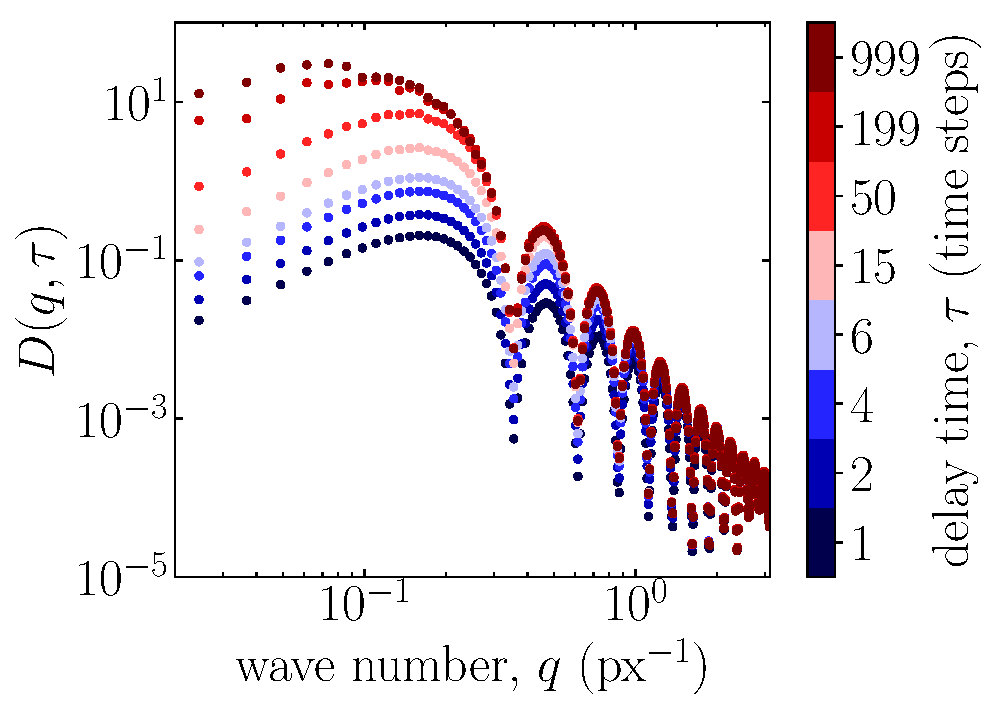
\includegraphics[width=\textwidth]
	{Sources/X-DFA/img_struc_func_vs_q_Ntau999_nPart10.pdf}}

	\visible<2->{
	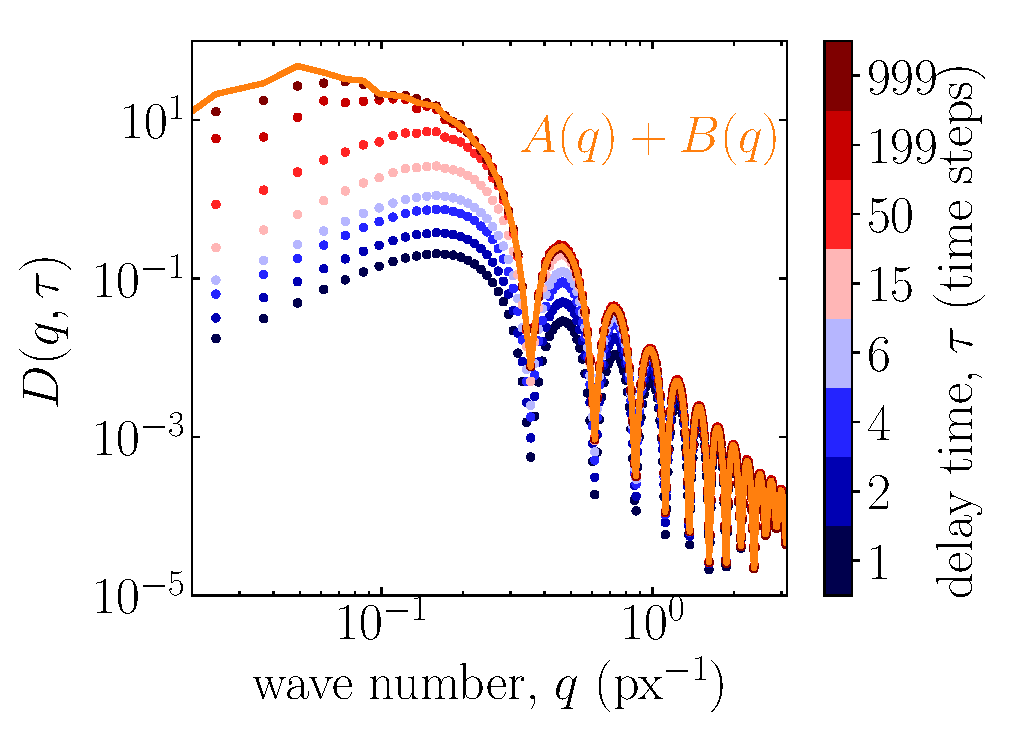
\includegraphics[width=\textwidth]
	{Sources/X-DFA/img_struc_func_vs_q_multiple_tau_simulations_nPart10with_A.eps}}
\end{textblock}

\begin{textblock}{0.38}(0.55,0.02)
	\visible<1->{
		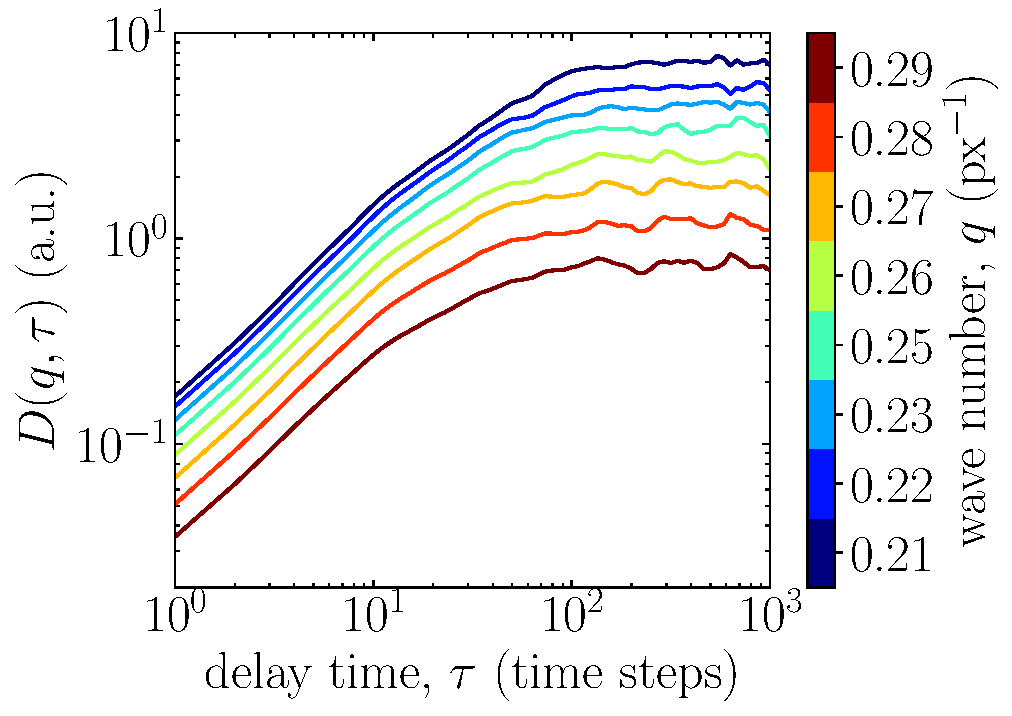
\includegraphics[width=\textwidth]
		{Sources/X-DFA/img_struc_func_vs_tau_q_range_007simulations10.pdf}}
\end{textblock}



\begin{textblock}{0.5}(0.02,0.5)
	\only<1>{
	\begin{align}
	D(q,\tau)
	&= \Big\langle |I(q, t+\tau) - I(q,t)|^2  \Big\rangle_t \nonumber \\
	&= A(q) 
	\bigg[1-
	\textcolor{red}{\underbrace{
			\frac{\big\langle I^*(q,t) I(q,t+\tau) \big\rangle_t}
			{\big\langle |I(q,t)|^2 \big\rangle_t}
	}}
	\bigg] 
	+ B(q)\nonumber
	\end{align}
	}
\end{textblock}

\begin{textblock}{0.3}(0.2,0.8)
	\only<1>{
		\textcolor{red}{Image correlation function}
	}
\end{textblock}

\begin{textblock}{0.5}(0.02,0.5)
	\visible<2->{
		\begin{align}
		D(q,\tau)
		&= \Big\langle |I(q, t+\tau) - I(q,t)|^2  \Big\rangle_t \nonumber \\
		&= \textcolor{orange}{A(q)}
		\bigg[1-
		\textcolor{red}{
				\frac{\big\langle I^*(q,t) I(q,t+\tau) \big\rangle_t}
				{\big\langle |I(q,t)|^2 \big\rangle_t}
		}
		\bigg] 
		+ \textcolor{darkgreen}{B(q)}\nonumber
		\end{align}
		
	\begin{itemize}
		\item $D(q, \tau \rightarrow 0) = \textcolor{darkgreen}{B(q)} = 0$
		\item $D(q, \tau \rightarrow \infty) = \textcolor{orange}{A(q) + B(q)}$
	\end{itemize}
	}
\end{textblock}

\begin{textblock}{0.5}(0.52,0.55)
	\only<1,2>{
	\centering
	\colorbox{lightblue}{
		Linear space invariant imaging}
	\begin{align}
	f(q,\tau) = \frac
	{\langle \rho^*(q,t) \rho(q,t+\tau) \rangle_t}
	{\langle |\rho(\mathbf{q},t)|^2 \rangle_t}
	\nonumber
	\end{align}
	
	Intermediate scattering function}
\end{textblock}


\begin{textblock}{0.38}(0.55,0.5)
	\visible<3->{
		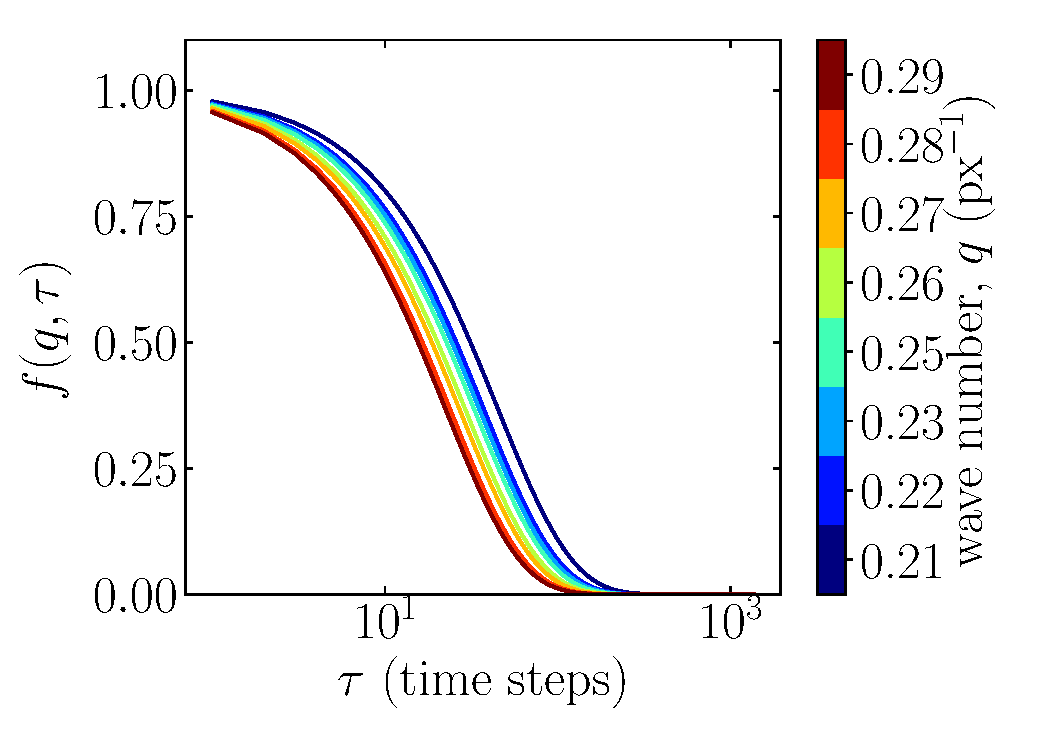
\includegraphics[width=\textwidth]
		{Sources/X-DFA/ISF_vs_tau.eps}}
\end{textblock}
\end{frame}

\frame{
\begin{tikzpicture}[remember picture,overlay]
\fill[blue1]
(current page.north west) rectangle ([xshift=0.55\paperwidth,yshift=0.33\paperheight]current page.west|-{pic cs:end});
\end{tikzpicture}

\begin{textblock}{0.62}(0.02,0.03)
	\textcolor{white}{
		\Large Intermediate scattering function $f(q,\tau)$}
\end{textblock}

\begin{textblock}{0.35}(0.02,0.1)
	\visible<1->{
		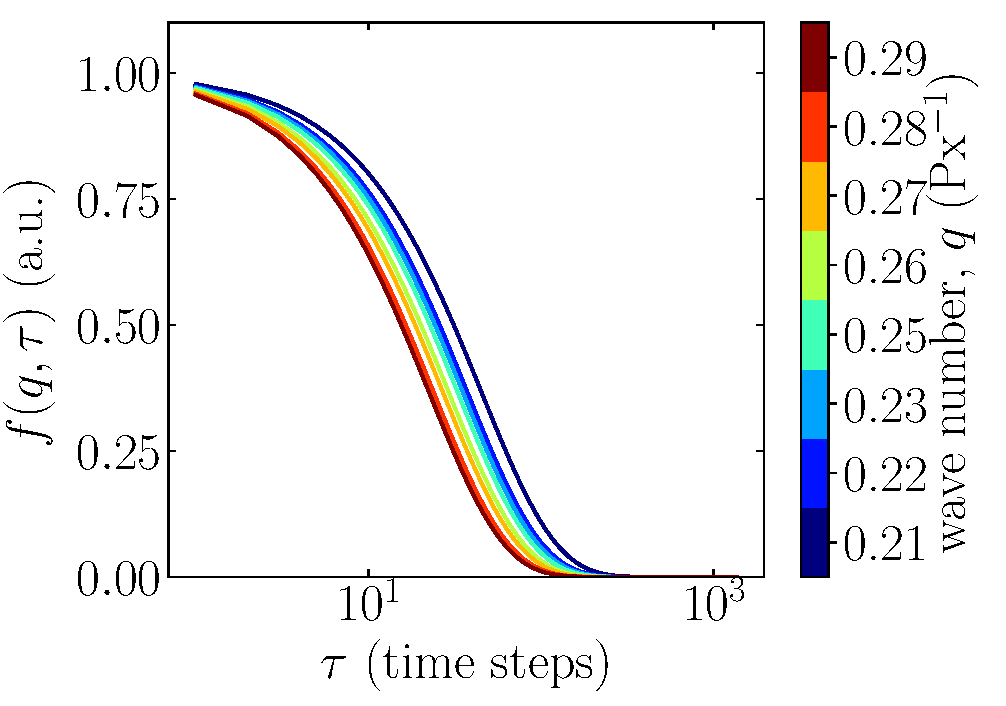
\includegraphics[width=\textwidth]
		{Sources/X-DFA/ISF_vs_tau.pdf}}
\end{textblock}



\begin{textblock}{0.35}(0.02,0.55)
	\visible<2->{
		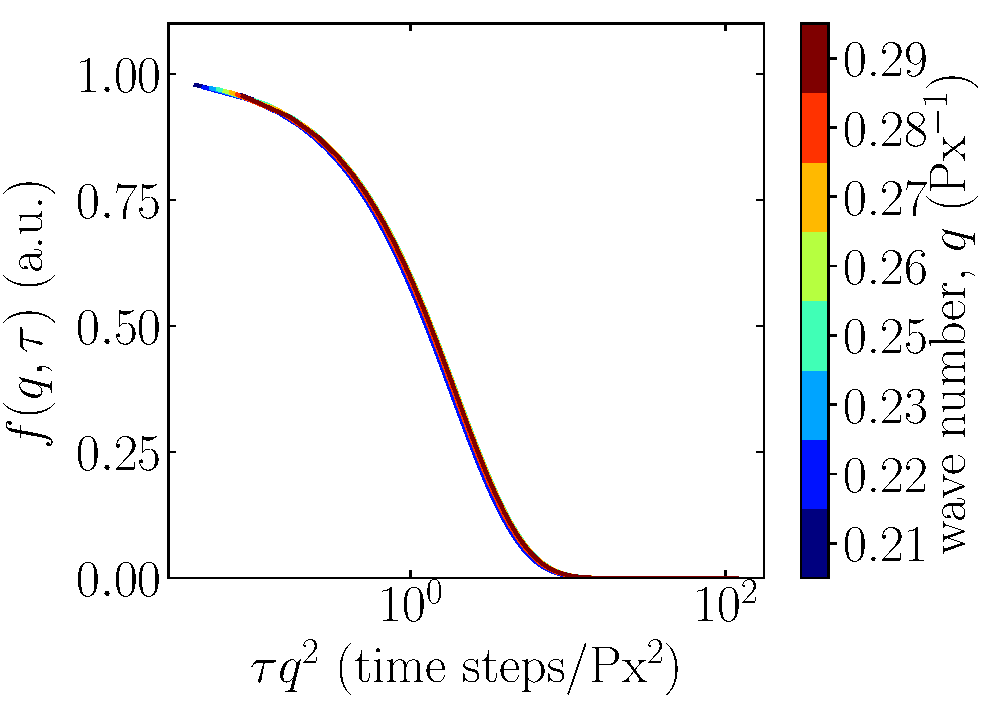
\includegraphics[width=\textwidth]
		{Sources/X-DFA/ISF_vs_tau_q_squared.pdf}}
\end{textblock}

\begin{textblock}{0.5}(0.4,0.15)
	\centering
	\visible<1->{
		Brownian motion:\\
		$f(q,\tau) = \exp(- q^2 \tau/\tau_\text{D})$
	}
\end{textblock}

\begin{textblock}{0.5}(0.4,0.33)
	\visible<2->{
		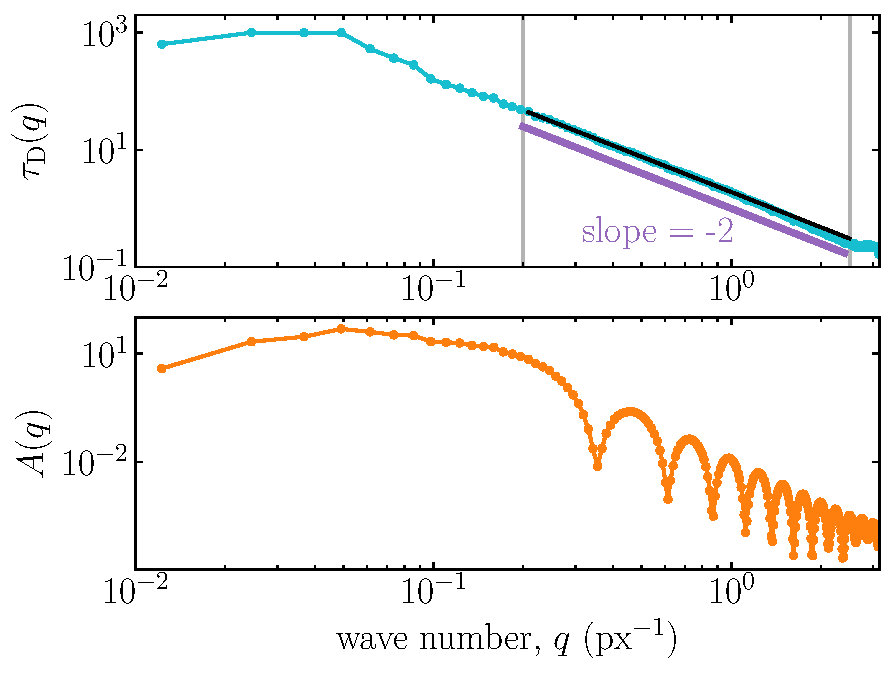
\includegraphics[width=\textwidth]
		{Sources/X-DFA/FitParameters.pdf}}
\end{textblock}

\begin{textblock}{0.5}(0.4,0.33)
	\visible<2->{\textcolor{red}{take out A(q)}}
\end{textblock}
}




\frame{
\begin{tikzpicture}[remember picture,overlay]
\fill[blue1]
(current page.north west) rectangle ([xshift=0.75\paperwidth,yshift=0.33\paperheight]current page.west|-{pic cs:end});
\end{tikzpicture}

\begin{textblock}{0.9}(0.02,0.03)
	\textcolor{white}{
		\Large Accuracy of X-DFA: Varying the number of particles}
\end{textblock}

\begin{textblock}{0.28}(0.03,0.12)
\centering
10 particles\\[0.1cm]

\fbox{\parbox{\textwidth}{
\movie[width = \textwidth]
{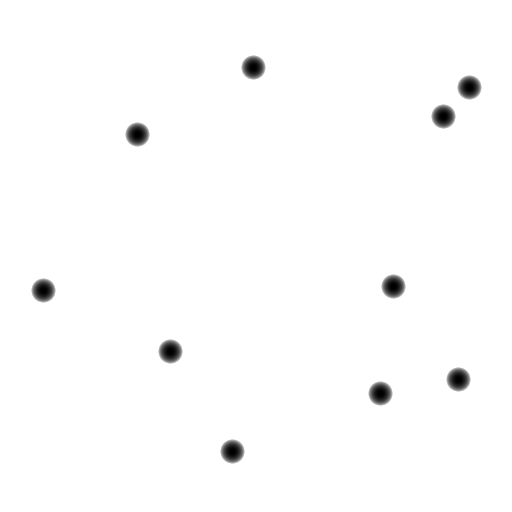
\includegraphics[width=\textwidth]{Sources/X-DFA/10_particles_fake_img.png}}
{Sources/X-DFA/10_part_1900-2100.avi}}}
\\
\vspace{1cm}
\colorbox{lightblue}{
6\%}
\end{textblock}

\begin{textblock}{0.28}(0.345,0.12)
\centering
1000 particles\\[0.1cm]

\fbox{\parbox{\textwidth}{
\movie[width = \textwidth]
{
\includegraphics[width=\textwidth]{Sources/X-DFA/1000_particles_fake_img.png}}
{Sources/X-DFA/1000_particles.avi}}}
\\
\vspace{1cm}
\colorbox{lightblue}{
2\%}
\end{textblock}

\begin{textblock}{0.28}(0.66,0.12)
\centering
$100\,000$ particles\\[0.1cm]

\fbox{\parbox{\textwidth}{
\movie[width = \textwidth]
{
\includegraphics[width=\textwidth]{Sources/X-DFA/100000_particles_fake_img.png}}
{Sources/X-DFA/100000_particles.avi}}}
\\
\vspace{1cm}
\colorbox{lightblue}{
2\%}\\[0.1cm]

\colorbox{red}{PIV off by $\approx 650\%$}
\end{textblock}

\begin{textblock}{0.9}(0.05,0.74)
	\centering
	Deviation from the simulation input:
\end{textblock}
}






